%% Generado por html2tex.py desde temas.json (fis). No editar a mano: corregir la clase en el .js del sitio y regenerar.
\parteciencia{fis}
\chapter{Ondas}
%% =====================================================================
%% fis_ondas_elementos
\section[Elementos de las ondas]{Elementos de las ondas}
\modcomun\ \ {\color{gris}\itshape Qué es una onda, ondas mecánicas y electromagnéticas, amplitud, longitud de onda, período y frecuencia, la relación v = \ensuremath{\lambda}f, qué cambia y qué no al pasar de un medio a otro, y la propagación de la luz en línea recta.\par}
\subsection{Qué es una onda}
Una \textbf{onda} es una perturbación que se propaga y \textbf{transporta energía de un lugar a otro sin transportar materia}. Cuando pasa una ola, un corcho en el agua sube y baja, pero no viaja con la ola.

 

Según lo que necesitan para propagarse, las ondas son de dos tipos:

 
\begin{itemize}
  \item \textbf{Mecánicas:} necesitan un \textbf{medio material} (sólido, líquido o gas) que vibre. Ejemplos: el sonido, las olas del mar, una onda en una cuerda, las ondas sísmicas. No se propagan en el vacío.
  \item \textbf{Electromagnéticas:} son oscilaciones de campos eléctricos y magnéticos y \textbf{no necesitan medio}: se propagan también en el vacío. Ejemplos: la luz, las ondas de radio, las microondas, los rayos X.
\end{itemize}
 

Según cómo vibra el medio respecto de la dirección de avance, las ondas son \textbf{transversales} (vibran de forma perpendicular al avance, como una cuerda o la luz) o \textbf{longitudinales} (vibran en la misma dirección del avance, como el sonido).

  
\begin{clave}[{Recuerda}] La luz del Sol llega a la Tierra atravesando el espacio vacío; el sonido de una explosión en el Sol, no. Por eso en el espacio no se escucha nada, pero sí se ve.\end{clave}
 
\begin{clave}[{En la PAES}] La prueba de Física pregunta sobre todo por ondas electromagnéticas: luz, radio, microondas, infrarrojo, rayos X. Las ideas de este tema (amplitud, frecuencia, longitud de onda, rapidez) valen para todas las ondas.\end{clave}
\subsection{Elementos de una onda}
\begin{itemize}
  \item \textbf{Cresta y valle:} los puntos más alto y más bajo de la onda.
  \item \textbf{Amplitud ($A$):} distancia desde la posición de equilibrio hasta una cresta (o un valle). Se relaciona con la \textbf{energía} o intensidad de la onda. No es la distancia de cresta a valle: esa vale $2A$.
  \item \textbf{Longitud de onda ($\lambda$):} distancia entre dos crestas (o dos valles) consecutivas. Es la longitud de un ciclo completo. Se mide en metros.
  \item \textbf{Período ($T$):} tiempo que tarda en completarse un ciclo. Se mide en segundos.
  \item \textbf{Frecuencia ($f$):} número de ciclos por segundo. Se mide en hertz (Hz = 1/s).
\end{itemize}
 \[ f = \dfrac{1}{T} \qquad\qquad T = \dfrac{1}{f} \] 

Si una fuente vibra 50 veces en 2 s, su frecuencia es $f = 50/2 = 25$ Hz y su período es $T = 1/25 = 0{,}04$ s.

  
\begin{center}
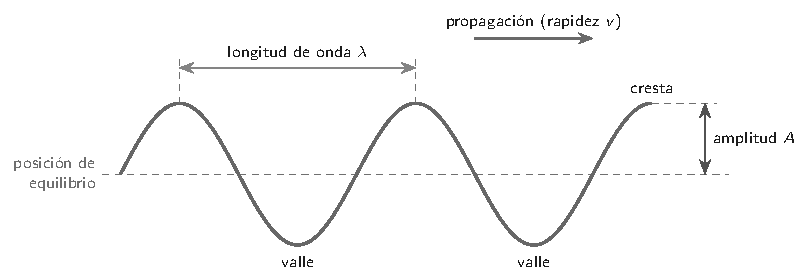
\includegraphics[max width=0.92\linewidth,max height=8.5cm]{fis/ond_elementos}
\end{center}
 
\begin{clave}[{Recuerda}] Prefijos frecuentes: kHz $= 10^3$ Hz, MHz $= 10^6$ Hz, GHz $= 10^9$ Hz; nm $= 10^{-9}$ m, $\mu$m $= 10^{-6}$ m.\end{clave}
\subsection{Rapidez de propagación: v = \ensuremath{\lambda}f}
En un período $T$ la onda avanza exactamente una longitud de onda $\lambda$. Por eso su rapidez de propagación es:

 \[ v = \dfrac{\lambda}{T} = \lambda\, f \] 

De aquí salen las otras dos formas: $\lambda = \dfrac{v}{f}$ y $f = \dfrac{v}{\lambda}$.

 

Todas las ondas electromagnéticas viajan en el vacío con la misma rapidez, la \textbf{rapidez de la luz}:

 \[ c = 3{,}0\times10^{8}\ \text{m/s} = 300\,000\ \text{km/s} \] 

\textbf{Ejemplo.} Una radio FM transmite a $f = 100$ MHz $= 1{,}0\times10^{8}$ Hz. Su longitud de onda es $\lambda = \dfrac{3{,}0\times10^{8}}{1{,}0\times10^{8}} = 3{,}0$ m.

  
\begin{clave}[{Qué depende de qué}] · La \textbf{rapidez} la fija el \textbf{medio}: en un mismo medio, todas las ondas del mismo tipo viajan igual de rápido.\par · La \textbf{frecuencia} la fija la \textbf{fuente} que produce la onda.\par · La \textbf{longitud de onda} se ajusta: $\lambda = v/f$.\end{clave}
 
\begin{clave}[{Recuerda}] En un mismo medio, si la frecuencia se duplica, la longitud de onda se reduce a la mitad: $\lambda$ y $f$ son \textbf{inversamente proporcionales} y su producto, la rapidez, no cambia.\end{clave}
 
\begin{center}\small
\begin{tabular}{@{}ll@{}}
\toprule
\textbf{Onda y medio} & \textbf{Rapidez aproximada} \\
\midrule
Luz en el vacío (y en el aire) & $3{,}0\times10^{8}$ m/s \\
Luz en el agua & $2{,}25\times10^{8}$ m/s \\
Luz en el vidrio & $2{,}0\times10^{8}$ m/s \\
Sonido en el aire & 340 m/s \\
\bottomrule
\end{tabular}
\end{center}
\subsection{Cuando la onda cambia de medio}
Cuando una onda pasa de un medio a otro (por ejemplo, la luz del aire al vidrio):

 
\begin{itemize}
  \item La \textbf{frecuencia no cambia}: la impone la fuente, y cada cresta que llega a la frontera genera una cresta al otro lado.
  \item La \textbf{rapidez cambia}, porque depende del medio.
  \item La \textbf{longitud de onda cambia} en la misma proporción que la rapidez: $\lambda = v/f$.
\end{itemize}
 

\textbf{Ejemplo.} Luz de $f = 6{,}0\times10^{14}$ Hz tiene en el vacío $\lambda = 5{,}0\times10^{-7}$ m. Entra a un material donde su rapidez es la mitad, $1{,}5\times10^{8}$ m/s. Allí la frecuencia sigue siendo $6{,}0\times10^{14}$ Hz y la longitud de onda es

 \[ \lambda = \dfrac{1{,}5\times10^{8}}{6{,}0\times10^{14}} = 2{,}5\times10^{-7}\ \text{m} \] 

La rapidez bajó a la mitad y la longitud de onda también.

  
\begin{clave}[{Recuerda}] El color de la luz está ligado a su frecuencia. Como la frecuencia no cambia al pasar al agua o al vidrio, una luz roja sigue siendo roja dentro del agua.\end{clave}
 
\begin{clave}[{Cómo razonar}] Si te dicen que la onda «entra a otro medio», marca la frecuencia como constante y calcula lo demás con $v = \lambda f$. Si te dicen que la fuente cambia su frecuencia «en el mismo medio», marca la rapidez como constante.\end{clave}
\subsection{La luz viaja en línea recta}
En un medio homogéneo (aire, agua, vidrio) la luz se propaga en \textbf{línea recta}. Para representarla usamos \textbf{rayos}: líneas con una flecha que indica hacia dónde viaja la luz.

 
\begin{itemize}
  \item \textbf{Sombras.} Un objeto opaco bloquea los rayos y detrás queda una zona sin luz con la forma del objeto. Con una fuente pequeña la sombra es nítida; con una fuente grande aparece además una \textbf{penumbra}.
  \item \textbf{Eclipses.} Un eclipse de Sol es la sombra de la Luna sobre la Tierra; uno de Luna, la sombra de la Tierra sobre la Luna.
  \item \textbf{Cámara oscura.} Una caja con un orificio pequeño forma en la cara opuesta una \textbf{imagen invertida} de lo que está afuera: los rayos de la parte alta del objeto cruzan el orificio y llegan abajo, y los de la parte baja llegan arriba.
\end{itemize}
  
\begin{clave}[{Sombras y proporciones}] Con una fuente puntual, la sombra es una ampliación del objeto. Si un objeto de 10 cm está a 1 m de la ampolleta y la pared está a 3 m de la ampolleta, la sombra mide $10 \cdot \dfrac{3}{1} = 30$ cm.\end{clave}
 
\begin{clave}[{Recuerda}] La luz sí puede doblar sus rayos: al cambiar de medio (refracción) o al rebotar (reflexión). Lo que no hace es curvarse dentro de un mismo medio homogéneo.\end{clave}
\subsection{Lo clave del tema}
\begin{center}\small
\begin{tabularx}{\linewidth}{@{}>{\raggedright\arraybackslash\hsize=0.79\hsize}X>{\raggedright\arraybackslash\hsize=1.36\hsize}X>{\raggedright\arraybackslash\hsize=0.34\hsize}X>{\raggedright\arraybackslash\hsize=1.51\hsize}X@{}}
\toprule
\textbf{Concepto} & \textbf{Qué es} & \textbf{Unidad} & \textbf{Qué lo determina} \\
\midrule
Amplitud $A$ & desde el equilibrio hasta una cresta & m & la energía que entrega la fuente \\
Longitud de onda $\lambda$ & distancia entre crestas consecutivas & m & $\lambda = v/f$ \\
Período $T$ & tiempo de un ciclo & s & la fuente; $T = 1/f$ \\
Frecuencia $f$ & ciclos por segundo & Hz & la fuente; no cambia al cambiar de medio \\
Rapidez $v$ & qué tan rápido avanza la onda & m/s & el medio; $v = \lambda f$ \\
\bottomrule
\end{tabularx}
\end{center}
 
\begin{clave}[{Recuerda}] · Mecánicas: necesitan medio (sonido). Electromagnéticas: viajan también en el vacío, a $c = 3{,}0\times10^{8}$ m/s.\par · En un mismo medio, más frecuencia significa menor longitud de onda.\par · Al cambiar de medio cambian $v$ y $\lambda$; la frecuencia se mantiene.\par · La luz viaja en línea recta: sombras, eclipses y cámara oscura.\end{clave}
 
\begin{clave}[{Método PAES}] 1. Anota los datos con sus unidades y pásalos a SI (MHz a Hz, nm a m). 2. Decide qué se mantiene: la rapidez (mismo medio) o la frecuencia (cambio de medio). 3. Usa $v = \lambda f$ despejando lo que te piden. 4. Revisa el orden de magnitud: la luz visible tiene $\lambda$ de cientos de nanómetros y $f$ cercana a $10^{14}$--$10^{15}$ Hz.\end{clave}
\begin{elejemplo}{PAES Invierno 2027, adaptada}
Una emisora de radio emite ondas electromagnéticas de frecuencia $6{,}0\times10^{7}$ Hz, que se propagan en el aire con una rapidez de $3{,}0\times10^{8}$ m/s.

¿Cuál es la longitud de onda de estas ondas en el aire?
\alts{0,2 m}{5,0 m}{$5{,}0\times10^{3}$ m}{$1{,}8\times10^{16}$ m}
\solucion{\textbf{Paso 1. ¿Qué nos piden?} La longitud de onda, conociendo la frecuencia y la rapidez de la onda.

\textbf{Paso 2. Elige la relación.} De $v = \lambda f$ se despeja $\lambda = \dfrac{v}{f}$.

\textbf{Paso 3. Calcula.} $\lambda = \dfrac{3{,}0\times10^{8}}{6{,}0\times10^{7}} = 0{,}5\times10^{1} = 5{,}0$ m.

\textbf{Respuesta:} 5,0 m.

\textbf{¿Por qué no las otras?} 0,2 m sale de invertir la división ($f/v$). $5{,}0\times10^{3}$ m resulta de restar mal los exponentes. $1{,}8\times10^{16}$ m es el producto $v \cdot f$, que no tiene unidades de longitud.

\textbf{\color{cienciaD}Para recordar.} Longitud de onda = rapidez dividida por frecuencia.}{B}
\end{elejemplo}

%% =====================================================================
%% fis_espectro
\section[Espectro electromagnético]{Espectro electromagnético}
\modcomun\ \ {\color{gris}\itshape El orden de las ondas electromagnéticas según su longitud de onda y su frecuencia, los usos tecnológicos de cada rango, la luz visible, la rapidez común en el vacío, y la interferencia y la difracción en términos cualitativos.\par}
\subsection{El espectro electromagnético}
Las ondas electromagnéticas forman una familia continua llamada \textbf{espectro electromagnético}. Todas son la misma clase de onda; lo que cambia es su \textbf{frecuencia} y, por lo tanto, su \textbf{longitud de onda}.

 

Ordenadas de \textbf{menor a mayor frecuencia} (y de mayor a menor longitud de onda):

 
\begin{center}
\textbf{radio \ensuremath{\rightarrow} microondas \ensuremath{\rightarrow} infrarrojo \ensuremath{\rightarrow} luz visible \ensuremath{\rightarrow} ultravioleta \ensuremath{\rightarrow} rayos X \ensuremath{\rightarrow} rayos gamma}
\end{center}
 
\begin{itemize}
  \item Todas viajan en el vacío a la misma rapidez, $c = 3{,}0\times10^{8}$ m/s.
  \item Como $c = \lambda f$, si la frecuencia aumenta, la longitud de onda disminuye.
  \item La \textbf{energía} que transporta la radiación aumenta con la frecuencia. Por eso el ultravioleta, los rayos X y los rayos gamma pueden dañar las células.
\end{itemize}
  
\begin{center}
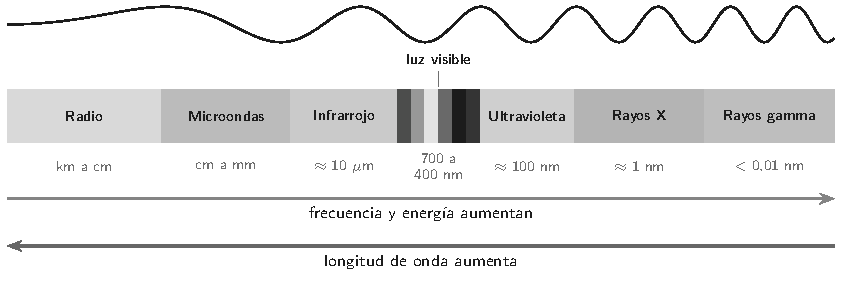
\includegraphics[max width=0.92\linewidth,max height=8.5cm]{fis/ond_espectro}
\end{center}
 
\gatotip[\gatogris]{\textbf{Truco para recordar el orden.} Piensa en el daño: radio y microondas atraviesan tu cuerpo sin dañarlo; el ultravioleta quema la piel; los rayos X y gamma son peligrosos. El daño crece con la frecuencia.}
\subsection{Usos tecnológicos de cada rango}
\begin{center}\small
\begin{tabularx}{\linewidth}{@{}>{\raggedright\arraybackslash\hsize=0.58\hsize}X>{\raggedright\arraybackslash\hsize=0.88\hsize}X>{\raggedright\arraybackslash\hsize=1.54\hsize}X@{}}
\toprule
\textbf{Rango} & \textbf{Longitud de onda típica} & \textbf{Usos y ejemplos} \\
\midrule
Ondas de radio & km a cm & radio AM y FM, televisión abierta, radiotelescopios, comunicación con barcos y aviones \\
Microondas & cm a mm & hornos microondas, wifi, bluetooth, telefonía móvil, radar, comunicación satelital, GPS \\
Infrarrojo & µm & controles remotos, cámaras térmicas y de visión nocturna, calefactores, fibra óptica; todo cuerpo tibio emite infrarrojo \\
Luz visible & 700 a 400 nm & visión, iluminación, fotografía, láser, pantallas \\
Ultravioleta & \textasciitilde{}100 nm & esterilización de agua e instrumentos, detección de billetes falsos, síntesis de vitamina D; produce quemaduras solares \\
Rayos X & \textasciitilde{}1 nm & radiografías, escáneres de equipaje, estudio de cristales \\
Rayos gamma & < 0,01 nm & radioterapia contra el cáncer, esterilización de alimentos y material médico \\
\bottomrule
\end{tabularx}
\end{center}
 
\begin{clave}[{Recuerda}] Los celulares, el wifi y el horno usan microondas, pero de distinta potencia: el horno concentra mucha energía en un espacio cerrado; el teléfono emite muy poca. La radiación de radio y microondas es \textbf{no ionizante}; la de rayos X y gamma es \textbf{ionizante}.\end{clave}
\subsection{La luz visible y los colores}
La \textbf{luz visible} es la pequeña parte del espectro que detectan nuestros ojos, entre unos \textbf{700 nm} (rojo) y \textbf{400 nm} (violeta).

 
\begin{center}\small
\begin{tabular}{@{}ll@{}}
\toprule
\textbf{Color} & \textbf{Longitud de onda aproximada} \\
\midrule
Rojo & 700 a 620 nm \\
Naranjo & 620 a 590 nm \\
Amarillo & 590 a 570 nm \\
Verde & 570 a 495 nm \\
Azul & 495 a 450 nm \\
Violeta & 450 a 400 nm \\
\bottomrule
\end{tabular}
\end{center}
  
\begin{itemize}
  \item El \textbf{rojo} tiene la mayor longitud de onda y la menor frecuencia de la luz visible.
  \item El \textbf{violeta} tiene la menor longitud de onda y la mayor frecuencia.
  \item Más allá del rojo está el \textbf{infrarrojo} («bajo el rojo»); más allá del violeta, el \textbf{ultravioleta}.
  \item La luz blanca del Sol es una mezcla de todos los colores.
\end{itemize}
 
\begin{clave}[{Recuerda}] En el vacío la luz roja y la violeta viajan igual de rápido. Lo que las distingue es su frecuencia (y su longitud de onda), no su rapidez.\end{clave}
\subsection{Interferencia y difracción}
\textbf{Interferencia.} Cuando dos ondas coinciden en un mismo lugar, se superponen. Si llegan cresta con cresta se refuerzan (\textbf{interferencia constructiva}); si llega cresta con valle se anulan (\textbf{interferencia destructiva}).

 

En el \textbf{experimento de la doble rendija de Young}, luz de una sola fuente pasa por dos rendijas muy finas y muy juntas. En la pantalla aparecen \textbf{franjas} claras (interferencia constructiva) y oscuras (destructiva). Para que se vea el patrón, las rendijas deben ser de un tamaño comparable a la longitud de onda y la luz debe ser de una sola frecuencia, como la de un láser.

 

\textbf{Difracción.} Es la capacidad de una onda de \textbf{rodear obstáculos y abrirse al pasar por una abertura}. Se nota cuando la abertura o el obstáculo tiene un tamaño parecido a la longitud de onda.

  
\begin{ejemplo}[{Ejemplos}] · Las ondas de radio AM, con longitudes de onda de cientos de metros, rodean cerros y edificios: se reciben aunque no se vea la antena.\par · La luz, con longitudes de onda de cientos de nanómetros, no rodea una pared, pero sí se difracta en una rendija del grosor de un cabello.\par · Los colores de un CD o de una pompa de jabón se deben a la interferencia de la luz.\end{ejemplo}
 
\begin{clave}[{Recuerda}] La interferencia y la difracción son comportamientos propios de las ondas. El experimento de Young fue una prueba clave de que la luz es una onda.\end{clave}
\subsection{Lo clave del tema}
\begin{center}\small
\begin{tabularx}{\linewidth}{@{}>{\raggedright\arraybackslash\hsize=0.62\hsize}X>{\raggedright\arraybackslash\hsize=1.38\hsize}X@{}}
\toprule
\textbf{Idea} & \textbf{Lo que debes saber} \\
\midrule
Orden del espectro & radio, microondas, infrarrojo, visible, ultravioleta, rayos X, gamma: la frecuencia y la energía aumentan, la longitud de onda disminuye \\
Rapidez & todas viajan a $3{,}0\times10^{8}$ m/s en el vacío \\
Luz visible & entre el infrarrojo y el ultravioleta; rojo (700 nm, menor $f$) a violeta (400 nm, mayor $f$) \\
Interferencia & superposición de ondas: franjas claras y oscuras (Young) \\
Difracción & la onda rodea obstáculos o se abre en aberturas de tamaño comparable a $\lambda$ \\
\bottomrule
\end{tabularx}
\end{center}
 
\begin{clave}[{Método PAES}] 1. Ubica cada radiación en el espectro antes de comparar. 2. Recuerda que la rapidez en el vacío es la misma para todas. 3. En difracción, compara el tamaño de la abertura con la longitud de onda.\end{clave}
\begin{elejemplo}{Estilo PAES}
¿Cuál de las siguientes opciones ordena estas radiaciones de \textbf{menor a mayor frecuencia}: rayos X, ondas de radio, luz visible y microondas?
\begin{center}
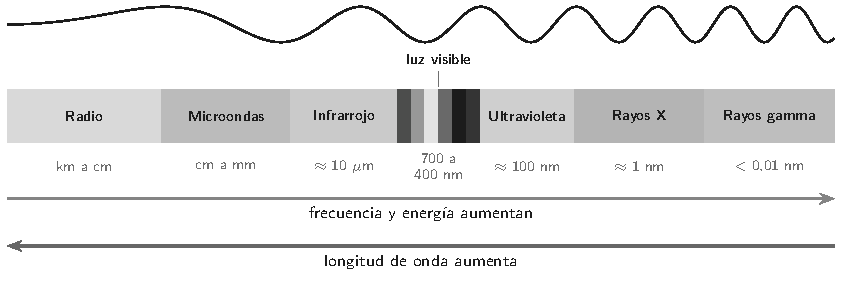
\includegraphics[max width=0.92\linewidth,max height=8.5cm]{fis/ond_espectro}
\end{center}
\altslargas{rayos X, luz visible, microondas, ondas de radio}{ondas de radio, microondas, luz visible, rayos X}{microondas, ondas de radio, rayos X, luz visible}{luz visible, microondas, ondas de radio, rayos X}
\solucion{\textbf{Paso 1. ¿Qué nos piden?} Ordenar cuatro radiaciones según su frecuencia, de menor a mayor.

\textbf{Paso 2. Ubícalas en el espectro.} De izquierda a derecha (frecuencia creciente): radio, microondas, infrarrojo, visible, ultravioleta, rayos X, gamma.

\textbf{Paso 3. Extrae las cuatro.} Ondas de radio, microondas, luz visible, rayos X.

\textbf{Respuesta:} ondas de radio, microondas, luz visible, rayos X.

\textbf{¿Por qué no las otras?} «Rayos X, luz visible, microondas, ondas de radio» es el orden inverso, de mayor a menor frecuencia (que coincide con el orden de menor a mayor longitud de onda). Las otras dos mezclan el orden: las microondas tienen mayor frecuencia que las ondas de radio, y la luz visible menor que los rayos X.

\textbf{\color{cienciaD}Para recordar.} Radio, microondas, infrarrojo, visible, ultravioleta, X, gamma: la frecuencia sube.}{B}
\end{elejemplo}

%% =====================================================================
%% fis_luz
\section[Reflexión, refracción y color]{Reflexión, refracción y color}
\modcomun\ \ {\color{gris}\itshape Qué le ocurre a la luz al llegar a un material (absorción, reflexión y transmisión), la ley de reflexión, la refracción como cambio de rapidez y de dirección y la formación de los colores de los objetos.\par}
\subsection{Qué le pasa a la luz al llegar a un material}
Cuando la luz llega a la superficie de un material, se reparte de tres formas:

 
\begin{itemize}
  \item \textbf{Reflexión:} una parte rebota y vuelve al medio del que venía.
  \item \textbf{Absorción:} una parte es absorbida por el material y su energía lo calienta.
  \item \textbf{Transmisión:} una parte atraviesa el material y sigue al otro lado.
\end{itemize}
 

La energía se conserva: \textbf{incidente = reflejada + absorbida + transmitida}. Si se mide que pasa el 70 \% de la radiación, el material transmite el 70 \%; el 30 \% restante se reflejó o se absorbió.

 

Según cuánto transmiten, los materiales son \textbf{transparentes} (dejan pasar la luz y se ve con nitidez a través de ellos: vidrio, agua), \textbf{translúcidos} (dejan pasar luz, pero no se ve con nitidez: papel mantequilla, vidrio esmerilado) u \textbf{opacos} (no dejan pasar luz: madera, metal).

  
\begin{clave}[{Recuerda}] Un material puede ser transparente a un rango del espectro y opaco a otro. El vidrio deja pasar la luz visible pero absorbe buena parte del ultravioleta; el cuerpo humano es opaco a la luz pero deja pasar los rayos X.\end{clave}
 
\begin{ejemplo}[{Ejemplo PAES}] Se recomienda usar protector solar aunque estés dentro del agua: el agua \textbf{transmite} parte de la radiación ultravioleta, que llega a tu piel.\end{ejemplo}
\subsection{Reflexión de la luz}
Para describir la reflexión se usa la \textbf{normal}: una recta perpendicular a la superficie en el punto donde llega el rayo. Los ángulos se miden \textbf{desde la normal}, no desde la superficie.

 

\textbf{Ley de reflexión:}

 
\begin{itemize}
  \item El ángulo de incidencia es igual al ángulo de reflexión: $\alpha = \beta$.
  \item El rayo incidente, el rayo reflejado y la normal están en un mismo plano.
\end{itemize}
 

\textbf{Reflexión especular y difusa.} En una superficie lisa (espejo, agua quieta) los rayos paralelos se reflejan paralelos y se forma una imagen. En una superficie rugosa (papel, pared) cada rayo se refleja en una dirección distinta: la luz se esparce y no se forma imagen, pero el objeto se ve desde todos lados.

 

En la reflexión no cambian ni la rapidez, ni la frecuencia, ni la longitud de onda: la luz sigue en el mismo medio.

  
\begin{center}
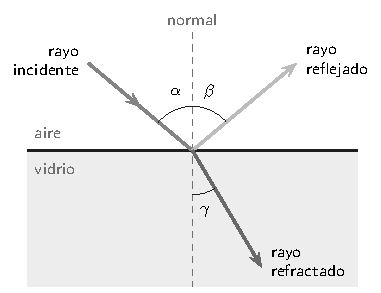
\includegraphics[max width=0.92\linewidth,max height=8.5cm]{fis/ond_reflex_refrac}
\end{center}
 
\begin{clave}[{Recuerda}] Si un rayo forma 30° con la superficie del espejo, forma 60° con la normal: el ángulo de incidencia es 60° y el de reflexión también.\end{clave}
\subsection{Refracción de la luz}
La \textbf{refracción} es el cambio de dirección que experimenta la luz al pasar de un medio a otro con incidencia oblicua. Su causa es el \textbf{cambio de rapidez}.

 

El \textbf{índice de refracción} $n$ indica cuánto se frena la luz en un medio: $n = c/v$. Mientras mayor es $n$, más lenta va la luz.

 
\begin{center}\small
\begin{tabular}{@{}ll@{}}
\toprule
\textbf{Medio} & \textbf{$n$ aproximado} \\
\midrule
Aire & 1,00 \\
Agua & 1,33 \\
Vidrio & 1,5 \\
Diamante & 2,4 \\
\bottomrule
\end{tabular}
\end{center}
 
\begin{itemize}
  \item Si la luz pasa a un medio \textbf{más lento} (mayor $n$), el rayo refractado \textbf{se acerca a la normal}: $\gamma < \alpha$.
  \item Si pasa a un medio \textbf{más rápido} (menor $n$), \textbf{se aleja de la normal}.
  \item Si incide \textbf{perpendicularmente}, no cambia de dirección, aunque sí de rapidez.
\end{itemize}
  
\begin{clave}[{Qué cambia y qué no}] Al refractarse, cambian la \textbf{rapidez}, la \textbf{longitud de onda} y la \textbf{dirección}. La \textbf{frecuencia} (y por lo tanto el color) \textbf{no cambia}.\end{clave}
 
\begin{ejemplo}[{Ejemplos}] · Una cuchara se ve quebrada en un vaso con agua.\par · El fondo de una piscina parece menos profundo de lo que es: la luz que sale del agua se aleja de la normal y el ojo la prolonga en línea recta desde un punto más alto.\end{ejemplo}
 
\begin{clave}[{Reflexión total interna}] Si la luz va de un medio más lento a uno más rápido (del vidrio al aire) con un ángulo mayor que un cierto \textbf{ángulo límite}, no sale: se refleja por completo. Es la base de la fibra óptica.\end{clave}
\subsection{El color de los objetos}
Un objeto se ve del color de la luz que \textbf{refleja} (o transmite) y absorbe el resto:

 
\begin{itemize}
  \item Una manzana roja iluminada con luz blanca refleja el rojo y absorbe los demás colores.
  \item Un objeto \textbf{blanco} refleja todos los colores; uno \textbf{negro} los absorbe casi todos, por eso se calienta más al sol.
  \item Si la luz que llega no contiene el color que el objeto refleja, el objeto se ve \textbf{negro}: una manzana roja iluminada solo con luz azul se ve negra.
  \item Un \textbf{filtro} verde transmite la luz verde y absorbe los demás colores.
\end{itemize}
 

\textbf{Mezcla de luces (aditiva).} Los colores primarios de la luz son rojo, verde y azul. Al superponer luces:

 
\begin{center}\small
\begin{tabular}{@{}ll@{}}
\toprule
\textbf{Luces} & \textbf{Se ve} \\
\midrule
rojo + verde & amarillo \\
rojo + azul & magenta (fucsia) \\
verde + azul & cian \\
rojo + verde + azul & blanco \\
\bottomrule
\end{tabular}
\end{center}
  
\begin{clave}[{Sombras de colores}] Si una luz roja y una verde iluminan una pared blanca, la pared se ve amarilla. Un objeto en medio proyecta dos sombras: donde bloquea la luz roja solo llega verde (sombra verde), y donde bloquea la verde solo llega roja (sombra roja).\end{clave}
 
\begin{clave}[{Recuerda}] Las pantallas de televisores y celulares forman todos los colores encendiendo, en distinta medida, puntos rojos, verdes y azules.\end{clave}
\subsection{Lo clave del tema}
\begin{center}\small
\begin{tabularx}{\linewidth}{@{}>{\raggedright\arraybackslash\hsize=0.49\hsize}X>{\raggedright\arraybackslash\hsize=1.39\hsize}X>{\raggedright\arraybackslash\hsize=1.39\hsize}X>{\raggedright\arraybackslash\hsize=0.73\hsize}X@{}}
\toprule
\textbf{Fenómeno} & \textbf{Qué ocurre} & \textbf{Qué cambia} & \textbf{Ejemplo} \\
\midrule
Absorción & el material retiene la energía & la intensidad que sigue & ropa negra al sol \\
Reflexión & la luz rebota; ángulo de incidencia = ángulo de reflexión & la dirección & espejo \\
Transmisión & la luz atraviesa el material & depende del material & vidrio de una ventana \\
Refracción & cambio de dirección al cambiar de medio & rapidez, $\lambda$ y dirección; no la frecuencia & cuchara quebrada \\
\bottomrule
\end{tabularx}
\end{center}
 
\begin{clave}[{Recuerda}] · Los ángulos se miden desde la normal.\par · Hacia un medio más lento, el rayo se acerca a la normal; hacia uno más rápido, se aleja.\par · El color depende de la frecuencia, que no cambia al refractarse.\par · Un objeto se ve del color que refleja; sin ese color en la luz, se ve negro.\end{clave}
 
\begin{clave}[{Método PAES}] 1. Identifica si la luz rebota (reflexión), cambia de medio (refracción) o es absorbida. 2. Dibuja la normal y mide los ángulos desde ella. 3. Compara las rapideces de los medios para saber hacia dónde se desvía el rayo. 4. En preguntas de investigación, fíjate en qué variable se cambia y cuál se mide.\end{clave}
\begin{elejemplo}{Estilo PAES}
La figura muestra un rayo de luz monocromática que llega desde el aire a la superficie de un vidrio. Parte de la luz se refleja y parte se refracta.

¿Cuál de las siguientes afirmaciones es correcta?
\begin{center}
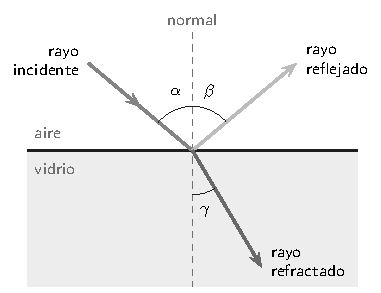
\includegraphics[max width=0.92\linewidth,max height=8.5cm]{fis/ond_reflex_refrac}
\end{center}
\altslargas{En el vidrio, la rapidez y la longitud de onda de la luz disminuyen, y su frecuencia se mantiene.}{El ángulo de reflexión $\beta$ es mayor que el ángulo de incidencia $\alpha$.}{El ángulo $\gamma$ es menor que $\alpha$ porque la frecuencia de la luz disminuye en el vidrio.}{El rayo reflejado tiene menor frecuencia que el rayo incidente.}
\solucion{\textbf{Paso 1. ¿Qué nos piden?} Una afirmación correcta sobre la reflexión y la refracción en la figura.

\textbf{Paso 2. Refracción.} El rayo refractado se acerca a la normal ($\gamma < \alpha$): la luz pasó a un medio donde va más lenta. Con la frecuencia constante, $\lambda = v/f$ también disminuye.

\textbf{Respuesta:} en el vidrio disminuyen la rapidez y la longitud de onda, y la frecuencia se mantiene.

\textbf{¿Por qué no las otras?} Por la ley de reflexión, $\beta = \alpha$. La frecuencia no cambia al refractarse: el rayo se acerca a la normal porque disminuye la rapidez. La reflexión tampoco cambia la frecuencia.

\textbf{\color{cienciaD}Para recordar.} Hacia el vidrio: menor rapidez y menor \ensuremath{\lambda}, misma frecuencia.}{A}
\end{elejemplo}

%% =====================================================================
%% fis_espejos_lentes
\section[Espejos y lentes]{Espejos y lentes}
\modcomun\ \ {\color{gris}\itshape Formación de imágenes en espejos planos, cóncavos y convexos y en lentes convergentes y divergentes: elementos (vértice, foco, centro de curvatura), rayos principales e imágenes reales o virtuales, derechas o invertidas, mayores o menores.\par}
\subsection{Imágenes y espejos planos}
Una \textbf{imagen} es el punto (o conjunto de puntos) desde donde parecen venir los rayos de luz después de reflejarse o refractarse.

 
\begin{itemize}
  \item \textbf{Imagen real:} los rayos realmente se cruzan en ella. Se puede \textbf{proyectar en una pantalla}.
  \item \textbf{Imagen virtual:} solo se cruzan las prolongaciones de los rayos. Se ve mirando el espejo o la lente, pero \textbf{no se puede proyectar}.
\end{itemize}
 

\textbf{Espejo plano.} La imagen es siempre:

 
\begin{itemize}
  \item \textbf{virtual} (está «detrás» del espejo);
  \item \textbf{derecha} (no se invierte de arriba a abajo);
  \item del \textbf{mismo tamaño} que el objeto;
  \item a la \textbf{misma distancia} del espejo que el objeto, pero detrás de él.
\end{itemize}
  
\begin{clave}[{Izquierda y derecha}] Si levantas tu mano derecha frente a un espejo, tu imagen levanta la mano que está a tu derecha, que para ella sería la izquierda. Por eso la palabra AMBULANCIA se escribe al revés en el capó: en el retrovisor del auto de adelante se lee bien.\end{clave}
 
\begin{clave}[{Recuerda}] Si estás a 2 m de un espejo plano, tu imagen está 2 m detrás del espejo: la distancia entre tú y tu imagen es 4 m.\end{clave}
\subsection{Espejos curvos: elementos y rayos principales}
Un \textbf{espejo cóncavo} refleja por su cara interior, como el interior de una cuchara; concentra la luz (es convergente). Un \textbf{espejo convexo} refleja por su cara exterior, como el dorso de una cuchara; dispersa la luz (es divergente).

 
\begin{itemize}
  \item \textbf{Vértice (V):} centro del espejo.
  \item \textbf{Eje óptico:} recta que pasa por el vértice y el centro de curvatura.
  \item \textbf{Centro de curvatura (C):} centro de la esfera de la que forma parte el espejo.
  \item \textbf{Foco (F):} punto medio entre C y V; en él se concentran los rayos que llegan paralelos al eje.
\end{itemize}
  

\textbf{Rayos principales en un espejo cóncavo} (basta dibujar dos para ubicar la imagen):

 
\begin{enumerate}
  \item Un rayo \textbf{paralelo al eje} se refleja pasando por el \textbf{foco}.
  \item Un rayo que pasa por el \textbf{foco} se refleja \textbf{paralelo al eje}.
  \item Un rayo que pasa por el \textbf{centro de curvatura} se refleja sobre sí mismo.
\end{enumerate}
 

En un espejo convexo, F y C están detrás del espejo: un rayo paralelo se refleja como si viniera del foco, y un rayo que apunta al foco se refleja paralelo.

 
\begin{clave}[{Recuerda}] Si pones una fuente de luz en el foco de un espejo cóncavo, los rayos salen paralelos: así funcionan los focos de los autos, las linternas y los faros.\end{clave}
\subsection{Imágenes en espejos cóncavos}
La imagen depende de dónde esté el objeto:

 
\begin{center}\small
\begin{tabular}{@{}ll@{}}
\toprule
\textbf{Posición del objeto} & \textbf{Imagen} \\
\midrule
más allá de C & real, invertida, menor \\
en C & real, invertida, de igual tamaño \\
entre C y F & real, invertida, mayor \\
en F & no se forma (los rayos salen paralelos) \\
entre F y V & virtual, derecha, mayor \\
\bottomrule
\end{tabular}
\end{center}
 

\textbf{Usos:} espejos de maquillaje y de dentista (la cara entre F y V: imagen derecha y aumentada), telescopios reflectores, focos y faros.

  
\begin{center}
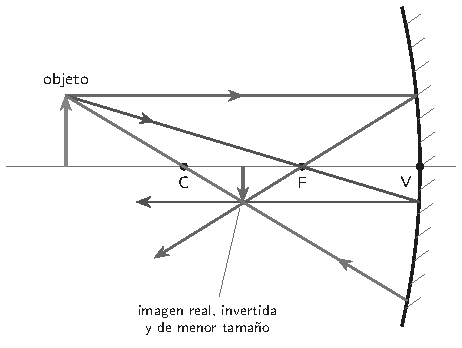
\includegraphics[max width=0.92\linewidth,max height=8.5cm]{fis/ond_espejo_concavo}
\end{center}
 
\begin{clave}[{Recuerda}] En un espejo cóncavo las imágenes reales son siempre invertidas; la única imagen derecha es la virtual, cuando el objeto está entre F y V.\end{clave}
\subsection{Espejos convexos}
En un espejo convexo, sin importar dónde esté el objeto, la imagen es siempre:

 
\begin{itemize}
  \item \textbf{virtual} (detrás del espejo, entre V y F),
  \item \textbf{derecha},
  \item de \textbf{menor tamaño} que el objeto.
\end{itemize}
 

Como las imágenes son más pequeñas, en el espejo cabe una zona mucho más amplia: tiene un gran \textbf{campo visual}.

 

\textbf{Usos:} espejos laterales de los autos, espejos de seguridad en tiendas, estacionamientos y curvas peligrosas.

 
\begin{clave}[{«Los objetos pueden estar más cerca de lo que aparentan»}] Esta advertencia aparece en los espejos laterales porque son convexos: la imagen es más pequeña que el objeto, y el cerebro interpreta que el objeto está más lejos.\end{clave}
  
\begin{center}
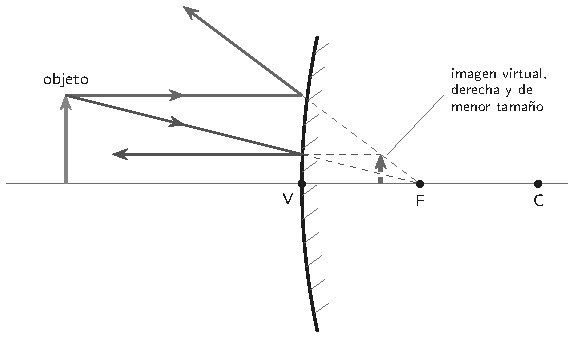
\includegraphics[max width=0.92\linewidth,max height=8.5cm]{fis/ond_espejo_convexo}
\end{center}
\subsection{Lentes convergentes}
Una lente \textbf{convergente} es más gruesa en el centro que en los bordes. Los rayos que llegan paralelos al eje se refractan y se juntan en el \textbf{foco} del otro lado. Tiene un foco a cada lado, a la misma distancia.

 

\textbf{Rayos principales:} (1) un rayo paralelo al eje sale pasando por el foco del otro lado; (2) un rayo que pasa por el centro de la lente no se desvía; (3) un rayo que pasa por el foco del lado del objeto sale paralelo al eje.

 
\begin{center}\small
\begin{tabularx}{\linewidth}{@{}>{\raggedright\arraybackslash\hsize=0.88\hsize}X>{\raggedright\arraybackslash\hsize=1.06\hsize}X>{\raggedright\arraybackslash\hsize=1.06\hsize}X@{}}
\toprule
\textbf{Posición del objeto} & \textbf{Imagen} & \textbf{Uso} \\
\midrule
más allá de 2F & real, invertida, menor & cámara fotográfica, ojo \\
en 2F & real, invertida, igual & fotocopiadora \\
entre 2F y F & real, invertida, mayor & proyector \\
en F & no se forma & linterna, faro \\
entre F y la lente & virtual, derecha, mayor & lupa \\
\bottomrule
\end{tabularx}
\end{center}
  
\begin{center}
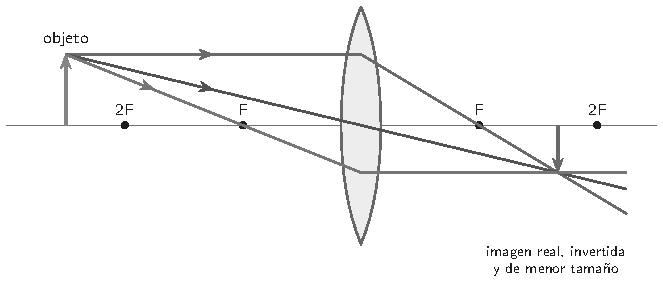
\includegraphics[max width=0.92\linewidth,max height=8.5cm]{fis/ond_lente_conv}
\end{center}
 
\begin{clave}[{Recuerda}] Las lentes convergentes se usan para corregir la \textbf{hipermetropía}.\end{clave}
\subsection{Lentes divergentes}
Una lente \textbf{divergente} es más delgada en el centro que en los bordes. Los rayos que llegan paralelos al eje se separan al atravesarla, como si vinieran del foco ubicado del lado del objeto.

 

Sin importar la posición del objeto, la imagen es siempre \textbf{virtual, derecha y de menor tamaño}, y está del mismo lado que el objeto, entre el foco y la lente.

 

\textbf{Usos:} mirillas de las puertas (dan una vista amplia), lentes para corregir la \textbf{miopía}, combinadas con lentes convergentes en cámaras y telescopios.

 
\begin{clave}[{Paralelo con los espejos}] · Espejo cóncavo y lente convergente: imágenes reales o virtuales según la posición.\par · Espejo convexo y lente divergente: siempre virtual, derecha y menor.\end{clave}
  
\begin{center}
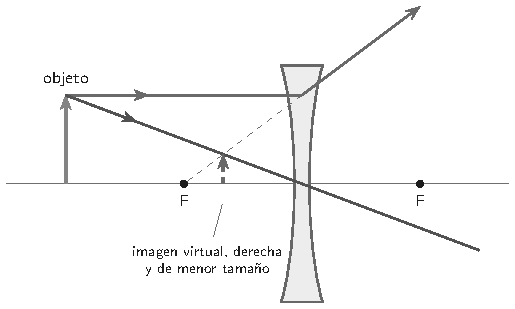
\includegraphics[max width=0.92\linewidth,max height=8.5cm]{fis/ond_lente_div}
\end{center}
\subsection{Lo clave del tema}
\begin{center}\small
\begin{tabularx}{\linewidth}{@{}>{\raggedright\arraybackslash\hsize=0.54\hsize}X>{\raggedright\arraybackslash\hsize=1.26\hsize}X>{\raggedright\arraybackslash\hsize=1.20\hsize}X@{}}
\toprule
\textbf{Elemento} & \textbf{Tipo de imagen} & \textbf{Usos típicos} \\
\midrule
Espejo plano & virtual, derecha, igual tamaño, a la misma distancia & espejos de baño, retrovisor interior \\
Espejo cóncavo & real e invertida (objeto más allá de F) o virtual, derecha y mayor (objeto entre F y V) & maquillaje, faros, telescopios \\
Espejo convexo & siempre virtual, derecha y menor & espejos laterales, seguridad \\
Lente convergente & real e invertida (objeto más allá de F) o virtual, derecha y mayor (objeto entre F y la lente) & lupa, proyector, cámara, hipermetropía \\
Lente divergente & siempre virtual, derecha y menor & mirillas, miopía \\
\bottomrule
\end{tabularx}
\end{center}
 
\begin{clave}[{Recuerda}] · Real = se proyecta en pantalla = invertida. Virtual = no se proyecta = derecha.\par · Con el objeto en el foco no se forma imagen: los rayos salen paralelos.\par · Paralelo al eje \ensuremath{\rightarrow} por el foco; por el foco \ensuremath{\rightarrow} paralelo al eje.\end{clave}
 
\begin{clave}[{Método PAES}] 1. Identifica el elemento (plano, cóncavo, convexo, convergente, divergente). 2. Si es convexo o divergente, la imagen es virtual, derecha y menor. 3. Si es cóncavo o convergente, ubica el objeto respecto de F y de C (o 2F) y usa la tabla. 4. En diagramas, verifica cada rayo con las reglas de los rayos principales.\end{clave}
\begin{elejemplo}{PAES Invierno 2027, adaptada}
Un joven viaja de copiloto en un furgón escolar y nota que el espejo lateral tiene escrita la advertencia «los objetos pueden estar más cerca de lo que aparentan». Le pregunta a la conductora, quien le explica correctamente usando lo que recuerda de física.

¿Cuál pudo ser la respuesta de la conductora?
\altslargas{Que al ser un espejo cóncavo, la imagen formada es invertida y de menor tamaño que los objetos.}{Que al ser un espejo cóncavo, la imagen formada es derecha y de mayor tamaño que los objetos.}{Que al ser un espejo convexo, la imagen formada es derecha y de menor tamaño que los objetos.}{Que al ser un espejo convexo, la imagen formada es invertida y de mayor tamaño que los objetos.}
\solucion{\textbf{Paso 1. ¿Qué nos piden?} Qué tipo de espejo produce la ilusión de que los objetos están más lejos.

\textbf{Paso 2. Piensa en el tamaño.} Si un objeto se ve más pequeño de lo normal, el cerebro interpreta que está más lejos. El espejo lateral debe formar imágenes más pequeñas que los objetos.

\textbf{Paso 3. Elige el espejo.} El espejo convexo forma siempre imágenes virtuales, derechas y menores, y además tiene un campo visual amplio.

\textbf{Respuesta:} es un espejo convexo y la imagen es derecha y de menor tamaño.

\textbf{¿Por qué no las otras?} Una imagen invertida haría ver los autos de cabeza, y un espejo lateral no hace eso. Una imagen mayor haría ver los objetos más cerca, no más lejos. Un espejo convexo nunca forma imágenes invertidas ni mayores.

\textbf{\color{cienciaD}Para recordar.} Espejo convexo: imagen virtual, derecha y menor; los objetos parecen más lejos.}{C}
\end{elejemplo}

%% =====================================================================
%% fis_dispositivos
\section[Dispositivos tecnológicos con ondas]{Dispositivos tecnológicos con ondas}
\modcomun\ \ {\color{gris}\itshape Cómo funcionan y para qué sirven la radio, la televisión, el teléfono móvil y la comunicación inalámbrica, el radar, los radiotelescopios, los telescopios reflector y refractor, los prismáticos, la fibra óptica y el láser.\par}
\subsection{Comunicación inalámbrica}
La radio, la televisión abierta, el teléfono móvil, el wifi, el bluetooth y el GPS transmiten información con \textbf{ondas de radio y microondas}. Todos siguen el mismo esquema:

 
\begin{enumerate}
  \item Un \textbf{emisor} convierte la información (sonido, imagen, datos) en una señal eléctrica.
  \item Una \textbf{antena emisora} la transforma en ondas electromagnéticas de una frecuencia determinada.
  \item Las ondas viajan a $3{,}0\times10^{8}$ m/s y llegan a una \textbf{antena receptora}.
  \item El \textbf{receptor} sintoniza esa frecuencia y recupera la información.
\end{enumerate}
 

La información se «monta» sobre la onda variando su amplitud (\textbf{AM}, amplitud modulada) o su frecuencia (\textbf{FM}, frecuencia modulada). Cada emisora tiene su propia frecuencia, para que las señales no se mezclen.

  
\begin{clave}[{Teléfono móvil}] El celular se comunica por microondas con la antena más cercana. El territorio se divide en zonas llamadas \textbf{celdas}, cada una con su antena; al moverte, la llamada pasa de una antena a otra. Las antenas se conectan entre sí por cables, fibra óptica o enlaces de microondas.\end{clave}
 
\begin{clave}[{Satélites}] Los satélites de comunicaciones reciben microondas desde la Tierra y las reenvían a otro punto. Permiten la televisión satelital, el GPS y las llamadas a lugares remotos.\end{clave}
\subsection{Radar y radiotelescopios}
\textbf{Radar.} Emite pulsos de microondas que se \textbf{propagan}, se \textbf{reflejan} en un objeto (avión, barco, nube de lluvia) y vuelven a la antena.

 

El \textbf{tiempo} de ida y vuelta da la distancia: la onda recorre dos veces la distancia, así que $d = \dfrac{c\,t}{2}$.

 

\textbf{Ejemplo.} Si un pulso vuelve $2{,}0\times10^{-4}$ s después de emitido: $d = \dfrac{3{,}0\times10^{8}\cdot 2{,}0\times10^{-4}}{2} = 3{,}0\times10^{4}$ m $= 30$ km.

 

Se usa en aeronáutica, navegación y meteorología.

  

\textbf{Radiotelescopios.} Grandes antenas parabólicas que captan las \textbf{ondas de radio} que emiten estrellas, galaxias y nubes de gas. La superficie parabólica refleja las ondas y las concentra en su \textbf{foco}, donde está el receptor. Pueden funcionar de día y a través de nubes.

 
\begin{clave}[{Chile y la astronomía}] El observatorio ALMA, en el llano de Chajnantor (Atacama), a unos 5000 m de altura, combina 66 antenas que captan ondas milimétricas. Se instaló allí porque el aire es muy seco: el vapor de agua absorbe esas ondas.\end{clave}
\subsection{Telescopios y prismáticos}
\textbf{Telescopio refractor.} Usa \textbf{lentes}. Una lente convergente grande (el \textbf{objetivo}) forma una imagen real del objeto lejano, y una segunda lente (el \textbf{ocular}) la amplía como una lupa. Así funcionaba el telescopio de Galileo.

 

\textbf{Telescopio reflector.} Usa un \textbf{espejo cóncavo} (el espejo primario) para reunir la luz y formar la imagen; un espejo secundario la dirige al ocular o a la cámara. Lo diseñó Newton.

 

Los grandes telescopios actuales, como los de Paranal o el ELT en el norte de Chile, son \textbf{reflectores}: un espejo se puede fabricar mucho más grande que una lente y sostenerse por detrás, sin deformarse.

  

\textbf{Prismáticos (binoculares).} Son dos pequeños telescopios refractores, uno para cada ojo. Entre el objetivo y el ocular tienen \textbf{prismas} que reflejan la luz varias veces por \textbf{reflexión total interna}. Los prismas cumplen dos funciones:

 
\begin{itemize}
  \item \textbf{enderezan} la imagen, que el objetivo forma invertida;
  \item \textbf{acortan} el instrumento, porque la luz recorre el camino en zigzag.
\end{itemize}
 
\begin{clave}[{Recuerda}] Mientras mayor es el objetivo (lente o espejo), más luz reúne el telescopio y más débiles son los objetos que puede observar.\end{clave}
\subsection{Fibra óptica}
Una \textbf{fibra óptica} es un hilo muy delgado de vidrio o plástico formado por un \textbf{núcleo}, con mayor índice de refracción, rodeado por un \textbf{revestimiento}, con menor índice.

 

La luz entra por un extremo y, cada vez que llega al límite entre el núcleo y el revestimiento con un ángulo mayor que el ángulo límite, se refleja por completo: \textbf{reflexión total interna}. Así avanza en zigzag por la fibra, aunque esta se curve, y casi sin perder intensidad.

 

\textbf{Usos:} internet y telefonía de alta velocidad (la información viaja como pulsos de luz, normalmente infrarroja), endoscopios médicos que permiten ver el interior del cuerpo, iluminación decorativa.

  
\begin{center}
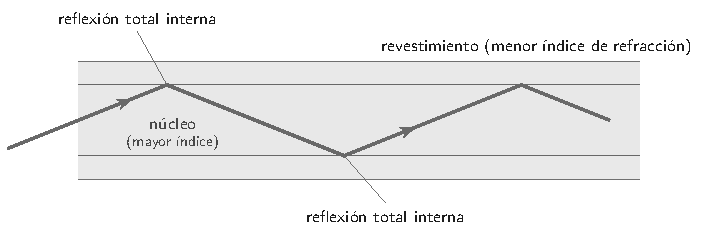
\includegraphics[max width=0.92\linewidth,max height=8.5cm]{fis/ond_fibra}
\end{center}
 
\begin{clave}[{Recuerda}] La reflexión total interna solo ocurre cuando la luz va de un medio donde es más lenta (mayor índice) a uno donde es más rápida (menor índice). Por eso el núcleo debe tener mayor índice que el revestimiento.\end{clave}
\subsection{Láser, pantallas y controles remotos}
\textbf{Láser.} Produce una luz con tres propiedades especiales:

 
\begin{itemize}
  \item \textbf{monocromática:} de una sola frecuencia (un solo color);
  \item \textbf{coherente:} todas sus ondas oscilan en fase;
  \item \textbf{direccional:} el haz casi no se abre, y concentra mucha energía en un punto pequeño.
\end{itemize}
 

\textbf{Usos:} lectores de códigos de barras, medición de distancias, cirugías y tratamientos oculares, corte de materiales, punteros, comunicación por fibra óptica, experimentos de interferencia.

  

\textbf{Televisor y pantallas.} La pantalla está formada por millones de \textbf{píxeles}, cada uno con puntos rojo, verde y azul. Encendiéndolos con distinta intensidad se obtiene cualquier color por \textbf{mezcla aditiva}: rojo y verde dan amarillo; los tres juntos, blanco.

 

\textbf{Control remoto.} Envía pulsos de \textbf{luz infrarroja} que el televisor detecta. Como el infrarrojo no atraviesa objetos opacos, hay que apuntar al televisor sin obstáculos. El wifi, en cambio, usa microondas, que atraviesan en buena medida paredes y muebles.

 
\begin{clave}[{Recuerda}] La cámara de un celular puede ver el destello infrarrojo de un control remoto, aunque tus ojos no lo vean.\end{clave}
\subsection{Lo clave del tema}
\begin{center}\small
\begin{tabularx}{\linewidth}{@{}>{\raggedright\arraybackslash\hsize=1.04\hsize}X>{\raggedright\arraybackslash\hsize=0.73\hsize}X>{\raggedright\arraybackslash\hsize=1.22\hsize}X@{}}
\toprule
\textbf{Dispositivo} & \textbf{Onda que usa} & \textbf{Fenómeno o principio} \\
\midrule
Radio, TV, celular, wifi & radio y microondas & emisión y recepción por antenas; cada señal con su frecuencia \\
Radar & microondas & propagación y reflexión; $d = ct/2$ \\
Radiotelescopio, antena parabólica & radio y microondas & reflexión en una superficie parabólica que concentra en el foco \\
Telescopio refractor & luz visible & refracción en lentes convergentes \\
Telescopio reflector & luz visible e infrarroja & reflexión en un espejo cóncavo \\
Prismáticos & luz visible & lentes y prismas con reflexión total interna \\
Fibra óptica & luz visible e infrarroja & reflexión total interna \\
Láser & luz de una frecuencia & haz monocromático, coherente y direccional \\
Control remoto, cámara térmica & infrarrojo & emisión y detección de infrarrojo \\
\bottomrule
\end{tabularx}
\end{center}
 
\begin{clave}[{Método PAES}] 1. Identifica qué onda usa el dispositivo y ubícala en el espectro. 2. Pregúntate qué le pasa a la onda: se propaga, se refleja, se refracta o se absorbe. 3. En cálculos de radar o comunicación, usa $d = v\,t$ y recuerda si el viaje es de ida o de ida y vuelta.\end{clave}
\begin{elejemplo}{PAES Invierno 2026, adaptada}
El radar se usa ampliamente en aeronáutica, navegación y meteorología, porque permite determinar la posición de objetos y seguir sus trayectorias.

¿Qué fenómenos asociados a las ondas electromagnéticas explican el funcionamiento del radar?
\alts{La difracción y la absorción.}{La refracción y la absorción.}{La propagación y la difracción.}{La propagación y la reflexión.}
\solucion{\textbf{Paso 1. ¿Qué nos piden?} Los fenómenos en que se basa el radar.

\textbf{Paso 2. Sigue la onda.} El radar emite microondas que viajan por el aire hasta el objeto (\textbf{propagación}), rebotan en él (\textbf{reflexión}) y vuelven a la antena. Midiendo el tiempo de ida y vuelta calcula la distancia.

\textbf{Respuesta:} la propagación y la reflexión.

\textbf{¿Por qué no las otras?} Si el objeto absorbiera las microondas, no volvería señal al radar. La refracción y la difracción pueden ocurrir, pero no son la base del funcionamiento: lo esencial es que la onda vaya y vuelva reflejada.

\textbf{\color{cienciaD}Para recordar.} Radar: la onda viaja, se refleja en el objeto y vuelve.}{D}
\end{elejemplo}

\chapter{Mecánica}
%% =====================================================================
%% fis_cinematica
\section[Describir el movimiento]{Describir el movimiento}
\modcomun\ \ {\color{gris}\itshape Sistema de referencia, trayectoria y posición; distancia recorrida frente a desplazamiento; rapidez media frente a velocidad media; velocidad instantánea y aceleración; y relatividad de Galileo con suma de velocidades (trenes, ríos y escaleras mecánicas).\par}
\subsection{Sistema de referencia, posición y trayectoria}
Para describir un movimiento primero se elige un \textbf{sistema de referencia}: un punto de origen, un eje con un sentido positivo y un reloj para medir el tiempo.

 

La \textbf{posición} ($x$) indica dónde está el cuerpo respecto del origen. En una línea recta basta un número con signo: $x = +3$ m está 3 m hacia el lado positivo del origen y $x = -2$ m está 2 m hacia el lado negativo.

 

La \textbf{trayectoria} es la línea que describe el cuerpo al moverse: recta, curva, circular.

 

El \textbf{tiempo transcurrido} entre dos instantes es $\Delta t = t_f - t_i$.

  
\begin{clave}[{El movimiento es relativo}] Un pasajero sentado en un bus está en reposo respecto del bus y en movimiento respecto de la calle. Antes de decir «se mueve» o «está quieto», pregúntate: ¿respecto de qué?\end{clave}
 
\begin{clave}[{Recuerda}] La posición depende del origen que se elija. En cambio, el cambio de posición entre dos instantes es el mismo para dos observadores quietos uno respecto del otro, aunque usen orígenes distintos.\end{clave}
\subsection{Distancia recorrida y desplazamiento}
El \textbf{desplazamiento} es el cambio de posición: \[ \Delta x = x_f - x_i \] Tiene magnitud, dirección y sentido (es un vector). En una recta, su signo indica el sentido.

 

La \textbf{distancia recorrida} ($d$) es el largo total del camino seguido. Siempre es positiva y nunca disminuye mientras el cuerpo se mueve.

 

En la figura, un carrito parte en $x = 2$ m, avanza hasta $x = 10$ m y regresa hasta $x = 6$ m:

 
\begin{itemize}
  \item distancia recorrida: $d = 8 + 4 = 12$ m;
  \item desplazamiento: $\Delta x = 6 - 2 = +4$ m.
\end{itemize}
  
\begin{center}
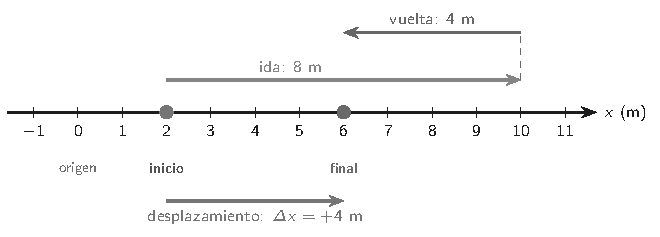
\includegraphics[max width=0.92\linewidth,max height=8.5cm]{fis/mov_trayecto}
\end{center}
 
\begin{clave}[{Recuerda}] La distancia recorrida coincide con la magnitud del desplazamiento solo si el cuerpo se mueve en línea recta sin devolverse. Si vuelve al punto de partida, su desplazamiento es nulo, aunque haya recorrido mucho.\end{clave}
\subsection{Rapidez media y velocidad media}
La \textbf{rapidez media} compara la distancia recorrida con el tiempo empleado:

 
\begin{center}
$\text{rapidez media} = \dfrac{d}{\Delta t}$
\end{center}
 

La \textbf{velocidad media} compara el desplazamiento con el tiempo, y tiene el sentido del desplazamiento:

 
\begin{center}
$v_m = \dfrac{\Delta x}{\Delta t}$
\end{center}
 

\textbf{Ejemplo.} Una persona camina 300 m hacia el este y luego 100 m hacia el oeste, en un total de 200 s. Recorre $d = 400$ m y su desplazamiento es 200 m hacia el este. Su rapidez media es $\dfrac{400}{200} = 2$ m/s y su velocidad media es $\dfrac{200}{200} = 1$ m/s hacia el este.

  
\begin{clave}[{Unidades}] En el SI la rapidez y la velocidad se miden en m/s. Para pasar de km/h a m/s se divide por 3,6: $72$ km/h $= 20$ m/s y $36$ km/h $= 10$ m/s.\end{clave}
 
\begin{clave}[{Recuerda}] La rapidez media no es el promedio de las rapideces. Si recorres 30 km a 60 km/h (0,5 h) y otros 30 km a 30 km/h (1 h), tu rapidez media es $\dfrac{60}{1{,}5} = 40$ km/h, no 45 km/h. Siempre divide la distancia total por el tiempo total, incluidas las detenciones.\end{clave}
\subsection{Velocidad instantánea y aceleración}
La \textbf{velocidad instantánea} es la velocidad en un instante determinado. Su magnitud, la \textbf{rapidez instantánea}, es lo que marca el velocímetro de un auto.

 

La \textbf{aceleración} mide qué tan rápido cambia la velocidad:

 
\begin{center}
$a = \dfrac{\Delta v}{\Delta t} = \dfrac{v_f - v_i}{\Delta t}$
\end{center}
 

Su unidad es m/s². Si un auto pasa de 5 m/s a 25 m/s en 4 s, su aceleración es $a = \dfrac{25 - 5}{4} = 5$ m/s²: cada segundo su velocidad aumenta 5 m/s.

 

En una recta, si la aceleración y la velocidad tienen el \textbf{mismo signo}, la rapidez aumenta; si tienen \textbf{signos opuestos}, la rapidez disminuye (el cuerpo frena).

  
\begin{clave}[{Hay aceleración siempre que cambie la velocidad}] · si aumenta la rapidez;\par · si disminuye la rapidez (frenar también es acelerar);\par · si cambia la dirección, aunque la rapidez sea constante, como un auto que toma una curva con el velocímetro fijo.\end{clave}
 
\begin{clave}[{Recuerda}] Velocidad y aceleración son magnitudes distintas. Una pelota lanzada hacia arriba tiene velocidad nula en el punto más alto y, sin embargo, su aceleración es la de gravedad. Un avión en vuelo recto a velocidad constante tiene gran velocidad y aceleración nula.\end{clave}
\subsection{Relatividad de Galileo}
Galileo observó que dentro de un barco que navega con velocidad constante y sin sacudidas, una pelota cae, rueda y rebota igual que en tierra firme. Ningún experimento mecánico hecho dentro del barco permite saber si se mueve. Las leyes del movimiento son las mismas en todos los sistemas de referencia que se mueven con \textbf{velocidad constante} unos respecto de otros.

 

Lo que sí cambia de un observador a otro son las \textbf{posiciones, las velocidades y las trayectorias}. Para movimientos sobre una misma recta, las velocidades se suman con su signo:

 
\begin{center}
$v_{\text{respecto del suelo}} = v_{\text{respecto del tren}} + v_{\text{tren}}$
\end{center}
 
\begin{itemize}
  \item Tren a 15 m/s y pasajero que camina hacia adelante a 2 m/s: 17 m/s respecto del andén. Si camina hacia atrás: $15 - 2 = 13$ m/s.
  \item Bote a 5 m/s respecto del agua en un río que fluye a 2 m/s: 7 m/s río abajo y 3 m/s río arriba, respecto de la orilla.
\end{itemize}
  
\begin{center}
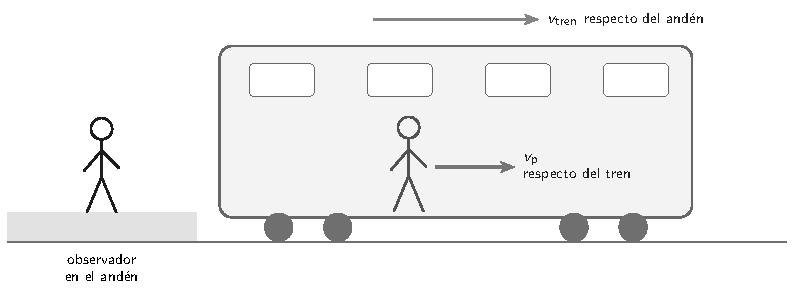
\includegraphics[max width=0.92\linewidth,max height=8.5cm]{fis/mov_tren}
\end{center}
 
\begin{clave}[{Recuerda}] Si un pasajero suelta una moneda en un tren que avanza a velocidad constante, para él la moneda cae en línea recta vertical. Para una persona en el andén, la moneda también avanza junto con el tren y describe una curva. La trayectoria depende del sistema de referencia.\end{clave}
\subsection{Lo clave del tema}
\begin{center}\small
\begin{tabularx}{\linewidth}{@{}>{\raggedright\arraybackslash\hsize=0.76\hsize}X>{\raggedright\arraybackslash\hsize=1.60\hsize}X>{\raggedright\arraybackslash\hsize=1.28\hsize}X>{\raggedright\arraybackslash\hsize=0.36\hsize}X@{}}
\toprule
\textbf{Magnitud} & \textbf{Qué es} & \textbf{Cómo se calcula} & \textbf{Unidad SI} \\
\midrule
Posición & dónde está respecto del origen & $x$ & m \\
Desplazamiento & cambio de posición, con sentido & $\Delta x = x_f - x_i$ & m \\
Distancia recorrida & largo total del camino & suma de los tramos & m \\
Rapidez media & distancia por unidad de tiempo & $d / \Delta t$ & m/s \\
Velocidad media & desplazamiento por unidad de tiempo & $\Delta x / \Delta t$ & m/s \\
Aceleración & cambio de velocidad por unidad de tiempo & $\Delta v / \Delta t$ & m/s² \\
Velocidad relativa & velocidad vista desde otro sistema & en una recta, se suman con signo & m/s \\
\bottomrule
\end{tabularx}
\end{center}
 
\begin{clave}[{Recuerda}] · Si el cuerpo vuelve al punto de partida, su desplazamiento y su velocidad media son nulos.\par · La rapidez media usa el tiempo total, incluidas las detenciones.\par · Frenar y doblar también son formas de acelerar.\par · Posición, velocidad y trayectoria dependen del observador; las leyes del movimiento son las mismas para observadores con velocidad constante entre sí.\end{clave}
 
\begin{clave}[{Método PAES}] 1. Fija el origen y el sentido positivo. 2. Distingue si te piden algo escalar (distancia, rapidez) o vectorial (desplazamiento, velocidad). 3. Usa siempre totales: distancia total y tiempo total. 4. Revisa las unidades (km/h o m/s). 5. En problemas de trenes, ríos o escaleras, pregunta respecto de quién se da cada velocidad antes de sumar.\end{clave}
\begin{elejemplo}{Estilo PAES}
Un carrito de juguete se mueve sobre una pista recta. La figura muestra su recorrido: parte en $x = 2$ m, avanza hasta $x = 10$ m y luego regresa hasta $x = 6$ m. Todo el recorrido dura 4 s.

¿Cuáles son, respectivamente, la rapidez media del carrito y la magnitud de su velocidad media en esos 4 s?
\begin{center}
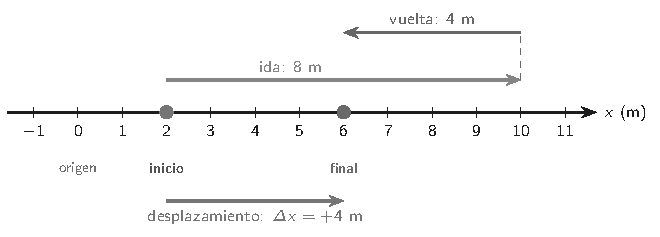
\includegraphics[max width=0.92\linewidth,max height=8.5cm]{fis/mov_trayecto}
\end{center}
\alts{1 m/s y 3 m/s}{3 m/s y 3 m/s}{3 m/s y 1 m/s}{1,5 m/s y 1 m/s}
\solucion{\textbf{Paso 1. ¿Qué nos piden?} Dos magnitudes distintas: la rapidez media, que usa la distancia recorrida, y la velocidad media, que usa el desplazamiento.

\textbf{Paso 2. Distancia recorrida.} Ida de 2 m a 10 m: 8 m. Vuelta de 10 m a 6 m: 4 m. Total: $d = 12$ m.

\textbf{Paso 3. Desplazamiento.} Solo importan la posición final y la inicial: $\Delta x = 6 - 2 = +4$ m.

\textbf{Paso 4. Divide por el tiempo total.} Rapidez media $= \dfrac{12}{4} = 3$ m/s. Velocidad media $= \dfrac{4}{4} = 1$ m/s.

\textbf{Respuesta:} 3 m/s y 1 m/s.

\textbf{¿Por qué no las otras?} «1 m/s y 3 m/s» intercambia las dos magnitudes. «3 m/s y 3 m/s» usa la distancia recorrida también para la velocidad media. «1,5 m/s y 1 m/s» divide la posición final (6 m) por el tiempo, en lugar de la distancia recorrida.

\textbf{\color{cienciaD}Para recordar.} Rapidez media: distancia total / tiempo. Velocidad media: desplazamiento / tiempo.}{C}
\end{elejemplo}

%% =====================================================================
%% fis_mru
\section[Movimiento rectilíneo uniforme]{Movimiento rectilíneo uniforme}
\modcomun\ \ {\color{gris}\itshape Movimiento en línea recta con velocidad constante: ecuación de itinerario x(t) = x0 + v t, lectura de gráficos posición--tiempo (pendiente) y velocidad--tiempo (área), y problemas de encuentro y alcance entre dos móviles.\par}
\subsection{El movimiento rectilíneo uniforme}
Un cuerpo tiene \textbf{movimiento rectilíneo uniforme (MRU)} cuando se mueve en línea recta con \textbf{velocidad constante}: misma rapidez y mismo sentido todo el tiempo. Recorre \textbf{distancias iguales en tiempos iguales} y su aceleración es nula.

 

La \textbf{ecuación de itinerario} entrega la posición en cada instante:

 
\begin{center}
$x(t) = x_0 + v\,t$
\end{center}
 

$x_0$ es la posición inicial (en $t = 0$) y $v$ es la velocidad, con signo: positiva si el cuerpo avanza en el sentido del eje, negativa si avanza en sentido contrario.

 
\begin{itemize}
  \item $x(t) = 5 + 3t$: parte en 5 m y avanza 3 m cada segundo. A los 4 s está en $5 + 12 = 17$ m.
  \item $x(t) = 20 - 4t$: parte en 20 m y se mueve en sentido negativo a 4 m/s. Pasa por el origen cuando $20 - 4t = 0$, es decir, a los 5 s.
\end{itemize}
  
\begin{clave}[{Recuerda}] De la ecuación se obtienen las relaciones de siempre: $\Delta x = v\,t$, $\;t = \dfrac{\Delta x}{v}$, $\;v = \dfrac{\Delta x}{t}$. Usa unidades coherentes: metros con segundos, o kilómetros con horas.\end{clave}
 
\begin{ejemplo}[{Ejemplos de MRU}] La luz viaja en el vacío a $3{,}0\times10^8$ m/s y el sonido en el aire a unos 340 m/s. Por eso, en una tormenta, primero se ve el relámpago y después se oye el trueno.\end{ejemplo}
\subsection{Gráfico posición--tiempo}
En un MRU, el gráfico $x$--$t$ es una \textbf{recta}:

 
\begin{itemize}
  \item donde la recta corta el eje vertical se lee la posición inicial $x_0$;
  \item la \textbf{pendiente} es la velocidad: $v = \dfrac{\Delta x}{\Delta t}$;
  \item recta que sube: velocidad positiva; recta que baja: velocidad negativa; recta horizontal: reposo;
  \item mientras más inclinada, mayor es la rapidez.
\end{itemize}
 

En la figura: A parte del origen con $v_A = \dfrac{32 - 0}{8} = 4$ m/s. B parte en 24 m con $v_B = \dfrac{0 - 24}{8} = -3$ m/s. C está en reposo en $x = 12$ m.

  
\begin{center}
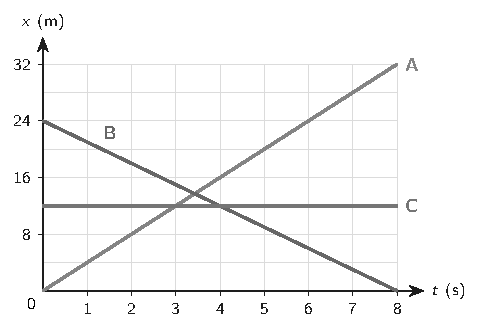
\includegraphics[max width=0.92\linewidth,max height=8.5cm]{fis/mov_mru_xt}
\end{center}
 
\begin{clave}[{Recuerda}] El gráfico $x$--$t$ no es un dibujo de la trayectoria. Una recta que baja no significa que el cuerpo baje por una pendiente: significa que se mueve en el sentido negativo del eje.\end{clave}
\subsection{Gráfico velocidad--tiempo}
En un MRU la velocidad no cambia: el gráfico $v$--$t$ es una \textbf{recta horizontal} a la altura de la velocidad.

 

El \textbf{área} entre esa recta y el eje del tiempo es el \textbf{desplazamiento}: $\Delta x = v\,\Delta t$. En la figura, $v = 5$ m/s durante 6 s: área $= 5\cdot 6 = 30$ m.

 

Si la velocidad es negativa, la recta queda bajo el eje y su área cuenta como desplazamiento negativo. La distancia recorrida suma todas las áreas como positivas.

 

El gráfico aceleración--tiempo de un MRU coincide con el eje del tiempo: $a = 0$.

  
\begin{center}
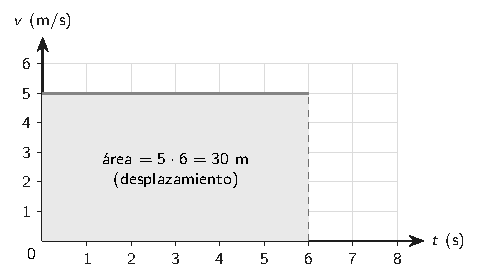
\includegraphics[max width=0.92\linewidth,max height=8.5cm]{fis/mov_mru_vt}
\end{center}
 
\begin{clave}[{Recuerda}] En el gráfico $x$--$t$ se mira la pendiente. En el gráfico $v$--$t$ se mira la altura (la velocidad) y el área (el desplazamiento). Antes de responder, lee qué magnitud hay en cada eje.\end{clave}
\subsection{Encuentros y alcances}
Dos móviles que van por la misma recta se \textbf{encuentran} en el instante en que tienen la \textbf{misma posición}. Método:

 
\begin{enumerate}
  \item Elige un único origen y un único sentido positivo para ambos.
  \item Escribe la ecuación de itinerario de cada uno.
  \item Iguala $x_A(t) = x_B(t)$ y despeja $t$.
  \item Reemplaza ese $t$ en cualquiera de las ecuaciones para saber dónde se encuentran.
\end{enumerate}
 

\textbf{Atajo.} Si se mueven uno hacia el otro, la distancia $D$ que los separa disminuye con la suma de sus rapideces: $t = \dfrac{D}{v_A + v_B}$. Si uno persigue al otro, disminuye con la diferencia: $t = \dfrac{D}{v_A - v_B}$.

  
\begin{ejemplo}[{Ejemplo resuelto}] Un auto A pasa por $x = 0$ a 15 m/s persiguiendo a un camión B, que está en $x = 100$ m y avanza a 10 m/s en el mismo sentido.\par \textbf{Paso 1.} $x_A = 15t$ y $x_B = 100 + 10t$.\par \textbf{Paso 2.} $15t = 100 + 10t \Rightarrow 5t = 100 \Rightarrow t = 20$ s.\par \textbf{Paso 3.} $x_A = 15\cdot 20 = 300$ m. Comprobación: $x_B = 100 + 200 = 300$ m. \ding{52}\end{ejemplo}
 
\begin{clave}[{Recuerda}] En un gráfico $x$--$t$, el encuentro es el punto donde se cruzan las rectas. En un gráfico $v$--$t$, que dos rectas se crucen indica que los móviles tienen la misma velocidad en ese instante, no que se encuentren.\end{clave}
\subsection{Lo clave del tema}
\begin{center}\small
\begin{tabularx}{\linewidth}{@{}>{\raggedright\arraybackslash\hsize=0.65\hsize}X>{\raggedright\arraybackslash\hsize=1.18\hsize}X>{\raggedright\arraybackslash\hsize=1.18\hsize}X@{}}
\toprule
\textbf{Herramienta} & \textbf{Forma en un MRU} & \textbf{Qué se lee} \\
\midrule
Ecuación de itinerario & $x(t) = x_0 + v\,t$ & posición en cada instante \\
Gráfico $x$--$t$ & recta inclinada (horizontal si está en reposo) & $x_0$ en el eje vertical; pendiente = velocidad; cruce de rectas = encuentro \\
Gráfico $v$--$t$ & recta horizontal & altura = velocidad; área = desplazamiento \\
Gráfico $a$--$t$ & sobre el eje ($a = 0$) & no hay aceleración \\
Encuentro & $x_A(t) = x_B(t)$ & instante y lugar donde coinciden \\
\bottomrule
\end{tabularx}
\end{center}
 
\begin{clave}[{Recuerda}] · MRU: distancias iguales en tiempos iguales.\par · El signo de $v$ indica el sentido del movimiento, no si el cuerpo acelera.\par · La rapidez media de un viaje con tramos distintos no es un MRU: se calcula con totales.\par · Uno hacia el otro: se suman las rapideces; uno detrás del otro: se restan.\end{clave}
 
\begin{clave}[{Método PAES}] 1. Lee los ejes del gráfico y sus unidades. 2. En $x$--$t$, calcula pendientes; en $v$--$t$, calcula áreas. 3. En encuentros, usa un solo origen para los dos móviles. 4. Comprueba la respuesta reemplazando en ambas ecuaciones.\end{clave}
\begin{elejemplo}{Estilo PAES}
En una carretera recta, el auto A pasa por la posición $x = 0$ con una velocidad constante de 20 m/s hacia la derecha. En ese mismo instante, el auto B pasa por $x = 300$ m con una velocidad constante de 10 m/s hacia la izquierda, como muestra la figura.

¿En qué instante y a qué distancia de la posición inicial de A se encuentran los autos?
\begin{center}
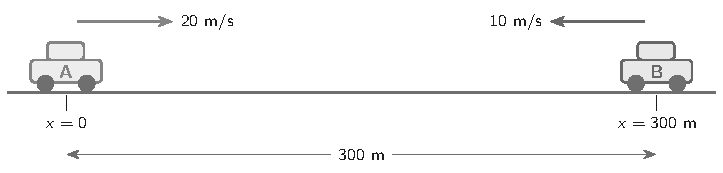
\includegraphics[max width=0.92\linewidth,max height=8.5cm]{fis/mov_encuentro}
\end{center}
\altslargas{A los 10 s, a 100 m de la posición inicial de A.}{A los 10 s, a 200 m de la posición inicial de A.}{A los 15 s, a 300 m de la posición inicial de A.}{A los 30 s, a 600 m de la posición inicial de A.}
\solucion{\textbf{Paso 1. ¿Qué nos piden?} El instante y la posición en que los dos autos coinciden.

\textbf{Paso 2. Ecuaciones de itinerario.} Con origen en la posición inicial de A y positivo hacia la derecha: $x_A = 20t$ y $x_B = 300 - 10t$ (B va en sentido negativo).

\textbf{Paso 3. Iguala.} $20t = 300 - 10t \Rightarrow 30t = 300 \Rightarrow t = 10$ s.

\textbf{Paso 4. Posición.} $x_A = 20\cdot 10 = 200$ m. Comprobación: $x_B = 300 - 100 = 200$ m. \ding{52}

\textbf{Respuesta:} a los 10 s, a 200 m de la posición inicial de A.

\textbf{¿Por qué no las otras?} 100 m es la distancia que recorre B, no la posición del encuentro medida desde A. 15 s es el tiempo que tardaría A en llegar a 300 m si B estuviera detenido. 30 s resta las rapideces, como si B fuera en el mismo sentido que A.

\textbf{\color{cienciaD}Para recordar.} Encuentro: iguala las ecuaciones de itinerario con un solo origen para ambos móviles.}{B}
\end{elejemplo}

%% =====================================================================
%% fis_mrua
\section[Movimiento rectilíneo uniformemente acelerado]{Movimiento rectilíneo uniformemente acelerado}
\modcomun\ \ {\color{gris}\itshape Movimiento en línea recta con aceleración constante: ecuaciones v(t) = v0 + a t y x(t) = x0 + v0 t + ½ a t², gráficos x--t (parábola), v--t (pendiente y área) y a--t, caída libre y lanzamiento vertical con g = 10 m/s², y distancia de frenado.\par}
\subsection{Movimiento con aceleración constante}
Un cuerpo tiene \textbf{movimiento rectilíneo uniformemente acelerado (MRUA)} cuando se mueve en línea recta con \textbf{aceleración constante}: su velocidad cambia en la misma cantidad cada segundo.

 
\begin{center}
$v(t) = v_0 + a\,t$
\end{center}
 

Por ejemplo, un auto que parte del reposo con $a = 2$ m/s²:

 
\begin{center}\small
\begin{tabular}{@{}llllll@{}}
\toprule
\textbf{$t$ (s)} & \textbf{0} & \textbf{1} & \textbf{2} & \textbf{3} & \textbf{4} \\
\midrule
\textbf{$v$ (m/s)} & 0 & 2 & 4 & 6 & 8 \\
\bottomrule
\end{tabular}
\end{center}
 

Si $a$ y $v$ tienen el \textbf{mismo signo}, la rapidez aumenta. Si tienen \textbf{signos opuestos}, la rapidez disminuye: el cuerpo frena hasta detenerse y, si la aceleración sigue actuando, empieza a moverse en sentido contrario.

  
\begin{clave}[{Recuerda}] Frenar no siempre significa aceleración negativa: significa que la aceleración y la velocidad tienen signos opuestos. Un auto que retrocede ($v < 0$) y frena tiene aceleración positiva.\end{clave}
 
\begin{clave}[{Recuerda}] La aceleración de un MRUA es constante, pero su velocidad cambia. Si un problema dice «parte del reposo», entonces $v_0 = 0$; si dice «se detiene», entonces la velocidad final es 0.\end{clave}
\subsection{Ecuación de itinerario del MRUA}
La posición en cada instante es:

 
\begin{center}
$x(t) = x_0 + v_0\,t + \tfrac{1}{2}\,a\,t^2$
\end{center}
 

Si parte del reposo desde el origen, queda $x = \tfrac{1}{2}\,a\,t^2$. Con $a = 4$ m/s², en 3 s recorre $\tfrac{1}{2}\cdot 4\cdot 9 = 18$ m.

 

Dos relaciones útiles que salen de las anteriores:

 
\begin{itemize}
  \item Velocidad media: $\Delta x = \dfrac{v_0 + v}{2}\,t$.
  \item Sin el tiempo: $v^2 = v_0^2 + 2\,a\,\Delta x$.
\end{itemize}
  
\begin{clave}[{Recuerda}] No olvides el $\tfrac{1}{2}$: en $x(t) = 5 + 2t + 3t^2$, el coeficiente de $t^2$ es $\tfrac{a}{2} = 3$, así que $a = 6$ m/s². Además, $x_0 = 5$ m y $v_0 = 2$ m/s.\end{clave}
 
\begin{clave}[{Distancias en segundos sucesivos}] Partiendo del reposo, lo que se recorre en el 1.º, 2.º, 3.º y 4.º segundo crece como 1 : 3 : 5 : 7. Con $a = 2$ m/s²: 1 m, 3 m, 5 m y 7 m. Si las distancias en intervalos iguales aumentan siempre en la misma cantidad, el movimiento es uniformemente acelerado.\end{clave}
\subsection{Gráficos del MRUA}
\begin{center}
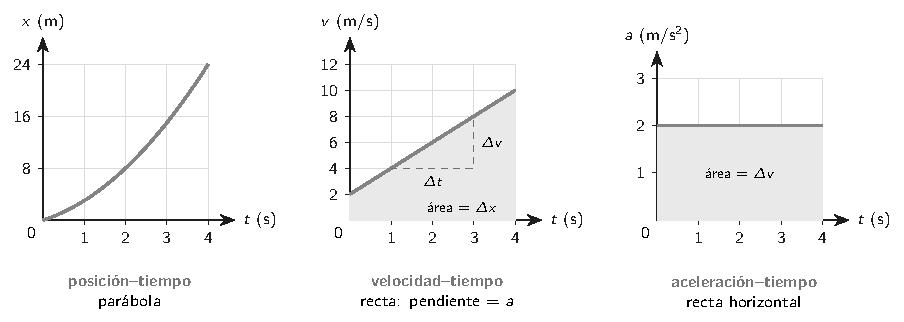
\includegraphics[max width=0.92\linewidth,max height=8.5cm]{fis/mov_mrua_graficos}
\end{center}
  

\textbf{$x$--$t$:} una \textbf{parábola}. Su pendiente, que es la velocidad, cambia: si la curva se empina, el cuerpo va cada vez más rápido.

 

\textbf{$v$--$t$:} una \textbf{recta inclinada}. Corta el eje vertical en $v_0$; su \textbf{pendiente es la aceleración}: $a = \dfrac{\Delta v}{\Delta t} = \dfrac{10 - 2}{4} = 2$ m/s².

  

El \textbf{área bajo $v$--$t$} es el desplazamiento. Aquí es un trapecio: $\Delta x = \dfrac{2 + 10}{2}\cdot 4 = 24$ m, igual que en el gráfico $x$--$t$.

 

\textbf{$a$--$t$:} una \textbf{recta horizontal}. El área bajo ella es el cambio de velocidad: $2\cdot 4 = 8$ m/s.
\subsection{Caída libre y lanzamiento vertical}
Si el roce con el aire es despreciable, todos los cuerpos caen con la misma aceleración, la \textbf{aceleración de gravedad}: $g = 10$ m/s², dirigida hacia abajo. No depende de la masa: un martillo y una pluma soltados en la Luna llegan al suelo al mismo tiempo.

 

Para un cuerpo que se suelta desde el reposo:

 
\begin{center}
$v = g\,t \qquad h = \tfrac{1}{2}\,g\,t^2$
\end{center}
 

\textbf{Lanzamiento hacia arriba.} El cuerpo sube cada vez más lento, se detiene un instante en el punto más alto y luego cae. Durante todo el movimiento su aceleración es $g$ hacia abajo, también en el punto más alto. Si se lanza con $v_0 = 20$ m/s:

 
\begin{itemize}
  \item tiempo de subida: $\dfrac{v_0}{g} = 2$ s, y otros 2 s de bajada;
  \item altura máxima: $\dfrac{v_0^2}{2g} = \dfrac{400}{20} = 20$ m.
\end{itemize}
  
\begin{center}
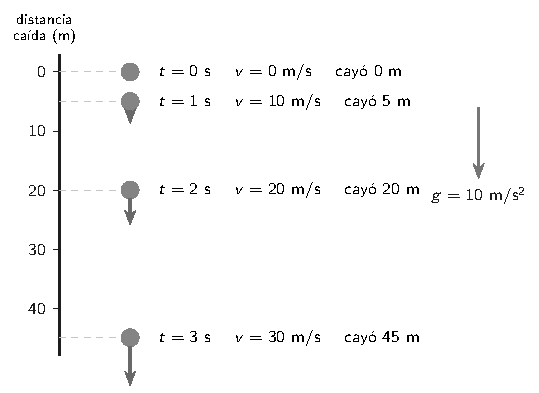
\includegraphics[max width=0.92\linewidth,max height=8.5cm]{fis/mov_caida}
\end{center}
 
\begin{clave}[{Recuerda}] En el punto más alto la velocidad es nula, pero la aceleración no: sigue siendo 10 m/s² hacia abajo. Si la aceleración fuera nula, el cuerpo se quedaría flotando allí.\end{clave}
\subsection{Frenado y distancia de detención}
Cuando un conductor ve un obstáculo, el auto no empieza a frenar de inmediato:

 
\begin{itemize}
  \item \textbf{Tiempo de reacción} (alrededor de 1 s): el auto sigue con la misma velocidad, en MRU.
  \item \textbf{Frenado}: el auto disminuye su velocidad con aceleración constante hasta detenerse, en MRUA.
\end{itemize}
 

\textbf{Ejemplo.} Un auto a 30 m/s, con 1 s de reacción y una aceleración de frenado de 6 m/s²:

 
\begin{itemize}
  \item reacción: $30\cdot 1 = 30$ m;
  \item frenado: de $0 = 30^2 - 2\cdot 6\cdot d$ resulta $d = \dfrac{900}{12} = 75$ m;
  \item distancia total de detención: 105 m.
\end{itemize}
  
\begin{clave}[{La distancia de frenado crece con el cuadrado de la rapidez}] Como $d = \dfrac{v_0^2}{2a}$, con la misma aceleración de frenado, al duplicar la rapidez la distancia de frenado se cuadruplica, y al triplicarla se multiplica por 9. Por eso los límites de velocidad importan tanto.\end{clave}
 
\begin{clave}[{Recuerda}] En un gráfico $v$--$t$ de frenado, la recta baja hasta $v = 0$. La pendiente es la aceleración (negativa si el auto avanzaba en sentido positivo) y el área bajo la recta es la distancia recorrida mientras frena.\end{clave}
\subsection{Lo clave del tema}
\begin{center}\small
\begin{tabularx}{\linewidth}{@{}>{\raggedright\arraybackslash\hsize=0.89\hsize}X>{\raggedright\arraybackslash\hsize=0.68\hsize}X>{\raggedright\arraybackslash\hsize=1.44\hsize}X@{}}
\toprule
 & \textbf{MRU} & \textbf{MRUA} \\
\midrule
Aceleración & $a = 0$ & $a$ constante, distinta de 0 \\
Velocidad & constante & $v = v_0 + a\,t$ \\
Posición & $x = x_0 + v\,t$ & $x = x_0 + v_0\,t + \tfrac{1}{2}\,a\,t^2$ \\
Gráfico $x$--$t$ & recta & parábola \\
Gráfico $v$--$t$ & recta horizontal & recta inclinada: pendiente = $a$ \\
Gráfico $a$--$t$ & sobre el eje & recta horizontal \\
Área bajo $v$--$t$ & \multicolumn{2}{@{}l@{}}{desplazamiento} \\
Caída libre & \multicolumn{2}{@{}l@{}}{MRUA con $g = 10$ m/s² hacia abajo: $v = g\,t$, $h = \tfrac{1}{2}\,g\,t^2$} \\
\bottomrule
\end{tabularx}
\end{center}
 
\begin{clave}[{Recuerda}] · No olvides el $\tfrac{1}{2}$ en $\tfrac{1}{2}\,a\,t^2$.\par · Sin roce del aire, todos los cuerpos caen con la misma aceleración, sin importar su masa.\par · En el punto más alto de un lanzamiento vertical, $v = 0$ pero $a = g$.\par · Con la misma aceleración de frenado, el doble de rapidez implica cuatro veces la distancia de frenado.\end{clave}
 
\begin{clave}[{Método PAES}] 1. Anota los datos con signo: $x_0$, $v_0$, $a$, $t$. 2. Traduce las frases: «parte del reposo» es $v_0 = 0$ y «se detiene» es $v = 0$. 3. Elige la ecuación que tenga solo una incógnita. 4. En gráficos $v$--$t$, usa la pendiente para la aceleración y el área para el desplazamiento.\end{clave}
\begin{elejemplo}{Estilo PAES}
Un conductor que viaja a 20 m/s por una calle recta ve un obstáculo y frena hasta detenerse. El gráfico muestra la velocidad del auto desde el instante en que el conductor ve el obstáculo.

¿Qué distancia recorre el auto desde que el conductor ve el obstáculo hasta que se detiene, y cuál es su aceleración mientras frena?
\begin{center}
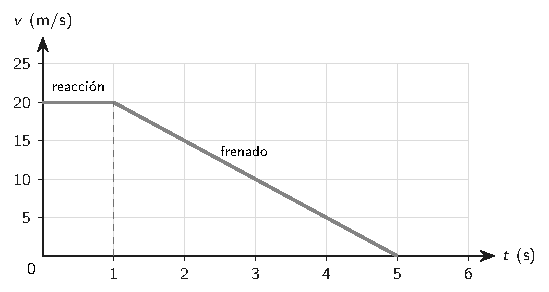
\includegraphics[max width=0.92\linewidth,max height=8.5cm]{fis/mov_frenado}
\end{center}
\alts{60 m y \ensuremath{-}5 m/s²}{40 m y \ensuremath{-}5 m/s²}{100 m y \ensuremath{-}4 m/s²}{60 m y \ensuremath{-}4 m/s²}
\solucion{\textbf{Paso 1. ¿Qué nos piden?} La distancia total (área bajo el gráfico) y la aceleración del frenado (pendiente del segundo tramo).

\textbf{Paso 2. Tramo de reacción.} De 0 a 1 s, velocidad constante de 20 m/s: área $= 20\cdot 1 = 20$ m.

\textbf{Paso 3. Tramo de frenado.} De 1 a 5 s, un triángulo: área $= \dfrac{4\cdot 20}{2} = 40$ m.

\textbf{Paso 4. Distancia total.} $20 + 40 = 60$ m.

\textbf{Paso 5. Aceleración del frenado.} $a = \dfrac{\Delta v}{\Delta t} = \dfrac{0 - 20}{5 - 1} = -5$ m/s². El signo negativo indica que la aceleración es contraria a la velocidad.

\textbf{Respuesta:} 60 m y \ensuremath{-}5 m/s².

\textbf{¿Por qué no las otras?} 40 m cuenta solo el frenado y olvida el tramo de reacción. 100 m multiplica 20 m/s por 5 s, como si el auto nunca hubiera frenado. \ensuremath{-}4 m/s² divide el cambio de velocidad por los 5 s totales, pero el frenado dura 4 s.

\textbf{\color{cienciaD}Para recordar.} En v--t: área = distancia recorrida; pendiente = aceleración.}{A}
\end{elejemplo}

%% =====================================================================
%% fis_newton
\section[Leyes de Newton]{Leyes de Newton}
\modcomun\ \ {\color{gris}\itshape Fuerza y fuerza neta, principio de inercia, relación entre fuerza neta, masa y aceleración, y pares de acción y reacción. Cuerpos con velocidad constante o con aceleración constante, y cómo dibujar e interpretar un diagrama de cuerpo libre.\par}
\subsection{Fuerza y fuerza neta}
Una \textbf{fuerza} es una \textbf{interacción} entre dos cuerpos: uno empuja, tira o atrae al otro. Una fuerza puede cambiar el estado de movimiento de un cuerpo (ponerlo en marcha, frenarlo, desviarlo) o deformarlo.

 

La fuerza es una magnitud \textbf{vectorial}: tiene magnitud, dirección y sentido. Se mide en \textbf{newton} (N) con un \textbf{dinamómetro}: $1\ \text{N} = 1\ \text{kg}\cdot\text{m/s}^2$.

 

Sobre un cuerpo suelen actuar varias fuerzas a la vez. La \textbf{fuerza neta} (o resultante) es su suma vectorial:

 
\begin{itemize}
  \item \textbf{Misma dirección y sentido:} se suman. 30 N y 10 N hacia la derecha dan 40 N hacia la derecha.
  \item \textbf{Misma dirección y sentido contrario:} se restan, y la neta apunta hacia la mayor. 30 N a la derecha y 10 N a la izquierda dan 20 N a la derecha.
  \item \textbf{Fuerzas perpendiculares:} se analizan por separado en cada eje (horizontal y vertical).
\end{itemize}
  
\begin{clave}[{Las fuerzas de esta unidad}] · \textbf{Peso:} la Tierra atrae al cuerpo.\par · \textbf{Normal:} una superficie empuja al cuerpo que se apoya en ella.\par · \textbf{Tensión:} una cuerda tira del cuerpo.\par · \textbf{Fuerza elástica:} un resorte deformado empuja o tira.\par · \textbf{Roce:} una superficie, o el aire, se opone al deslizamiento.\end{clave}
 
\begin{clave}[{Recuerda}] Toda fuerza la ejerce \textbf{un cuerpo sobre otro}. Si no puedes decir qué cuerpo la ejerce, esa fuerza no existe. No hay una «fuerza del movimiento» ni una «fuerza de la inercia».\end{clave}
\subsection{Primera ley: el principio de inercia}
\textbf{Primera ley de Newton.} Si la fuerza neta sobre un cuerpo es cero, el cuerpo mantiene su estado de movimiento: si estaba en reposo, sigue en reposo; si se movía, sigue con \textbf{velocidad constante}, es decir, en línea recta y con la misma rapidez.

 

La \textbf{inercia} es la tendencia de los cuerpos a mantener su velocidad. La \textbf{masa} mide cuánta inercia tiene un cuerpo: cuesta más cambiar la velocidad de un camión que la de una bicicleta.

 

\textbf{Ejemplos.} Cuando un bus frena de golpe, los pasajeros se van hacia adelante: nada los empuja, simplemente siguen moviéndose mientras el bus se detiene. Una sonda en el espacio, lejos de todo planeta, sigue avanzando con los motores apagados.

 
\begin{center}\small
\begin{tabular}{@{}ll@{}}
\toprule
\textbf{Estado del cuerpo} & \textbf{Fuerza neta} \\
\midrule
Reposo & cero \\
Velocidad constante (MRU) & cero \\
La velocidad cambia (rapidez o dirección) & distinta de cero \\
\bottomrule
\end{tabular}
\end{center}
  
\begin{clave}[{Velocidad constante no significa «sin fuerzas»}] Un auto que avanza a 90 km/h constantes por una carretera recta tiene varias fuerzas encima: la que lo impulsa (el roce del camino sobre las ruedas motrices), el roce con el aire, el peso y la normal. Lo que ocurre es que se \textbf{equilibran}: la fuerza neta es cero.\end{clave}
 
\begin{clave}[{Recuerda}] Para mantener un cuerpo en movimiento no se necesita una fuerza neta. En la vida diaria parece que sí, porque el roce frena todo: si empujas un carro y lo sueltas, se detiene por el roce, no porque «se le acabe la fuerza».\end{clave}
\subsection{Segunda ley: fuerza neta, masa y aceleración}
\textbf{Segunda ley de Newton.} La fuerza neta sobre un cuerpo es igual al producto de su masa por su aceleración:

 \[ \vec F_{\text{neta}} = m\,\vec a \] 

La aceleración tiene la \textbf{misma dirección y sentido que la fuerza neta}, no necesariamente que la velocidad. Si la fuerza neta apunta en contra del movimiento, el cuerpo frena.

 
\begin{itemize}
  \item Con la misma masa, el doble de fuerza neta produce el doble de aceleración (proporcionalidad directa).
  \item Con la misma fuerza neta, el doble de masa produce la mitad de aceleración (proporcionalidad inversa).
  \item Fuerza neta constante produce aceleración constante (MRUA).
\end{itemize}
 
\begin{ejemplo}[{Ejemplo resuelto}] Sobre un carro de 4 kg, en un piso sin roce, actúan 30 N hacia la derecha y 10 N hacia la izquierda.\par \textbf{Paso 1.} $F_{\text{neta}} = 30 - 10 = 20$ N hacia la derecha.\par \textbf{Paso 2.} $a = \dfrac{F_{\text{neta}}}{m} = \dfrac{20}{4} = 5\ \text{m/s}^2$ hacia la derecha.\end{ejemplo}
  
\begin{center}
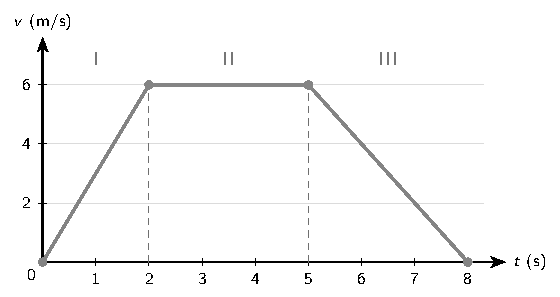
\includegraphics[max width=0.92\linewidth,max height=8.5cm]{fis/fza_vt_newton}
\end{center}
 
\begin{clave}[{Leer la fuerza neta en un gráfico v--t}] La pendiente del gráfico es la aceleración. En el tramo I la rapidez aumenta: la fuerza neta apunta en el sentido del movimiento. En el tramo II la rapidez es constante: la fuerza neta es cero. En el tramo III la rapidez disminuye: la fuerza neta apunta en contra del movimiento.\end{clave}
\subsection{Tercera ley: acción y reacción}
\textbf{Tercera ley de Newton.} Si un cuerpo A ejerce una fuerza sobre un cuerpo B, entonces B ejerce sobre A una fuerza de \textbf{igual magnitud}, \textbf{igual dirección} y \textbf{sentido contrario}. Las fuerzas siempre aparecen de a pares.

 

Características de un par de acción y reacción:

 
\begin{itemize}
  \item Actúan sobre \textbf{cuerpos distintos}; por eso \textbf{nunca se anulan} entre sí.
  \item Son del mismo tipo: ambas de contacto, o ambas gravitacionales.
  \item Aparecen y desaparecen al mismo tiempo.
\end{itemize}
 

\textbf{Ejemplos.} Al caminar empujas el suelo hacia atrás, y el suelo te empuja hacia adelante. Un cohete empuja los gases hacia abajo, y los gases empujan al cohete hacia arriba. Si un camión choca con un auto, ambos reciben fuerzas de igual magnitud; el auto, de menor masa, sufre una aceleración mucho mayor.

  
\begin{center}
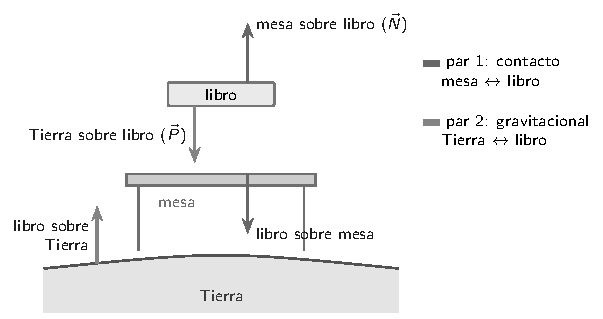
\includegraphics[max width=0.92\linewidth,max height=8.5cm]{fis/fza_pares}
\end{center}
 
\begin{clave}[{Recuerda}] El peso y la normal de un libro sobre una mesa tienen igual magnitud y sentido contrario, pero \textbf{no} son un par de acción y reacción: las dos actúan sobre el libro y son de distinto tipo. La reacción del peso es la fuerza con que el libro atrae a la Tierra; la reacción de la normal es la fuerza con que el libro empuja a la mesa.\end{clave}
\subsection{Diagrama de cuerpo libre}
Un \textbf{diagrama de cuerpo libre} (DCL) muestra todas las fuerzas que actúan sobre \textbf{un solo cuerpo}. Para construirlo:

 
\begin{enumerate}
  \item Elige el cuerpo y sepáralo mentalmente de todo lo que lo rodea.
  \item Represéntalo como un punto.
  \item Dibuja el \textbf{peso}, siempre vertical hacia abajo.
  \item Revisa qué toca al cuerpo: cada contacto puede aportar una fuerza (normal y roce de una superficie, tensión de una cuerda, empuje de una mano).
  \item Dibuja cada flecha con un largo proporcional a su magnitud.
\end{enumerate}
 

Después aplica Newton \textbf{por ejes}. Si el bloque de la figura se mueve con velocidad constante, en el eje vertical $N = P$ y en el horizontal $F = f_r$. Si $F > f_r$, acelera hacia la derecha.

  
\begin{center}
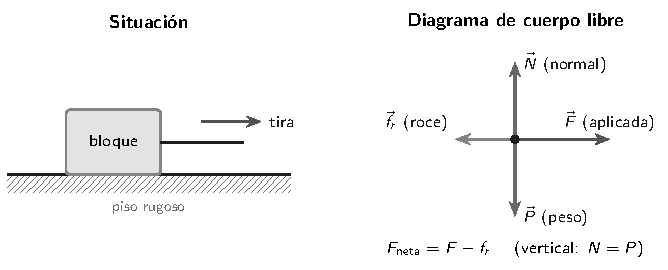
\includegraphics[max width=0.92\linewidth,max height=8.5cm]{fis/fza_dcl_bloque}
\end{center}
 
\begin{clave}[{Recuerda}] En el DCL van solo las fuerzas que \textbf{otros cuerpos ejercen sobre el cuerpo elegido}. No dibujes las fuerzas que el cuerpo ejerce sobre otros, ni $m\vec a$ como si fuera una fuerza más.\end{clave}
\subsection{Lo clave del tema}
\begin{center}\small
\begin{tabularx}{\linewidth}{@{}>{\raggedright\arraybackslash\hsize=0.76\hsize}X>{\raggedright\arraybackslash\hsize=1.12\hsize}X>{\raggedright\arraybackslash\hsize=1.12\hsize}X@{}}
\toprule
\textbf{Ley} & \textbf{Enunciado} & \textbf{Cómo se usa en la PAES} \\
\midrule
Primera (inercia) & fuerza neta cero: reposo o velocidad constante & velocidad constante indica fuerzas equilibradas \\
Segunda & $\vec F_{\text{neta}} = m\,\vec a$ & calcular la aceleración o la fuerza; la aceleración apunta como la fuerza neta \\
Tercera (acción y reacción) & fuerzas de igual magnitud y sentido contrario, sobre cuerpos distintos & choques, caminar, cohetes; los pares no se anulan \\
Diagrama de cuerpo libre & solo las fuerzas que actúan sobre el cuerpo & sumar las fuerzas por ejes \\
\bottomrule
\end{tabularx}
\end{center}
 
\begin{clave}[{Recuerda}] · Velocidad constante no significa ausencia de fuerzas: significa fuerza neta cero.\par · La aceleración, no la velocidad, tiene el sentido de la fuerza neta.\par · El peso y la normal no son un par de acción y reacción.\par · En un gráfico v--t, la pendiente es la aceleración; por la masa da la fuerza neta.\end{clave}
 
\begin{clave}[{Método PAES}] 1. Elige el cuerpo y haz su DCL. 2. Decide si su velocidad es constante o cambia. 3. Si es constante, iguala las fuerzas en cada eje; si cambia, usa $F_{\text{neta}} = m\,a$. 4. En preguntas de acción y reacción, revisa sobre qué cuerpo actúa cada fuerza. 5. Descarta las alternativas que inventan fuerzas sin un cuerpo que las ejerza.\end{clave}
\begin{elejemplo}{Estilo PAES}
Un carro de 2 kg se mueve en línea recta sobre una superficie horizontal. El gráfico muestra su rapidez en función del tiempo.

¿Cuál de las siguientes afirmaciones sobre la fuerza neta que actúa sobre el carro es correcta?
\begin{center}
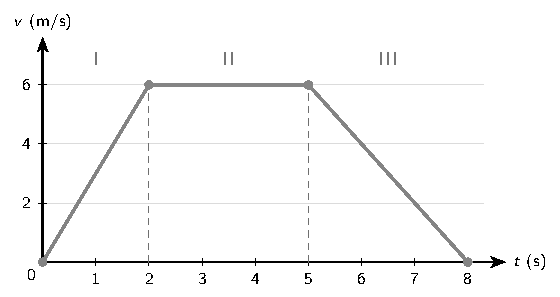
\includegraphics[max width=0.92\linewidth,max height=8.5cm]{fis/fza_vt_newton}
\end{center}
\altslargas{Entre 0 s y 2 s la fuerza neta es de 12 N, y entre 2 s y 5 s es nula.}{Entre 0 s y 2 s la fuerza neta es de 6 N, y entre 2 s y 5 s es nula.}{Entre 2 s y 5 s no actúa ninguna fuerza sobre el carro.}{Entre 5 s y 8 s la fuerza neta tiene el mismo sentido que el movimiento.}
\solucion{\textbf{Paso 1. ¿Qué nos piden?} La fuerza neta sobre el carro en cada tramo, a partir de un gráfico de rapidez en función del tiempo.

\textbf{Paso 2. Calcula la aceleración de cada tramo.} La aceleración es la pendiente del gráfico. Entre 0 y 2 s: $a = \dfrac{6 - 0}{2 - 0} = 3\ \text{m/s}^2$. Entre 2 y 5 s la rapidez no cambia: $a = 0$. Entre 5 y 8 s: $a = \dfrac{0 - 6}{8 - 5} = -2\ \text{m/s}^2$.

\textbf{Paso 3. Aplica la segunda ley.} $F_{\text{neta}} = m\,a$. Entre 0 y 2 s: $2\cdot 3 = 6$ N. Entre 2 y 5 s: $2\cdot 0 = 0$. Entre 5 y 8 s: $2\cdot 2 = 4$ N, en contra del movimiento.

\textbf{Respuesta:} entre 0 s y 2 s la fuerza neta es de 6 N, y entre 2 s y 5 s es nula.

\textbf{¿Por qué no las otras?} 12 N sale de multiplicar la masa por la rapidez (2 · 6), y la segunda ley usa la aceleración. Que la fuerza neta sea nula no significa que no haya fuerzas: sobre el carro actúan al menos el peso y la normal, que se equilibran. Entre 5 y 8 s el carro frena, así que la aceleración, y con ella la fuerza neta, apunta en contra del movimiento.

\textbf{\color{cienciaD}Para recordar.} La pendiente del gráfico v--t es la aceleración; multiplicada por la masa da la fuerza neta.}{B}
\end{elejemplo}

%% =====================================================================
%% fis_fuerzas
\section[Peso, normal, tensión y fuerza elástica]{Peso, normal, tensión y fuerza elástica}
\modcomun\ \ {\color{gris}\itshape Las fuerzas más comunes: peso (masa frente a peso, otros planetas), normal, tensión en cuerdas y poleas, y fuerza elástica con la ley de Hooke y sus gráficos. Problemas con diagrama de cuerpo libre en superficies horizontales.\par}
\subsection{Masa y peso}
La \textbf{masa} ($m$) mide la cantidad de materia de un cuerpo y su inercia. Se mide en kilogramos (kg) con una \textbf{balanza}, y es la misma en cualquier lugar del universo.

 

El \textbf{peso} ($\vec P$) es la fuerza con que un planeta, u otro astro, atrae a un cuerpo. Es vertical, apunta hacia el centro del planeta y se mide en newton (N) con un \textbf{dinamómetro}:

 \[ P = m\,g \] 

donde $g$ es la aceleración de gravedad del lugar: cerca de $10\ \text{m/s}^2$ en la Tierra, $1{,}6\ \text{m/s}^2$ en la Luna y $3{,}7\ \text{m/s}^2$ en Marte.

  
\begin{center}\small
\begin{tabular}{@{}llll@{}}
\toprule
\textbf{Lugar} & \textbf{$g$ (m/s²)} & \textbf{Masa} & \textbf{Peso} \\
\midrule
Tierra & 10 & 60 kg & 600 N \\
Marte & 3,7 & 60 kg & 222 N \\
Luna & 1,6 & 60 kg & 96 N \\
\bottomrule
\end{tabular}
\end{center}
 
\begin{clave}[{Recuerda}] En la vida diaria decimos «peso 60 kilos», pero en física esa cantidad es la masa. Tu peso en la Tierra es de unos 600 N. Si viajas a la Luna, tu masa no cambia; tu peso se reduce a cerca de la sexta parte.\end{clave}
\subsection{Fuerza normal}
La \textbf{normal} ($\vec N$) es la fuerza que ejerce una superficie sobre un cuerpo apoyado en ella. Es \textbf{perpendicular} a la superficie y empuja hacia afuera de ella. Solo existe si hay contacto.

 

La normal se ajusta a cada situación: \textbf{no siempre es igual al peso}. Para encontrarla, haz el DCL y aplica Newton en la dirección perpendicular a la superficie.

 
\begin{center}\small
\begin{tabular}{@{}ll@{}}
\toprule
\textbf{Cuerpo en reposo sobre un piso horizontal} & \textbf{Normal} \\
\midrule
solo actúan el peso y la normal & $N = P$ \\
lo empujas hacia abajo con una fuerza $F$ & $N = P + F$ \\
tiras de él hacia arriba con $F$, sin levantarlo & $N = P - F$ \\
tiene encima otro cuerpo de peso $P_2$ & $N = P + P_2$ \\
\bottomrule
\end{tabular}
\end{center}
 

En un plano inclinado, la normal es menor que el peso.

  
\begin{ejemplo}[{Ejemplo resuelto}] Una caja de 5 kg está en el piso y tiras de ella hacia arriba con 20 N, sin levantarla.\par \textbf{Paso 1.} $P = 5\cdot 10 = 50$ N hacia abajo.\par \textbf{Paso 2.} Hacia arriba actúan tu fuerza y la normal. En reposo: $N + 20 = 50$.\par \textbf{Paso 3.} $N = 30$ N.\end{ejemplo}
 
\begin{clave}[{Recuerda}] El peso y la normal no son un par de acción y reacción: actúan sobre el mismo cuerpo. La reacción de la normal es la fuerza con que el cuerpo empuja a la superficie.\end{clave}
\subsection{Tensión y poleas}
La \textbf{tensión} ($\vec T$) es la fuerza que ejerce una cuerda tensa sobre el cuerpo atado a ella. Siempre \textbf{tira} del cuerpo, a lo largo de la cuerda.

 

En la PAES las cuerdas suelen ser \textbf{ideales}: inextensibles y de masa despreciable. Una cuerda ideal transmite la \textbf{misma tensión} en todos sus puntos.

 

Una \textbf{polea ideal}, sin masa ni roce, solo cambia la dirección de la cuerda: la tensión es la misma a ambos lados.

 

\textbf{Cuerpo que cuelga en reposo o con velocidad constante:} $T = P = m\,g$.

 
\begin{clave}[{Recuerda}] Si la cuerda es gruesa y pesada (no ideal), la tensión es mayor arriba que abajo: la parte superior sostiene, además del cuerpo, el peso de la cuerda que cuelga bajo ella.\end{clave}
  
\begin{center}
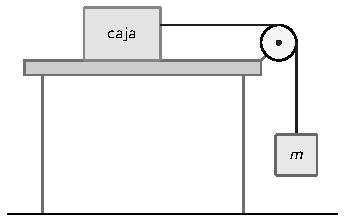
\includegraphics[max width=0.92\linewidth,max height=8.5cm]{fis/fza_polea}
\end{center}
 
\begin{ejemplo}[{Ejemplo resuelto}] En la figura, la caja está en reposo y cuelga un cuerpo de 1,5 kg.\par \textbf{Paso 1.} El cuerpo colgante está en reposo: $T = m\,g = 1{,}5\cdot 10 = 15$ N.\par \textbf{Paso 2.} La cuerda ideal tira de la caja, en horizontal, con los mismos 15 N.\par \textbf{Paso 3.} La caja no se mueve: el roce estático de la mesa sobre ella también vale 15 N.\end{ejemplo}
\subsection{Fuerza elástica: ley de Hooke}
Un resorte estirado o comprimido ejerce una \textbf{fuerza elástica} que tiende a devolverlo a su longitud natural. La \textbf{ley de Hooke} dice que la magnitud de esa fuerza es proporcional a la \textbf{deformación}:

 \[ F = k\,\Delta x \] 
\begin{itemize}
  \item $\Delta x = L - L_0$: cuánto cambió la longitud respecto de la longitud natural $L_0$. No es la longitud total.
  \item $k$: constante elástica, en N/m o N/cm. Un $k$ mayor indica un resorte más rígido, que cuesta más deformar.
  \item El gráfico de $F$ en función de $\Delta x$ es una recta que pasa por el origen, y su \textbf{pendiente es $k$}.
  \item La ley vale hasta el \textbf{límite elástico}. Más allá, el resorte queda deformado y el gráfico deja de ser una recta.
\end{itemize}
 
\begin{ejemplo}[{Ejemplo resuelto}] Con 30 N un resorte se estira 20 cm. ¿Qué fuerza lo estira 45 cm?\par \textbf{Paso 1.} $k = \dfrac{30}{20} = 1{,}5$ N/cm.\par \textbf{Paso 2.} $F = 1{,}5\cdot 45 = 67{,}5$ N.\end{ejemplo}
  
\begin{center}
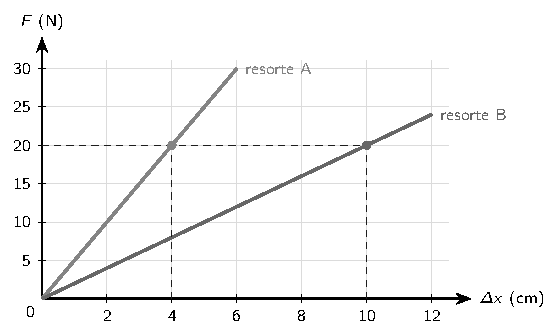
\includegraphics[max width=0.92\linewidth,max height=8.5cm]{fis/fza_hooke_grafico}
\end{center}
 
\begin{clave}[{Leer el gráfico}] Con 20 N, el resorte A se deforma 4 cm y el B, 10 cm. Entonces $k_A = \dfrac{20}{4} = 5$ N/cm y $k_B = \dfrac{20}{10} = 2$ N/cm. El resorte A es más rígido: su recta es más empinada.\end{clave}
\subsection{Lo clave del tema}
\begin{center}\small
\begin{tabularx}{\linewidth}{@{}>{\raggedright\arraybackslash\hsize=0.42\hsize}X>{\raggedright\arraybackslash\hsize=0.84\hsize}X>{\raggedright\arraybackslash\hsize=1.22\hsize}X>{\raggedright\arraybackslash\hsize=1.52\hsize}X@{}}
\toprule
\textbf{Fuerza} & \textbf{Quién la ejerce} & \textbf{Dirección} & \textbf{Cómo se calcula} \\
\midrule
Peso & el planeta & vertical, hacia abajo & $P = m\,g$ \\
Normal & la superficie de apoyo & perpendicular a la superficie & con el DCL; no siempre es igual al peso \\
Tensión & una cuerda & a lo largo de la cuerda, tirando & con el DCL; igual en toda una cuerda ideal \\
Elástica & un resorte & hacia la longitud natural & $F = k\,\Delta x$ \\
\bottomrule
\end{tabularx}
\end{center}
 
\begin{clave}[{Recuerda}] · La masa no cambia de un planeta a otro; el peso sí.\par · En la ley de Hooke se usa la deformación $\Delta x$, no la longitud total.\par · La pendiente del gráfico $F$--$\Delta x$ es la constante $k$.\end{clave}
 
\begin{clave}[{Método PAES}] 1. Haz el DCL del cuerpo. 2. Calcula el peso con $P = m\,g$. 3. Decide si la aceleración es cero o no, y hacia dónde apunta. 4. Plantea la suma de fuerzas en el eje que corresponda. 5. En resortes, convierte longitudes en deformaciones antes de usar $F = k\,\Delta x$.\end{clave}
\begin{elejemplo}{Estilo PAES}
El gráfico muestra la fuerza aplicada en función de la deformación para dos resortes, A y B.

¿Cuál de las siguientes afirmaciones es correcta?
\begin{center}
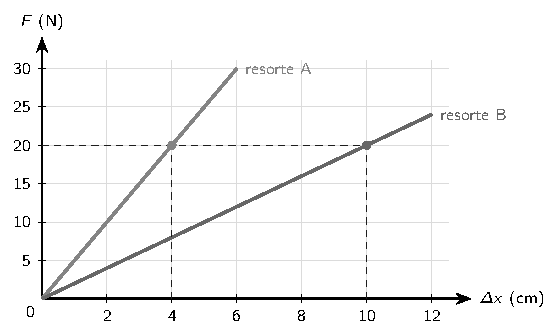
\includegraphics[max width=0.92\linewidth,max height=8.5cm]{fis/fza_hooke_grafico}
\end{center}
\altslargas{El resorte B es más rígido, porque se estira más con la misma fuerza.}{Ambos resortes tienen la misma constante, porque sus gráficos son rectas que pasan por el origen.}{La constante del resorte A es 0,2 N/cm.}{El resorte A es más rígido: su constante es 5 N/cm y la de B es 2 N/cm.}
\solucion{\textbf{Paso 1. ¿Qué nos piden?} Comparar las constantes elásticas a partir del gráfico.

\textbf{Paso 2. Lee un punto de cada recta.} Con 20 N, A se deforma 4 cm y B se deforma 10 cm.

\textbf{Paso 3. Calcula las pendientes.} $k_A = \dfrac{20}{4} = 5$ N/cm y $k_B = \dfrac{20}{10} = 2$ N/cm. A necesita más fuerza por cada centímetro: es más rígido.

\textbf{Respuesta:} A es más rígido: su constante es 5 N/cm y la de B es 2 N/cm.

\textbf{¿Por qué no las otras?} Estirarse más con la misma fuerza indica un resorte más blando, no más rígido. Que ambos gráficos sean rectas por el origen indica que ambos cumplen la ley de Hooke, pero sus pendientes son distintas. 0,2 sale de dividir la deformación por la fuerza ($\dfrac{4}{20}$), al revés.

\textbf{\color{cienciaD}Para recordar.} En el gráfico F--\ensuremath{\Delta}x, la recta más empinada es la del resorte más rígido.}{D}
\end{elejemplo}

%% =====================================================================
%% fis_roce
\section[Fuerza de roce]{Fuerza de roce}
\modcomun\ \ {\color{gris}\itshape Roce estático (hasta su valor máximo \ensuremath{\mu}s N) y roce cinético (\ensuremath{\mu}k N), su dependencia de las superficies y de la normal, y la lectura de gráficos de roce en función de la fuerza aplicada. Roce con el aire en términos cualitativos: velocidad límite y paracaídas.\par}
\subsection{Qué es la fuerza de roce}
La \textbf{fuerza de roce} ($\vec f_r$) aparece cuando dos superficies en contacto deslizan, o tienden a deslizar, una sobre otra. Es \textbf{paralela} a las superficies y se \textbf{opone al deslizamiento}, o a la tendencia a deslizar.

 

Se origina en las irregularidades microscópicas de las superficies, que se traban y se adhieren entre sí. Incluso una superficie que parece lisa es rugosa vista al microscopio.

 

Su magnitud depende de:

 
\begin{itemize}
  \item el \textbf{tipo de superficies} en contacto (madera sobre cemento, goma sobre asfalto, acero sobre hielo), que se resume en un \textbf{coeficiente de roce} $\mu$, sin unidad;
  \item la \textbf{fuerza normal}: mientras más se aprietan las superficies, mayor es el roce.
\end{itemize}
 

En el modelo que usa la PAES, el roce entre sólidos \textbf{no depende del área de contacto} ni de la rapidez del deslizamiento.

  
\begin{clave}[{Útil y perjudicial}] Sin roce no podrías caminar, los autos no podrían frenar ni doblar y los clavos se soltarían. Pero el roce también desgasta piezas y transforma energía en calor: por eso se usan lubricantes y rodamientos en las máquinas.\end{clave}
 
\begin{clave}[{Recuerda}] El roce se opone al deslizamiento entre las superficies, no siempre al movimiento del cuerpo. Cuando caminas, tu pie empuja el suelo hacia atrás, y el roce del suelo sobre tu zapato apunta hacia adelante: es la fuerza que te impulsa.\end{clave}
\subsection{Roce estático}
Mientras el cuerpo está \textbf{en reposo} respecto de la superficie, actúa el \textbf{roce estático}. Su magnitud no es fija: toma el valor justo para impedir el deslizamiento, igual a la fuerza que tiende a mover el cuerpo.

 

Pero tiene un tope. El roce estático máximo es:

 \[ f_{s,\text{máx}} = \mu_s\,N \] 

donde $\mu_s$ es el coeficiente de roce estático. Si la fuerza aplicada supera ese valor, el cuerpo empieza a deslizar.

 
\begin{clave}[{Recuerda}] El producto $\mu_s\,N$ es el roce estático \textbf{máximo}, no el roce que actúa siempre. Úsalo solo cuando el cuerpo está a punto de deslizar.\end{clave}
  
\begin{ejemplo}[{Ejemplo resuelto}] Un bloque de 2 kg está sobre un piso horizontal, con $\mu_s = 0{,}6$.\par \textbf{Paso 1.} Normal: $N = P = 2\cdot 10 = 20$ N.\par \textbf{Paso 2.} Roce estático máximo: $f_{s,\text{máx}} = 0{,}6\cdot 20 = 12$ N.\par \textbf{Paso 3.} Si lo empujas con 5 N, no se mueve y el roce vale 5 N. Con 10 N, no se mueve y el roce vale 10 N. Con 13 N, se supera el máximo y el bloque empieza a moverse.\end{ejemplo}
 
\begin{center}\small
\begin{tabular}{@{}lll@{}}
\toprule
\textbf{Fuerza aplicada} & \textbf{¿Se mueve?} & \textbf{Roce} \\
\midrule
5 N & no & 5 N (estático) \\
10 N & no & 10 N (estático) \\
12 N & a punto de moverse & 12 N (estático máximo) \\
\bottomrule
\end{tabular}
\end{center}
\subsection{Roce cinético}
Cuando el cuerpo ya \textbf{desliza}, actúa el \textbf{roce cinético}, de magnitud prácticamente constante:

 \[ f_k = \mu_k\,N \] 

Para un mismo par de superficies, $\mu_k < \mu_s$: cuesta más poner un cuerpo en movimiento que mantenerlo deslizando. Por eso, al empujar un mueble, hace falta un empujón fuerte para que parta, y después basta una fuerza menor.

 
\begin{itemize}
  \item Si la fuerza aplicada es igual a $f_k$, la fuerza neta es cero y el cuerpo desliza con \textbf{velocidad constante}.
  \item Si es mayor, el cuerpo acelera: $a = \dfrac{F - f_k}{m}$.
  \item Si deja de aplicarse, el roce lo frena hasta detenerlo, con una aceleración $\dfrac{f_k}{m}$ opuesta al movimiento.
\end{itemize}
  
\begin{ejemplo}[{Ejemplo resuelto}] El mismo bloque de 2 kg, ahora con $\mu_k = 0{,}4$, desliza por el piso.\par \textbf{Paso 1.} $f_k = 0{,}4\cdot 20 = 8$ N.\par \textbf{Paso 2.} Empujado con 12 N: $a = \dfrac{12 - 8}{2} = 2\ \text{m/s}^2$.\par \textbf{Paso 3.} Empujado con 8 N: la fuerza neta es cero y avanza con velocidad constante.\par \textbf{Paso 4.} Si lo sueltas: frena con $a = \dfrac{8}{2} = 4\ \text{m/s}^2$.\end{ejemplo}
 
\begin{clave}[{Recuerda}] El roce cinético no aumenta si empujas más fuerte: depende solo de $\mu_k$ y de la normal. Empujar más fuerte aumenta la aceleración.\end{clave}
\subsection{Gráficos del roce}
\begin{center}
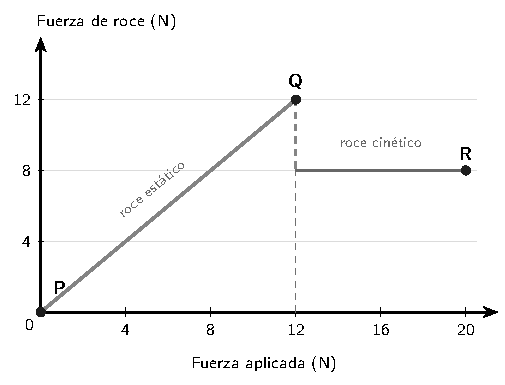
\includegraphics[max width=0.92\linewidth,max height=8.5cm]{fis/fza_roce_grafico}
\end{center}
  

Al aumentar poco a poco la fuerza horizontal aplicada a un bloque en reposo:

 
\begin{itemize}
  \item \textbf{Tramo P--Q:} el bloque sigue en reposo. El roce estático crece junto con la fuerza aplicada y la iguala en todo momento.
  \item \textbf{Punto Q:} se alcanza el roce estático máximo, 12 N, y el bloque empieza a deslizar.
  \item \textbf{Tramo Q--R:} el bloque desliza. El roce es cinético y constante, 8 N, menor que el máximo estático, aunque la fuerza aplicada siga creciendo.
\end{itemize}
 
\begin{clave}[{Recuerda}] En el tramo Q--R el bloque acelera cada vez más, porque la fuerza aplicada crece y el roce se mantiene. Con una fuerza aplicada de 20 N, la fuerza neta es $20 - 8 = 12$ N.\end{clave}
 
\begin{clave}[{Gráficos de fuerza en función del tiempo}] Si el bloque desliza con velocidad constante durante un tramo, en ese tramo la fuerza aplicada es igual al roce cinético. El valor de la fuerza justo cuando el bloque empieza a moverse es el roce estático máximo.\end{clave}
\subsection{Roce con el aire}
Un cuerpo que se mueve en el aire, o en el agua, recibe una fuerza de roce opuesta a su movimiento. A diferencia del roce entre sólidos, este roce \textbf{aumenta con la rapidez}. También aumenta con el \textbf{área} que el cuerpo presenta de frente al avance, y depende de su \textbf{forma}: las formas aerodinámicas lo reducen.

 

\textbf{Caída de un paracaidista} (figura):

 
\begin{itemize}
  \item \textbf{I:} al saltar, el roce es pequeño y la rapidez aumenta. A medida que cae más rápido, el roce crece y la aceleración disminuye.
  \item \textbf{II:} el roce iguala al peso. La fuerza neta es cero y cae con una \textbf{velocidad límite} constante, $v_1$.
  \item \textbf{III:} al abrir el paracaídas, el área aumenta mucho y el roce supera al peso. La fuerza neta apunta hacia arriba y el paracaidista \textbf{frena}.
  \item \textbf{IV:} al frenar, el roce disminuye hasta igualar de nuevo al peso: nueva velocidad límite $v_2$, mucho menor.
\end{itemize}
  
\begin{center}
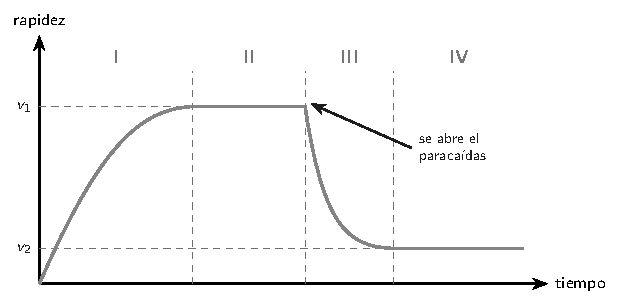
\includegraphics[max width=0.92\linewidth,max height=8.5cm]{fis/fza_paracaidas}
\end{center}
 
\begin{clave}[{Recuerda}] En el vacío, todos los cuerpos caen con la misma aceleración $g$, sin importar su masa. En el aire, una hoja de papel extendida cae más lento que una hoja igual arrugada: tienen la misma masa, pero distinta área frente al aire.\end{clave}
\subsection{Lo clave del tema}
\begin{center}\small
\begin{tabularx}{\linewidth}{@{}>{\raggedright\arraybackslash\hsize=0.37\hsize}X>{\raggedright\arraybackslash\hsize=1.17\hsize}X>{\raggedright\arraybackslash\hsize=1.23\hsize}X>{\raggedright\arraybackslash\hsize=1.23\hsize}X@{}}
\toprule
\textbf{Tipo de roce} & \textbf{Cuándo actúa} & \textbf{Magnitud} & \textbf{Depende de} \\
\midrule
Estático & cuerpo en reposo que tiende a deslizar & igual a la fuerza que tiende a moverlo, hasta $\mu_s\,N$ & superficies y normal \\
Cinético & cuerpo que desliza & $\mu_k\,N$, constante & superficies y normal; no del área ni de la rapidez \\
Con el aire & cuerpo que se mueve en un fluido & crece con la rapidez & rapidez, área y forma \\
\bottomrule
\end{tabularx}
\end{center}
 
\begin{clave}[{Recuerda}] · $\mu_k < \mu_s$: cuesta más hacer partir un cuerpo que mantenerlo deslizando.\par · El roce estático no siempre vale $\mu_s\,N$: ese es su máximo.\par · Con roce y velocidad constante, la fuerza aplicada iguala al roce cinético.\par · Velocidad límite: el roce del aire iguala al peso.\end{clave}
 
\begin{clave}[{Método PAES}] 1. Decide si el cuerpo está en reposo o desliza. 2. Calcula la normal con el DCL. 3. En reposo, el roce iguala a la fuerza que tiende a moverlo (sin pasar de $\mu_s\,N$); deslizando, vale $\mu_k\,N$. 4. Aplica $F_{\text{neta}} = m\,a$. 5. En gráficos, busca dónde empieza el movimiento y dónde la velocidad es constante.\end{clave}
\begin{elejemplo}{PAES Invierno 2026, adaptada}
Un bloque de 2 kg está en reposo sobre una superficie horizontal rugosa. Se le aplica una fuerza horizontal cuya magnitud cambia en el tiempo como muestra el gráfico. El bloque comienza a moverse justo a los 4 s, y entre los 6 s y los 8 s se mueve con velocidad constante.

Si $g = 10\ \text{m/s}^2$, ¿cuáles son los coeficientes de roce estático y cinético entre el bloque y la superficie?
\begin{center}
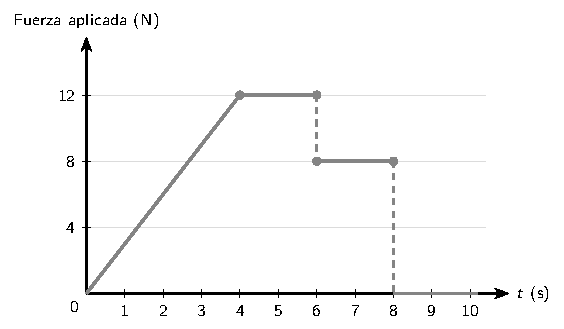
\includegraphics[max width=0.92\linewidth,max height=8.5cm]{fis/fza_fuerza_tiempo}
\end{center}
\alts{$\mu_s = 0{,}4$ y $\mu_k = 0{,}6$}{$\mu_s = 6$ y $\mu_k = 4$}{$\mu_s = 0{,}6$ y $\mu_k = 0{,}4$}{$\mu_s = 0{,}6$ y $\mu_k = 0$}
\solucion{\textbf{Paso 1. ¿Qué nos piden?} Los dos coeficientes de roce, a partir de un gráfico de fuerza aplicada.

\textbf{Paso 2. Calcula la normal.} Superficie horizontal, sin otras fuerzas verticales: $N = P = 2\cdot 10 = 20$ N.

\textbf{Paso 3. Roce estático.} El bloque empieza a moverse a los 4 s, cuando la fuerza vale 12 N: ese es el roce estático máximo. $\mu_s = \dfrac{12}{20} = 0{,}6$.

\textbf{Paso 4. Roce cinético.} Entre 6 s y 8 s el bloque se mueve con velocidad constante: la fuerza neta es cero y el roce cinético iguala a la fuerza aplicada, 8 N. $\mu_k = \dfrac{8}{20} = 0{,}4$.

\textbf{Respuesta:} $\mu_s = 0{,}6$ y $\mu_k = 0{,}4$.

\textbf{¿Por qué no las otras?} Intercambiar los valores daría $\mu_k > \mu_s$, y el roce cinético es menor que el estático máximo. 6 y 4 salen de dividir por la masa en vez de por la normal; los coeficientes no tienen unidad y suelen ser menores que 1. Después de los 8 s la fuerza aplicada es cero, pero el roce sigue actuando hasta que el bloque se detiene: $\mu_k$ no es cero.

\textbf{\color{cienciaD}Para recordar.} Arranque: roce estático máximo. Velocidad constante: roce cinético. Ambos se dividen por la normal.}{C}
\end{elejemplo}

\chapter{Energía y Tierra}
%% =====================================================================
%% fis_deriva
\section[Deriva continental y tectónica de placas]{Deriva continental y tectónica de placas}
\modcomun\ \ {\color{gris}\itshape La deriva continental de Wegener y sus evidencias (encaje de los continentes, fósiles, rocas y paleoclimas), la expansión del fondo oceánico, los límites divergentes, convergentes y transformantes, y sus consecuencias: sismos, volcanismo y relieve, con el caso de Chile.\par}
\subsection{Wegener y la deriva continental}
En 1912, el meteorólogo alemán \textbf{Alfred Wegener} propuso la \textbf{teoría de la deriva continental}: los continentes no han estado siempre en el mismo lugar. Hace unos 300 a 200 millones de años formaban un solo supercontinente, \textbf{Pangea}, rodeado por un único océano, \textbf{Pantalasa}. Pangea se fragmentó y los continentes se fueron desplazando lentamente hasta sus posiciones actuales.

 

Wegener reunió evidencias de áreas muy distintas: geografía, paleontología, geología y climatología. Las verás en la diapositiva siguiente.

 
\begin{clave}[{Por qué no se aceptó al principio}] Wegener no pudo explicar de forma convincente \textbf{qué fuerza} movía los continentes. Pensaba que los continentes «surcaban» el fondo oceánico, y los geólogos de la época mostraron que eso era imposible. La idea fue rechazada durante décadas.\end{clave}
  
\begin{center}
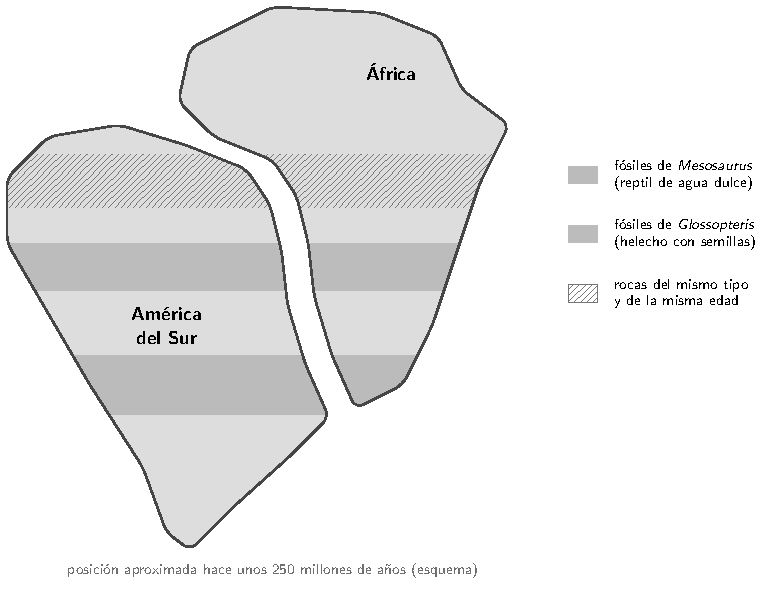
\includegraphics[max width=0.92\linewidth,max height=8.5cm]{fis/tie_wegener}
\end{center}
\subsection{Las evidencias de Wegener}
\textbf{1. Encaje de los continentes.} Las costas de América del Sur y de África calzan como piezas de un rompecabezas, y el ajuste es aún mejor si se usa el borde de la plataforma continental, bajo el mar.

 

\textbf{2. Fósiles.} Se encuentran fósiles de las mismas especies en continentes hoy separados por océanos. \emph{Mesosaurus}, un pequeño reptil de agua dulce, aparece solo en el sur de Brasil y en el sur de África: no pudo cruzar un océano salado. \emph{Glossopteris}, un helecho con semillas pesadas, aparece en América del Sur, África, India, Australia y la Antártica.

  

\textbf{3. Rocas y cordilleras.} Rocas del mismo tipo y la misma edad, y cordilleras con la misma estructura, continúan de un continente a otro: los montes Apalaches de América del Norte continúan en las montañas de Escocia y Escandinavia.

 

\textbf{4. Paleoclimas.} Hay huellas de antiguos glaciares en zonas que hoy son tropicales (India, África, Brasil) y restos de grandes bosques, convertidos en carbón, en la Antártica. Esos continentes estuvieron en otras latitudes.

 
\begin{clave}[{Recuerda}] Ninguna evidencia sola prueba la deriva; la fuerza del argumento está en que \textbf{evidencias independientes} apuntan a la misma conclusión: los continentes estuvieron unidos y se han desplazado.\end{clave}
\subsection{La expansión del fondo oceánico}
En la década de 1960, el estudio del fondo de los océanos dio la pieza que faltaba. \textbf{Harry Hess} propuso la \textbf{expansión del fondo oceánico}:

 
\begin{itemize}
  \item En las \textbf{dorsales oceánicas}, cordilleras submarinas como la dorsal mesoatlántica, sube \textbf{magma} desde el manto, se enfría y forma corteza oceánica nueva.
  \item La corteza nueva empuja a la anterior hacia ambos lados: el océano se ensancha unos pocos centímetros por año.
  \item En las \textbf{fosas oceánicas}, la corteza oceánica antigua se hunde en el manto (subducción). Así la Tierra no crece.
\end{itemize}
 

\textbf{Evidencias:} las rocas son más jóvenes junto a la dorsal y más antiguas a medida que se alejan, en forma simétrica; los sedimentos son más gruesos lejos de la dorsal; y la corteza oceánica más antigua tiene unos 180 millones de años, mucho menos que muchas rocas continentales.

  
\begin{center}
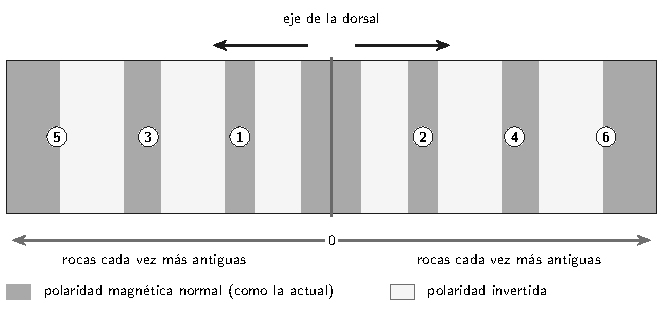
\includegraphics[max width=0.92\linewidth,max height=8.5cm]{fis/tie_dorsal}
\end{center}
 
\begin{clave}[{Bandas magnéticas}] Al solidificarse, algunos minerales de la roca quedan orientados según el campo magnético terrestre de ese momento, que se invierte cada cierto tiempo. Por eso el fondo muestra franjas de polaridad normal e invertida \textbf{simétricas} a ambos lados de la dorsal.\end{clave}
\subsection{Tectónica de placas y tipos de límites}
La \textbf{teoría de la tectónica de placas} une la deriva continental y la expansión del fondo oceánico. La capa externa rígida de la Tierra, la \textbf{litosfera}, está dividida en \textbf{placas} que se desplazan lentamente sobre la \textbf{astenosfera}, una capa plástica del manto. Los continentes no se mueven solos: viajan sobre las placas. La mayor actividad geológica ocurre en los \textbf{límites} entre placas.

 
\begin{center}
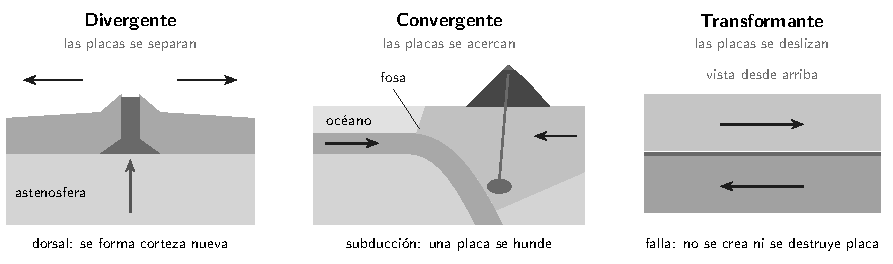
\includegraphics[max width=0.92\linewidth,max height=8.5cm]{fis/tie_limites}
\end{center}
 
\begin{center}\small
\begin{tabularx}{\linewidth}{@{}>{\raggedright\arraybackslash\hsize=0.97\hsize}X>{\raggedright\arraybackslash\hsize=1.10\hsize}X>{\raggedright\arraybackslash\hsize=1.10\hsize}X>{\raggedright\arraybackslash\hsize=0.83\hsize}X@{}}
\toprule
\textbf{Límite} & \textbf{Movimiento} & \textbf{Qué se forma} & \textbf{Ejemplo} \\
\midrule
Divergente & las placas se separan & dorsales, rift, corteza nueva, volcanismo, sismos poco profundos & dorsal mesoatlántica, Islandia \\
Convergente oceánica-continental & se acercan; la oceánica, más densa, se hunde (subducción) & fosa, cordillera, volcanes, sismos de todas las profundidades & Nazca bajo la Sudamericana \\
Convergente continental-continental & se acercan; ninguna se hunde mucho & grandes cordilleras por plegamiento & Himalaya \\
Transformante & se deslizan lateralmente & fallas, sismos; no se crea ni se destruye placa & falla de San Andrés \\
\bottomrule
\end{tabularx}
\end{center}
\subsection{Consecuencias: sismos, volcanismo y relieve en Chile}
Chile está sobre un límite \textbf{convergente}: la \textbf{placa de Nazca}, oceánica, se hunde bajo la \textbf{placa Sudamericana}, continental, a unos 6 a 7 cm por año. De esa subducción resultan:

 
\begin{itemize}
  \item \textbf{Fosa de Chile-Perú:} depresión submarina profunda donde la placa de Nazca empieza a hundirse.
  \item \textbf{Sismos:} las placas se traban en su contacto, acumulan energía y la liberan de golpe. Los hipocentros son más profundos hacia el este, siguiendo la placa que se hunde. Ahí ocurrió el mayor sismo registrado, Valdivia 1960 (magnitud 9,5).
  \item \textbf{Volcanismo:} a unos 100 km de profundidad, la placa que se hunde libera agua que hace fundir parcialmente el manto: se forma magma que asciende y alimenta los volcanes de los Andes.
  \item \textbf{Relieve:} la compresión levanta la cordillera de la Costa y la cordillera de los Andes.
\end{itemize}
  
\begin{center}
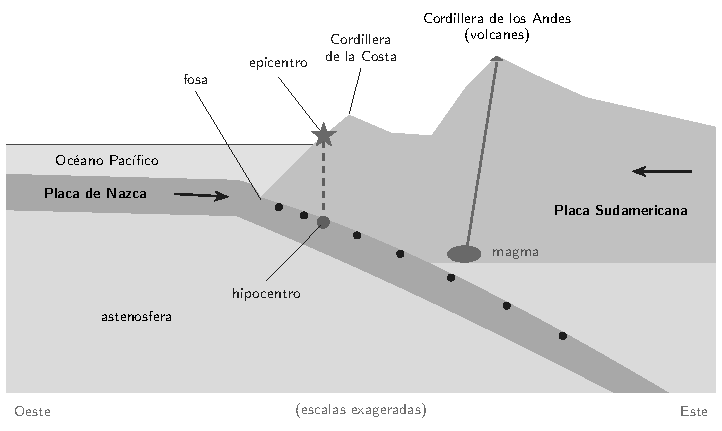
\includegraphics[max width=0.92\linewidth,max height=8.5cm]{fis/tie_chile}
\end{center}
 
\begin{clave}[{Recuerda}] En el extremo sur de Chile el contacto con la placa de Scotia es transformante: las placas se deslizan, hay sismos, pero no se formó una cordillera como los Andes.\end{clave}
\subsection{Lo clave del tema}
\begin{center}\small
\begin{tabularx}{\linewidth}{@{}>{\raggedright\arraybackslash\hsize=0.91\hsize}X>{\raggedright\arraybackslash\hsize=1.04\hsize}X>{\raggedright\arraybackslash\hsize=1.04\hsize}X@{}}
\toprule
\textbf{Idea} & \textbf{Qué dice} & \textbf{Evidencia o ejemplo} \\
\midrule
Deriva continental (Wegener) & los continentes estuvieron unidos en Pangea y se desplazaron & encaje, fósiles, rocas, paleoclimas \\
Expansión del fondo oceánico (Hess) & en las dorsales se forma corteza nueva; en las fosas se destruye & rocas más jóvenes junto a la dorsal, bandas magnéticas simétricas \\
Tectónica de placas & la litosfera está dividida en placas que se mueven sobre la astenosfera & sismos y volcanes concentrados en los bordes de placa \\
Límite divergente & placas se separan & dorsal mesoatlántica \\
Límite convergente & placas se acercan; subducción o colisión & Andes, Himalaya \\
Límite transformante & placas se deslizan lateralmente & San Andrés, Scotia-Sudamericana \\
\bottomrule
\end{tabularx}
\end{center}
 
\begin{clave}[{Recuerda}] · Wegener tenía evidencias, pero no un mecanismo; la tectónica de placas lo aportó.\par · Rocas a igual distancia de la dorsal tienen igual edad; más lejos, más antiguas.\par · Los Andes se formaron por la convergencia de las placas de Nazca y Sudamericana.\end{clave}
 
\begin{clave}[{Método PAES}] 1. Identifica el tipo de límite por el movimiento (se separan, se acercan, se deslizan). 2. Asocia sus consecuencias (dorsal, fosa y cordillera, falla). 3. En preguntas de investigación, busca qué medición responde directamente la pregunta y en qué escala de tiempo (las placas se mueven centímetros por año). 4. Descarta alternativas que no se deducen de los datos.\end{clave}
\begin{elejemplo}{PAES Regular 2026, adaptada}
Un equipo extrae rocas del fondo oceánico a ambos lados de una dorsal. Una roca obtenida a 50 km al oeste del eje de la dorsal tiene 2 millones de años.

Si la expansión del fondo oceánico ha sido constante e igual hacia ambos lados, ¿qué edad se espera para una roca extraída a 100 km al \textbf{este} del eje de la dorsal?
\alts{2 millones de años}{4 millones de años}{1 millón de años}{8 millones de años}
\solucion{\textbf{Paso 1. ¿Qué nos piden?} La edad de una roca del fondo oceánico según su distancia a la dorsal.

\textbf{Paso 2. Recuerda el proceso.} En la dorsal se forma roca nueva que se desplaza hacia ambos lados. Si la expansión es constante y simétrica, la edad de una roca es proporcional a su distancia al eje, sin importar de qué lado esté.

\textbf{Paso 3. Calcula.} A 50 km la roca tiene 2 millones de años. A 100 km, el doble de distancia, la roca tiene el doble de edad: 4 millones de años. De paso, la rapidez de expansión es $\dfrac{50 \text{ km}}{2 \text{ millones de años}}$, es decir, 2,5 cm por año.

\textbf{Respuesta:} 4 millones de años.

\textbf{¿Por qué no las otras?} 2 millones de años correspondería a una roca a 50 km del eje, hacia cualquiera de los lados. 1 millón de años invierte la relación: más lejos significa más antigua, no más joven. 8 millones de años supone que la edad crece con el cuadrado de la distancia.

\textbf{\color{cienciaD}Para recordar.} En una dorsal, la edad de la roca crece con la distancia al eje, igual hacia ambos lados.}{B}
\end{elejemplo}

%% =====================================================================
%% fis_interior
\section[Interior de la Tierra y sismos]{Interior de la Tierra y sismos}
\modcomun\ \ {\color{gris}\itshape Los modelos estático (corteza, manto y núcleo) y dinámico (litosfera, astenosfera, mesosfera y núcleo externo e interno) de la geosfera, las ondas sísmicas P y S, hipocentro y epicentro, magnitud e intensidad de un sismo y la energía que libera.\par}
\subsection{Dos modelos de la geosfera}
El interior de la Tierra se describe con dos modelos que se complementan:

 

\textbf{Modelo estático} (según la \textbf{composición química}):

 
\begin{itemize}
  \item \textbf{Corteza:} continental (5 a 70 km de espesor, rocas como el granito) u oceánica (5 a 10 km, basalto).
  \item \textbf{Manto:} hasta unos 2900 km; rocas de silicatos de hierro y magnesio.
  \item \textbf{Núcleo:} hasta el centro, a 6371 km; principalmente hierro y níquel.
\end{itemize}
 

\textbf{Modelo dinámico} (según el \textbf{comportamiento físico}: rígido, plástico o líquido):

 
\begin{itemize}
  \item \textbf{Litosfera:} rígida; corteza más la parte superior del manto, unos 100 km. Está dividida en placas.
  \item \textbf{Astenosfera:} parte del manto superior que se comporta como un material \textbf{plástico}: es sólida, pero fluye muy lentamente.
  \item \textbf{Mesosfera:} manto inferior, sólido, hasta los 2900 km.
  \item \textbf{Núcleo externo:} \textbf{líquido}, hasta unos 5150 km. Sus movimientos generan el campo magnético terrestre.
  \item \textbf{Núcleo interno:} \textbf{sólido}, por la enorme presión, aunque su temperatura supera los 5000 °C.
\end{itemize}
  
\begin{center}
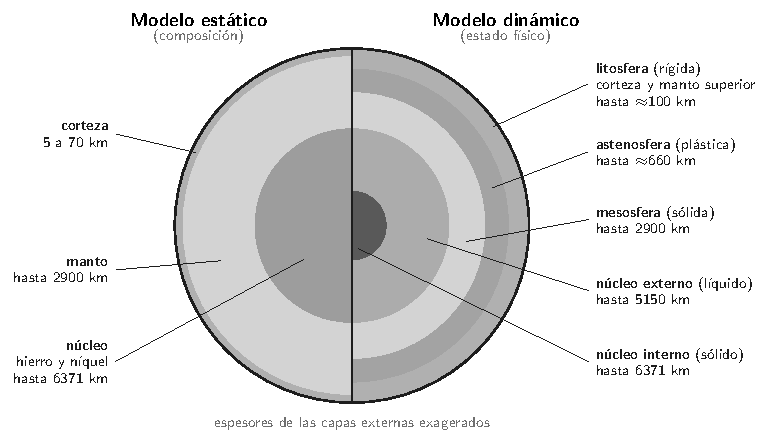
\includegraphics[max width=0.92\linewidth,max height=8.5cm]{fis/tie_capas}
\end{center}
 
\begin{clave}[{Recuerda}] La litosfera no es lo mismo que la corteza: incluye la corteza y una parte del manto. Y la astenosfera no es un océano de roca fundida: es roca sólida que se deforma lentamente.\end{clave}
\subsection{¿Cómo conocemos el interior? Las ondas sísmicas}
La perforación más profunda llega a unos 12 km. Todo lo demás se sabe estudiando cómo viajan las \textbf{ondas sísmicas}: su rapidez cambia según el material, y en los límites entre capas se reflejan y se refractan (cambian de dirección).

 
\begin{itemize}
  \item \textbf{Ondas P} (primarias): \textbf{longitudinales}, de compresión. Son las \textbf{más rápidas} (unos 6 km/s en la corteza) y viajan por sólidos, líquidos y gases.
  \item \textbf{Ondas S} (secundarias): \textbf{transversales}. Son más lentas (unos 3,5 km/s en la corteza) y \textbf{solo viajan por sólidos}.
  \item \textbf{Ondas superficiales:} viajan por la superficie, son las más lentas y las que más daño causan.
\end{itemize}
  
\begin{center}
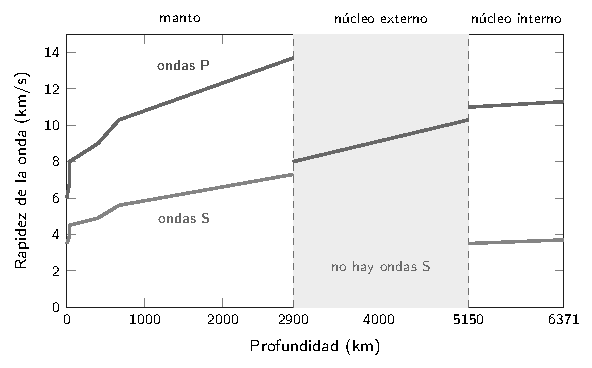
\includegraphics[max width=0.92\linewidth,max height=8.5cm]{fis/tie_velocidades}
\end{center}
 
\begin{clave}[{La gran pista}] A los 2900 km las ondas S \textbf{dejan de propagarse} y las ondas P se frenan bruscamente. Como las ondas S no viajan por líquidos, el \textbf{núcleo externo es líquido}. Por eso, en el lado opuesto de la Tierra al sismo existe una zona de sombra donde no llegan ondas S directas.\end{clave}
\subsection{Los sismos: hipocentro, epicentro y energía}
En los bordes de placa, las rocas quedan \textbf{trabadas} por el roce. Mientras las placas siguen moviéndose, las rocas se deforman y acumulan \textbf{energía elástica}, como un resorte que se comprime. Cuando la tensión supera la resistencia de la roca, esta se rompe y se desliza de golpe: la energía acumulada se libera como \textbf{ondas sísmicas}, calor y deformación del terreno. Eso es un \textbf{sismo}.

 
\begin{itemize}
  \item \textbf{Hipocentro} (o foco): punto en el interior de la Tierra donde se inicia la ruptura.
  \item \textbf{Epicentro:} punto de la \textbf{superficie} ubicado justo encima del hipocentro.
\end{itemize}
 

Si el epicentro está en el mar y el sismo levanta bruscamente el fondo oceánico, puede generar un \textbf{tsunami}.

  
\begin{center}
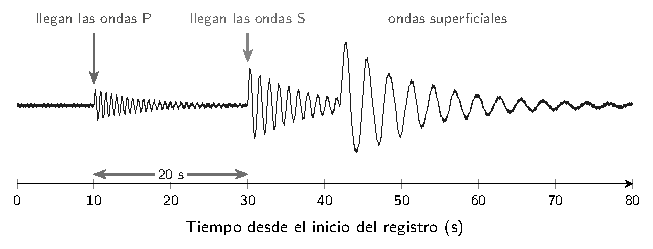
\includegraphics[max width=0.92\linewidth,max height=8.5cm]{fis/tie_sismograma}
\end{center}
 
\begin{clave}[{Distancia al sismo}] Las ondas P llegan primero porque son más rápidas. Mientras más lejos está la estación, mayor es el tiempo entre la llegada de las P y la de las S. Con ese intervalo se calcula la distancia al hipocentro, y con tres estaciones se ubica el epicentro.\end{clave}
\subsection{Magnitud e intensidad}
\textbf{Magnitud:} mide la \textbf{energía liberada} en el hipocentro. Cada sismo tiene \textbf{una sola magnitud}, que se calcula con los registros de los sismógrafos. Se usan la escala de Richter y, para sismos grandes, la escala de magnitud de momento (Mw). Son escalas \textbf{logarítmicas}: un grado más de magnitud significa unas \textbf{32 veces más energía}, y dos grados, unas 1000 veces más.

 

\textbf{Intensidad:} mide los \textbf{efectos} del sismo en un lugar: cómo lo percibieron las personas y qué daños produjo. Se expresa con la \textbf{escala de Mercalli}, de I a XII en números romanos. Un mismo sismo tiene \textbf{distintas intensidades} en distintos lugares: depende de la distancia al epicentro, de la profundidad, del tipo de suelo y de la calidad de las construcciones.

  
\begin{center}\small
\begin{tabularx}{\linewidth}{@{}>{\raggedright\arraybackslash\hsize=0.65\hsize}X>{\raggedright\arraybackslash\hsize=1.13\hsize}X>{\raggedright\arraybackslash\hsize=1.22\hsize}X@{}}
\toprule
 & \textbf{Magnitud} & \textbf{Intensidad} \\
\midrule
Qué mide & energía liberada & efectos y daños en un lugar \\
Cuántos valores & uno por sismo & uno por cada lugar \\
Escala & Richter o Mw (logarítmica) & Mercalli (I a XII) \\
Cómo se obtiene & con sismógrafos & con observaciones de efectos \\
\bottomrule
\end{tabularx}
\end{center}
 
\begin{ejemplo}[{Ejemplos chilenos}] Valdivia, 1960: magnitud 9,5, el mayor sismo registrado. Maule, 2010: magnitud 8,8, con un tsunami que afectó la costa centro-sur.\end{ejemplo}
\subsection{Lo clave del tema}
\begin{center}\small
\begin{tabularx}{\linewidth}{@{}>{\raggedright\arraybackslash\hsize=0.65\hsize}X>{\raggedright\arraybackslash\hsize=1.18\hsize}X>{\raggedright\arraybackslash\hsize=1.18\hsize}X@{}}
\toprule
\textbf{Concepto} & \textbf{Qué es} & \textbf{Dato clave} \\
\midrule
Modelo estático & capas según composición & corteza, manto, núcleo \\
Modelo dinámico & capas según comportamiento físico & litosfera rígida, astenosfera plástica, núcleo externo líquido \\
Ondas P & longitudinales, las más rápidas & viajan por sólidos y líquidos \\
Ondas S & transversales, más lentas & solo por sólidos: no cruzan el núcleo externo \\
Hipocentro y epicentro & origen interior y punto de superficie encima & el epicentro está sobre el hipocentro \\
Magnitud & energía liberada & una por sismo; +1 grado \ensuremath{\approx} 32 veces más energía \\
Intensidad & efectos en un lugar & Mercalli; cambia de un lugar a otro \\
\bottomrule
\end{tabularx}
\end{center}
 
\begin{clave}[{Recuerda}] · Si las ondas S desaparecen, la capa es líquida.\par · La litosfera incluye la corteza y parte del manto.\par · Un sismo tiene una magnitud y muchas intensidades.\end{clave}
 
\begin{clave}[{Método PAES}] 1. Distingue si la pregunta es de composición (modelo estático) o de comportamiento físico (modelo dinámico). 2. En gráficos de ondas, busca dónde cambian o desaparecen. 3. Para magnitud o intensidad, pregúntate si se habla de energía o de efectos. 4. En preguntas de investigación, busca el dato que se relaciona directamente con lo que se quiere saber.\end{clave}
\begin{elejemplo}{Estilo PAES}
Una estación sismológica registra un sismo. Las ondas S llegan 20 segundos después que las ondas P, como muestra el sismograma. En la zona, las ondas P viajan a 6 km/s y las ondas S a 4 km/s.

¿A qué distancia aproximada de la estación se originó el sismo?
\begin{center}
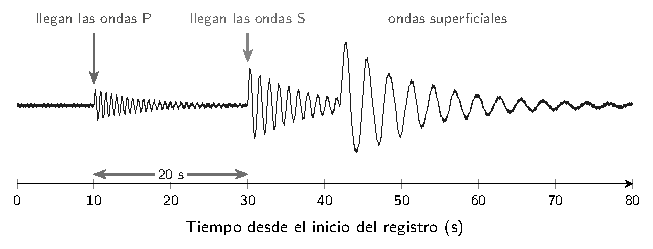
\includegraphics[max width=0.92\linewidth,max height=8.5cm]{fis/tie_sismograma}
\end{center}
\alts{120 km}{80 km}{200 km}{240 km}
\solucion{\textbf{Paso 1. ¿Qué nos piden?} La distancia $d$ al origen del sismo, a partir del retraso de las ondas S respecto de las P.

\textbf{Paso 2. Plantea los tiempos.} Ambas ondas recorren la misma distancia $d$ con rapidez constante, así que $t_P = \dfrac{d}{6}$ y $t_S = \dfrac{d}{4}$ (en segundos, con $d$ en km).

\textbf{Paso 3. Usa la diferencia.} $t_S - t_P = \dfrac{d}{4} - \dfrac{d}{6} = \dfrac{3d - 2d}{12} = \dfrac{d}{12}$. Como la diferencia es 20 s: $\dfrac{d}{12} = 20$, entonces $d = 240$ km.

\textbf{Comprobación:} $t_P = 240/6 = 40$ s y $t_S = 240/4 = 60$ s; la diferencia es 20 s. \ding{52}

\textbf{Respuesta:} 240 km.

\textbf{¿Por qué no las otras?} 120 km resulta de multiplicar 20 s por la rapidez de las ondas P, como si las P hubieran tardado 20 s en llegar. 80 km hace lo mismo con la rapidez de las S. 200 km resulta de multiplicar 20 s por la suma de las rapideces, que no tiene sentido físico.

\textbf{\color{cienciaD}Para recordar.} El retraso de las ondas S respecto de las P crece con la distancia: d/vS \ensuremath{-} d/vP = \ensuremath{\Delta}t.}{D}
\end{elejemplo}

\chapter{Electricidad}
%% =====================================================================
%% fis_corriente_ohm
\section[Corriente eléctrica y ley de Ohm]{Corriente eléctrica y ley de Ohm}
\modcomun\ \ {\color{gris}\itshape Qué es la corriente eléctrica y cómo se calcula (I = q/t), su sentido convencional, el voltaje y la resistencia, la ley de Ohm (V = I·R), la lectura de gráficos V--I (la pendiente es la resistencia), conductores óhmicos y no óhmicos, y cómo se conectan el amperímetro y el voltímetro.\par}
\subsection{La corriente eléctrica}
La materia está formada por partículas con \textbf{carga eléctrica}: protones (positivos) y electrones (negativos). La carga se mide en \textbf{coulomb} (C). En los metales, algunos electrones se pueden mover con libertad por el material.

 

La \textbf{corriente eléctrica} es un flujo ordenado de cargas a través de un conductor. Su \textbf{intensidad} $I$ indica cuánta carga $q$ atraviesa una sección del conductor en cada unidad de tiempo:

 \[ I = \dfrac{q}{t} \] 

Se mide en \textbf{ampere} (A): 1 A = 1 C/s. Si por un cable pasan 6 C en 3 s, la intensidad es $I = 6/3 = 2$ A.

 

Para que circule corriente se necesita un \textbf{circuito cerrado}: un camino conductor continuo que sale de la fuente (pila, batería, enchufe) y vuelve a ella. Si el circuito se abre en algún punto (un interruptor apagado, un cable cortado), la corriente se detiene en todo ese camino.

  
\begin{clave}[{Sentido de la corriente}] En un cable metálico, los electrones se mueven por el circuito externo desde el polo negativo hacia el polo positivo de la pila. Por una convención histórica, el \textbf{sentido convencional} de la corriente es el contrario: sale del polo \textbf{positivo}, recorre el circuito y vuelve por el polo \textbf{negativo}. Las flechas de corriente de los diagramas usan el sentido convencional.\end{clave}
 
\begin{clave}[{Recuerda}] · La corriente no se «gasta» al pasar por una ampolleta: la misma carga que entra por un extremo sale por el otro. Lo que la ampolleta transforma es \textbf{energía}.\par · Las pilas y baterías entregan \textbf{corriente continua} (siempre en el mismo sentido). La red domiciliaria entrega \textbf{corriente alterna}, que en Chile cambia de sentido 50 veces por segundo.\end{clave}
\subsection{Voltaje y resistencia}
La \textbf{diferencia de potencial} o \textbf{voltaje} $V$ es la energía que la fuente entrega a cada unidad de carga que pasa por ella. Se mide en \textbf{volt} (V): 1 V = 1 J/C. Una pila de 1,5 V entrega 1,5 J a cada coulomb; la red domiciliaria chilena tiene 220 V.

 

El voltaje es lo que impulsa a las cargas. Una analogía útil es el agua: la diferencia de altura entre dos estanques hace que el agua fluya por un tubo; el voltaje hace que la carga fluya por el cable.

 

La \textbf{resistencia eléctrica} $R$ mide cuánto se opone un elemento al paso de la corriente. Se mide en \textbf{ohm} (\ensuremath{\Omega}). Al atravesar una resistencia, la energía eléctrica se transforma en calor (efecto Joule), y en el filamento de una ampolleta también en luz.

  
\begin{clave}[{De qué depende la resistencia de un cable}] · Del \textbf{material}: el cobre conduce muy bien; el nicrom, que se usa en estufas, mucho peor.\par · Del \textbf{largo}: a mayor largo, mayor resistencia.\par · Del \textbf{área de la sección} (el grosor): a mayor grosor, menor resistencia.\par · De la \textbf{temperatura}: en los metales, la resistencia aumenta al calentarse.\end{clave}
 

En la analogía del agua, un tubo largo y delgado deja pasar menos agua por segundo que uno corto y ancho, con la misma diferencia de altura.

 
\begin{clave}[{Recuerda}] Los conductores (metales, grafito, agua con sales disueltas) tienen resistencia baja. Los aislantes (plástico, goma, vidrio, aire seco) tienen resistencia muy alta.\end{clave}
\subsection{Ley de Ohm}
En muchos conductores, si la temperatura se mantiene, la corriente es \textbf{directamente proporcional} al voltaje aplicado. Es la \textbf{ley de Ohm}:

 \[ V = I\cdot R \] 

Despejando se obtiene $I = \dfrac{V}{R}$ y $R = \dfrac{V}{I}$.

 

\textbf{Ejemplo 1.} Un hervidor tiene una resistencia de 22 \ensuremath{\Omega} y se conecta a 220 V: $I = 220/22 = 10$ A.

 

\textbf{Ejemplo 2.} Por un resistor circulan 0,5 A cuando se le aplican 6 V: $R = 6/0{,}5 = 12$ \ensuremath{\Omega}.

  
\begin{clave}[{Cómo leer la ley}] · Con la misma resistencia, si el voltaje se duplica, la corriente se duplica.\par · Con el mismo voltaje, si la resistencia se duplica, la corriente se reduce a la mitad.\par · Para aumentar la corriente: aumenta el voltaje o disminuye la resistencia.\end{clave}
 
\begin{clave}[{Recuerda}] Usa las unidades base: $V$ en volt, $I$ en ampere y $R$ en ohm. Si te dan miliampere, conviértelos: 200 mA = 0,2 A. Si te dan kiloohm: 2 k\ensuremath{\Omega} = 2000 \ensuremath{\Omega}.\end{clave}
\subsection{Gráficos V--I: conductores óhmicos y no óhmicos}
Si se mide la corriente para distintos voltajes y se grafica $V$ en función de $I$, un \textbf{conductor óhmico} da una \textbf{recta que pasa por el origen}. Su \textbf{pendiente es la resistencia}:

 \[ R = \dfrac{\Delta V}{\Delta I} \] 

En el gráfico, la recta azul pasa por (1 A; 10 V): su resistencia es 10 \ensuremath{\Omega}, la misma en cualquier punto.

 

Un \textbf{conductor no óhmico} no da una recta: su resistencia cambia con el voltaje. El filamento de una ampolleta se calienta cuando aumenta la corriente, y su resistencia aumenta: con 0,5 A tiene $3{,}5/0{,}5 = 7$ \ensuremath{\Omega}, y con 1 A tiene $10/1 = 10$ \ensuremath{\Omega}. Los diodos y los LED también son no óhmicos.

  
\begin{center}
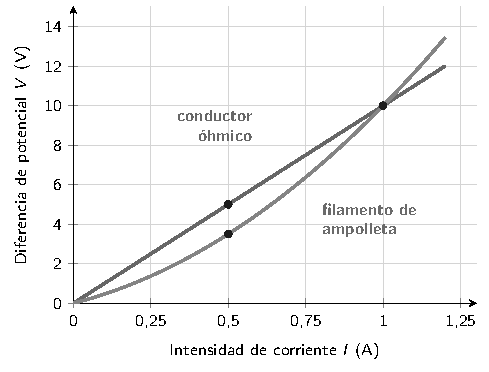
\includegraphics[max width=0.92\linewidth,max height=8.5cm]{fis/ele_vi_curva}
\end{center}
 
\begin{clave}[{Fíjate en los ejes}] Si el gráfico es de $I$ en función de $V$ (la corriente en el eje vertical), la pendiente es $\dfrac{1}{R}$: la resistencia es el \textbf{inverso de la pendiente}. En ese gráfico, la recta más inclinada es la de \textbf{menor} resistencia.\end{clave}
\subsection{Cómo medir corriente y voltaje}
El \textbf{amperímetro} mide la intensidad de corriente. Se conecta \textbf{en serie}: se abre el circuito y se intercala el instrumento, para que toda la corriente pase a través de él. Un buen amperímetro tiene una resistencia muy pequeña, para no alterar la corriente que mide.

 

El \textbf{voltímetro} mide la diferencia de potencial entre dos puntos. Se conecta \textbf{en paralelo} con el elemento, tocando sus dos extremos. Un buen voltímetro tiene una resistencia muy grande, para que casi no pase corriente por él.

 

El \textbf{óhmetro} mide resistencias, con el elemento desconectado del circuito. El \textbf{multímetro} (o tester) reúne los tres instrumentos.

  
\begin{center}
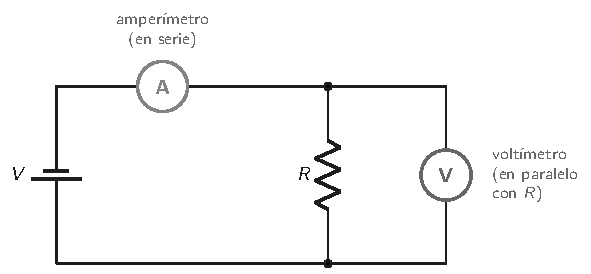
\includegraphics[max width=0.92\linewidth,max height=8.5cm]{fis/ele_medicion}
\end{center}
 
\begin{clave}[{Recuerda}] · Amperímetro: en serie, dentro del camino de la corriente.\par · Voltímetro: en paralelo, entre los extremos del elemento.\par · Para obtener una resistencia de forma experimental, mide $V$ con el voltímetro, mide $I$ con el amperímetro y calcula $R = V/I$.\end{clave}
\subsection{Lo clave del tema}
\begin{center}\small
\begin{tabularx}{\linewidth}{@{}>{\raggedright\arraybackslash\hsize=1.10\hsize}X>{\raggedright\arraybackslash\hsize=0.48\hsize}X>{\raggedright\arraybackslash\hsize=0.52\hsize}X>{\raggedright\arraybackslash\hsize=1.90\hsize}X@{}}
\toprule
\textbf{Magnitud} & \textbf{Símbolo} & \textbf{Unidad} & \textbf{Idea clave} \\
\midrule
Carga eléctrica & $q$ & coulomb (C) & propiedad de protones y electrones \\
Intensidad de corriente & $I$ & ampere (A) & $I = q/t$; se mide con amperímetro en serie \\
Voltaje & $V$ & volt (V) & energía por unidad de carga; se mide con voltímetro en paralelo \\
Resistencia & $R$ & ohm (\ensuremath{\Omega}) & aumenta con el largo y la temperatura; disminuye con el grosor \\
Ley de Ohm & \multicolumn{2}{@{}l@{}}{$V = I\cdot R$} & con $R$ constante, $I$ es proporcional a $V$ \\
Gráfico V--I óhmico & \multicolumn{2}{@{}l@{}}{recta por el origen} & pendiente de $V$ vs $I$ = $R$; pendiente de $I$ vs $V$ = $1/R$ \\
\bottomrule
\end{tabularx}
\end{center}
 
\begin{clave}[{Recuerda}] · La corriente no se gasta: lo que se transforma es la energía.\par · El sentido convencional va del polo positivo al negativo por el circuito externo; los electrones van al revés.\par · Un conductor no óhmico (filamento, LED) da una curva: su resistencia cambia.\end{clave}
 
\begin{clave}[{Método PAES}] 1. Anota los datos con sus unidades y conviértelas (mA a A, minutos a segundos). 2. Elige la fórmula: $I = q/t$ o $V = I\cdot R$. 3. En un gráfico, mira qué va en cada eje antes de usar la pendiente. 4. Revisa si el resultado tiene sentido: más voltaje, más corriente; más resistencia, menos corriente.\end{clave}
\begin{elejemplo}{PAES Invierno 2027, adaptada}
Un grupo de estudiantes conecta, por separado, dos resistencias óhmicas a una fuente de voltaje variable y mide la intensidad de corriente para distintos voltajes. Con los datos construye el gráfico de la figura.

Si se aplica una diferencia de potencial de 12 V a la resistencia 2, ¿qué intensidad de corriente circula por ella?
\begin{center}
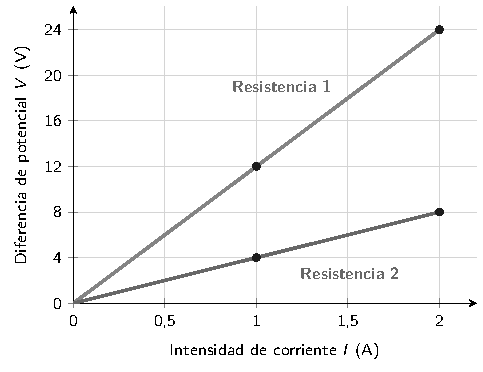
\includegraphics[max width=0.92\linewidth,max height=8.5cm]{fis/ele_vi}
\end{center}
\alts{1 A}{3 A}{48 A}{0,33 A}
\solucion{\textbf{Paso 1. ¿Qué nos piden?} La corriente en la resistencia 2 cuando se le aplican 12 V.

\textbf{Paso 2. Obtén la resistencia con la pendiente.} En un gráfico de $V$ en función de $I$, la pendiente es la resistencia. La recta 2 pasa por (2 A; 8 V): $R_2 = \dfrac{8}{2} = 4$ \ensuremath{\Omega}.

\textbf{Paso 3. Aplica la ley de Ohm.} La resistencia es óhmica (su gráfico es una recta por el origen), así que mantiene sus 4 \ensuremath{\Omega} aunque el voltaje sea mayor que los medidos: $I = \dfrac{V}{R} = \dfrac{12}{4} = 3$ A.

\textbf{Respuesta:} 3 A.

\textbf{¿Por qué no las otras?} 1 A es el resultado de usar la resistencia 1 (12 \ensuremath{\Omega}) en lugar de la 2. 48 A sale de multiplicar el voltaje por la resistencia, en vez de dividir. 0,33 A sale de dividir la resistencia por el voltaje.

\textbf{\color{cienciaD}Para recordar.} En un gráfico V--I, la pendiente es la resistencia; con ella, la ley de Ohm da la corriente.}{B}
\end{elejemplo}

%% =====================================================================
%% fis_circuitos
\section[Circuitos en serie, paralelo y mixtos]{Circuitos en serie, paralelo y mixtos}
\modcomun\ \ {\color{gris}\itshape Cómo se reparten la corriente y el voltaje en circuitos en serie y en paralelo, la resistencia equivalente, qué pasa al desconectar o fundir una ampolleta, el brillo relativo de ampolletas iguales, la ley de nudos y la resolución de circuitos mixtos.\par}
\subsection{Circuito en serie}
En un circuito \textbf{en serie} los elementos están uno a continuación del otro: la corriente tiene \textbf{un solo camino}.

 
\begin{itemize}
  \item \textbf{Corriente:} es la \textbf{misma} en todos los elementos.
  \item \textbf{Voltaje:} el de la fuente se \textbf{reparte} entre los elementos: $V = V_1 + V_2 + \dots$ El de mayor resistencia recibe más voltaje, porque $V_i = I\cdot R_i$.
  \item \textbf{Resistencia equivalente:} las resistencias se suman: $R_{\text{eq}} = R_1 + R_2 + \dots$ Siempre es mayor que la mayor de ellas.
\end{itemize}
 

\textbf{Ejemplo.} Resistencias de 2 \ensuremath{\Omega}, 4 \ensuremath{\Omega} y 6 \ensuremath{\Omega} en serie con una batería de 24 V: $R_{\text{eq}} = 12$ \ensuremath{\Omega} e $I = 24/12 = 2$ A. Los voltajes son $2\cdot 2 = 4$ V, $2\cdot 4 = 8$ V y $2\cdot 6 = 12$ V, que suman 24 V.

  
\begin{center}
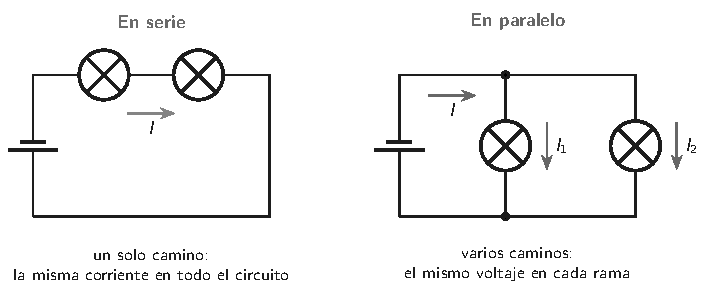
\includegraphics[max width=0.92\linewidth,max height=8.5cm]{fis/ele_serie_paralelo}
\end{center}
 
\begin{clave}[{Recuerda}] Si una ampolleta en serie se funde o se desconecta, el circuito se abre y \textbf{todas se apagan}. Al agregar más elementos en serie, la resistencia total aumenta y la corriente disminuye.\end{clave}
\subsection{Circuito en paralelo}
En un circuito \textbf{en paralelo} cada elemento se conecta directamente a los dos extremos de la fuente: la corriente tiene \textbf{varios caminos}, llamados ramas.

 
\begin{itemize}
  \item \textbf{Voltaje:} es el \textbf{mismo} en todas las ramas e igual al de la fuente.
  \item \textbf{Corriente:} la total se \textbf{reparte} entre las ramas: $I = I_1 + I_2 + \dots$ Por la rama de menor resistencia pasa más corriente.
  \item \textbf{Resistencia equivalente:} $\dfrac{1}{R_{\text{eq}}} = \dfrac{1}{R_1} + \dfrac{1}{R_2} + \dots$ Siempre es menor que la menor de ellas.
\end{itemize}
 

\textbf{Ejemplo.} Resistencias de 6 \ensuremath{\Omega} y 3 \ensuremath{\Omega} en paralelo con 12 V: $I_1 = 12/6 = 2$ A e $I_2 = 12/3 = 4$ A, así que $I = 6$ A y $R_{\text{eq}} = 12/6 = 2$ \ensuremath{\Omega}. Con la fórmula: $\dfrac{1}{R_{\text{eq}}} = \dfrac{1}{6} + \dfrac{1}{3} = \dfrac{3}{6}$, de donde $R_{\text{eq}} = 2$ \ensuremath{\Omega}.

  
\gatotip[\gatonegro]{\textbf{Atajos.} · Dos resistencias: $R_{\text{eq}} = \dfrac{R_1\cdot R_2}{R_1 + R_2}$.\par · $n$ resistencias iguales de valor $R$: $R_{\text{eq}} = \dfrac{R}{n}$.}
 
\begin{clave}[{Recuerda}] Si una rama se desconecta, las demás siguen funcionando igual (mismo voltaje, misma corriente), pero la corriente total que entrega la fuente disminuye. Al agregar ramas, la resistencia total disminuye y la corriente total aumenta. Por eso la instalación de una casa es en paralelo: cada artefacto funciona de forma independiente.\end{clave}
\subsection{Brillo de las ampolletas}
El brillo de una ampolleta depende de la \textbf{potencia} que disipa: $P = V\cdot I = I^2\cdot R = \dfrac{V^2}{R}$. Si las ampolletas son \textbf{iguales}, brilla más la que tiene \textbf{más corriente} (y, por lo tanto, más voltaje).

 

\textbf{En serie.} Dos ampolletas iguales en serie reciben la mitad del voltaje cada una: brillan menos que una sola conectada a la misma pila.

 

\textbf{En paralelo.} Cada ampolleta recibe el voltaje completo y brilla igual que si estuviera sola. A cambio, la pila entrega más corriente y se descarga antes.

 

\textbf{Circuito de la figura} (tres ampolletas iguales). Toda la corriente pasa por $L_1$ y luego se divide en partes iguales entre $L_2$ y $L_3$. Por eso $L_1$ brilla más, y $L_2$ y $L_3$ brillan igual entre sí.

  
\begin{center}
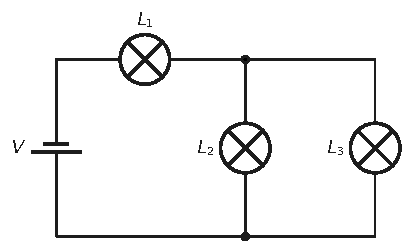
\includegraphics[max width=0.92\linewidth,max height=8.5cm]{fis/ele_brillo}
\end{center}
 
\begin{clave}[{Si se funde L3}] La resistencia total pasa de $R + \dfrac{R}{2} = 1{,}5R$ a $2R$: la corriente total disminuye y $L_1$ brilla menos. Toda esa corriente pasa ahora por $L_2$: antes recibía $\dfrac{V}{3R}$ y ahora recibe $\dfrac{V}{2R}$, así que $L_2$ brilla más.\end{clave}
\subsection{Circuitos mixtos}
Un circuito \textbf{mixto} combina partes en serie y partes en paralelo. Se resuelve por etapas, reemplazando grupos de resistencias por su equivalente:

 
\begin{enumerate}
  \item Reemplaza cada grupo en paralelo por su resistencia equivalente.
  \item Suma las resistencias que quedan en serie: obtienes $R_{\text{eq}}$.
  \item Calcula la corriente total: $I = V/R_{\text{eq}}$.
  \item Vuelve atrás: calcula el voltaje de cada parte y la corriente de cada rama.
\end{enumerate}
 

\textbf{En la figura.} $R_2$ y $R_3$ están en paralelo: $\dfrac{6\cdot 3}{6 + 3} = 2$ \ensuremath{\Omega}. En serie con $R_1$: $R_{\text{eq}} = 2 + 2 = 4$ \ensuremath{\Omega}. Corriente total: $I = 12/4 = 3$ A, que pasa entera por $R_1$. Voltaje en $R_1$: $3\cdot 2 = 6$ V, así que al paralelo le quedan 6 V. Corrientes: $6/6 = 1$ A por $R_2$ y $6/3 = 2$ A por $R_3$.

  
\begin{center}
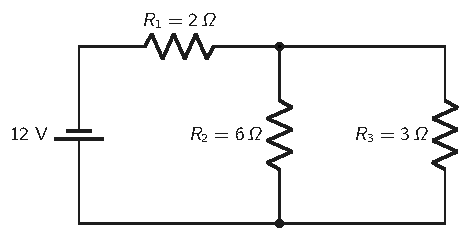
\includegraphics[max width=0.92\linewidth,max height=8.5cm]{fis/ele_mixto}
\end{center}
 
\begin{clave}[{Comprueba siempre}] Los voltajes de los tramos en serie suman el de la fuente (6 V + 6 V = 12 V), y las corrientes de las ramas suman la corriente total (1 A + 2 A = 3 A).\end{clave}
\subsection{Ley de nudos y lectura de datos}
Un \textbf{nudo} es un punto donde se unen tres o más cables. Como la carga no se crea ni se destruye, la corriente que \textbf{entra} a un nudo es igual a la que \textbf{sale} de él:

 \[ \sum I_{\text{entran}} = \sum I_{\text{salen}} \] 

Si a un nudo llegan 3 A y salen por dos ramas, y por una de ellas pasan 1,2 A, por la otra pasan $3 - 1{,}2 = 1{,}8$ A.

 

La corriente que entrega la batería es la suma de las corrientes de las ramas que salen del nudo conectado a ella.

  
\begin{clave}[{Inferir el tipo de conexión desde los datos}] · Si dos elementos tienen siempre la \textbf{misma corriente} y voltajes distintos, están en \textbf{serie}.\par · Si tienen siempre el \textbf{mismo voltaje} y corrientes distintas, están en \textbf{paralelo}.\par · En serie, el de mayor resistencia tiene más voltaje. En paralelo, el de mayor resistencia tiene menos corriente.\end{clave}
 
\begin{clave}[{Recuerda}] En serie se reparte el voltaje y la corriente es la misma. En paralelo se reparte la corriente y el voltaje es el mismo.\end{clave}
\subsection{Lo clave del tema}
\begin{center}\small
\begin{tabularx}{\linewidth}{@{}>{\raggedright\arraybackslash\hsize=0.82\hsize}X>{\raggedright\arraybackslash\hsize=0.99\hsize}X>{\raggedright\arraybackslash\hsize=1.19\hsize}X@{}}
\toprule
 & \textbf{En serie} & \textbf{En paralelo} \\
\midrule
Caminos para la corriente & uno solo & uno por rama \\
Corriente & la misma en todos & se reparte: $I = I_1 + I_2 + \dots$ \\
Voltaje & se reparte: $V = V_1 + V_2 + \dots$ & el mismo en todas las ramas \\
Resistencia equivalente & $R_1 + R_2 + \dots$ (mayor que cada una) & $\dfrac{1}{R_{\text{eq}}} = \dfrac{1}{R_1} + \dfrac{1}{R_2} + \dots$ (menor que cada una) \\
Al agregar un elemento & $R_{\text{eq}}$ aumenta, $I$ disminuye & $R_{\text{eq}}$ disminuye, $I$ total aumenta \\
Si un elemento se funde & se apagan todos & los demás siguen igual \\
\bottomrule
\end{tabularx}
\end{center}
 
\begin{clave}[{Recuerda}] · Con ampolletas iguales, brilla más la que lleva más corriente.\par · En un nudo, la corriente que entra es igual a la que sale.\par · En un circuito mixto, reduce primero los grupos en paralelo.\end{clave}
 
\begin{clave}[{Método PAES}] 1. Identifica qué elementos están en serie (mismo camino) y cuáles en paralelo (mismos dos nudos). 2. Calcula la resistencia equivalente por etapas. 3. Obtén la corriente total con $I = V/R_{\text{eq}}$. 4. Vuelve atrás para repartir voltajes y corrientes. 5. Comprueba: voltajes en serie suman el total; corrientes de las ramas suman la total.\end{clave}
\begin{elejemplo}{Estilo PAES}
En el circuito de la figura, la batería entrega una diferencia de potencial de 12 V.

¿Cuál es la intensidad de corriente que circula por la resistencia $R_3$?
\begin{center}
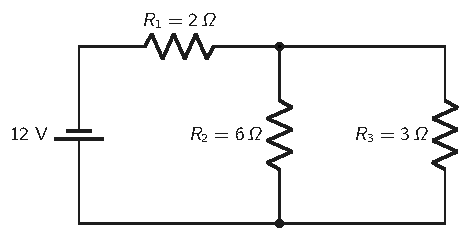
\includegraphics[max width=0.92\linewidth,max height=8.5cm]{fis/ele_mixto}
\end{center}
\alts{3 A}{1 A}{4 A}{2 A}
\solucion{\textbf{Paso 1. ¿Qué nos piden?} La corriente en una de las ramas del paralelo.

\textbf{Paso 2. Reduce el paralelo.} $R_2$ y $R_3$ en paralelo: $\dfrac{6\cdot 3}{6 + 3} = 2$ \ensuremath{\Omega}.

\textbf{Paso 3. Resistencia equivalente y corriente total.} En serie con $R_1$: $R_{\text{eq}} = 2 + 2 = 4$ \ensuremath{\Omega}. $I = \dfrac{12}{4} = 3$ A.

\textbf{Paso 4. Voltaje del paralelo.} En $R_1$ caen $3\cdot 2 = 6$ V; quedan $12 - 6 = 6$ V para $R_2$ y $R_3$.

\textbf{Paso 5. Corriente en $R_3$.} $I_3 = \dfrac{6}{3} = 2$ A. Comprobación: por $R_2$ pasa $6/6 = 1$ A, y $1 + 2 = 3$ A, la corriente total.

\textbf{Respuesta:} 2 A.

\textbf{¿Por qué no las otras?} 3 A es la corriente total, que se divide entre las dos ramas. 1 A es la corriente de $R_2$. 4 A sale de aplicar los 12 V completos a $R_3$, olvidando que una parte del voltaje queda en $R_1$.

\textbf{\color{cienciaD}Para recordar.} En un circuito mixto: reduce, calcula la corriente total y vuelve atrás para repartir.}{D}
\end{elejemplo}

%% =====================================================================
%% fis_potencia
\section[Potencia, energía y consumo eléctrico]{Potencia, energía y consumo eléctrico}
\modcomun\ \ {\color{gris}\itshape Potencia eléctrica (P = V·I = I²·R = V²/R), energía consumida en joule y en kWh, cálculo del costo de la cuenta de la luz y los componentes de la instalación eléctrica de una casa: medidor, tablero, diferencial, conexión a tierra y enchufes en paralelo.\par}
\subsection{Potencia eléctrica}
La \textbf{potencia eléctrica} $P$ es la energía que un artefacto transforma en cada segundo. Se mide en \textbf{watt} (W): 1 W = 1 J/s.

 \[ P = V\cdot I \] 

Combinándola con la ley de Ohm se obtienen otras dos formas, útiles según los datos que tengas:

 \[ P = I^2\cdot R \qquad P = \dfrac{V^2}{R} \] 

\textbf{Ejemplo.} Un hervidor de 2200 W conectado a 220 V: $I = \dfrac{P}{V} = \dfrac{2200}{220} = 10$ A, y $R = \dfrac{V}{I} = \dfrac{220}{10} = 22$ \ensuremath{\Omega}. Comprobación: $I^2 R = 100\cdot 22 = 2200$ W.

  
\begin{clave}[{Qué dice la etiqueta}] Una ampolleta que indica «60 W, 220 V» transforma 60 J de energía eléctrica en cada segundo cuando se conecta a 220 V.\end{clave}
 
\begin{clave}[{Recuerda}] · Con el mismo voltaje (en paralelo, como en una casa): \textbf{menor resistencia, mayor potencia} ($P = V^2/R$). Por eso un hervidor tiene mucha menos resistencia que una ampolleta.\par · Con la misma corriente (en serie): \textbf{mayor resistencia, mayor potencia} ($P = I^2R$).\par · La potencia total de un circuito es la suma de las potencias de sus elementos, estén en serie o en paralelo.\end{clave}
\subsection{Energía eléctrica y kilowatt hora}
La \textbf{energía} que consume un artefacto depende de su potencia y del tiempo que funciona:

 \[ E = P\cdot t \] 

Con $P$ en W y $t$ en s, la energía queda en joule (J). Para el consumo de una casa el joule es una unidad muy pequeña, y se usa el \textbf{kilowatt hora} (kWh): la energía que consume un artefacto de 1 kW funcionando durante 1 hora.

 \[ 1\ \text{kWh} = 1000\ \text{W}\cdot 3600\ \text{s} = 3.600.000\ \text{J} \] 

Para calcular en kWh, pasa la potencia a kW (divide por 1000) y el tiempo a horas.

  
\begin{ejemplo}[{Ejemplo: la cuenta de la luz}] Un microondas de 1200 W se usa 30 minutos al día durante 30 días. Energía: $E = 1{,}2\ \text{kW}\cdot 0{,}5\ \text{h}\cdot 30 = 18$ kWh. Si el kWh cuesta 200 pesos, el costo es $18\cdot 200 = 3600$ pesos. El medidor de la casa registra la energía total: la cuenta se calcula con la diferencia entre dos lecturas, multiplicada por el precio del kWh.\end{ejemplo}
 
\begin{clave}[{Recuerda}] La potencia indica qué tan rápido se consume la energía; el consumo y el costo dependen también del tiempo de uso. Un aparato de 10 W encendido todo el mes (720 h) consume 7,2 kWh, más que un secador de pelo de 1500 W usado 5 minutos al día durante 30 días (3,75 kWh).\end{clave}
\subsection{La instalación eléctrica de una casa}
\begin{center}
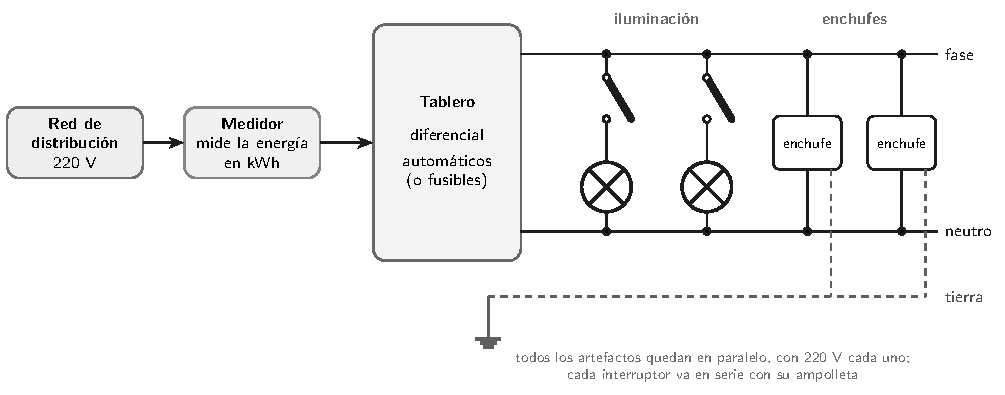
\includegraphics[max width=0.92\linewidth,max height=8.5cm]{fis/ele_instalacion}
\end{center}
  
\begin{itemize}
  \item \textbf{Medidor:} registra la energía consumida, en kWh. Con sus lecturas se calcula la cuenta.
  \item \textbf{Tablero:} reparte la energía en varios circuitos (iluminación, enchufes, cocina) y contiene las protecciones, como el diferencial.
\end{itemize}
  
\begin{itemize}
  \item \textbf{Diferencial:} detecta fugas de corriente a tierra (por ejemplo, a través de una persona que toca un artefacto dañado) y corta en milésimas de segundo. Protege a las personas.
  \item \textbf{Conexión a tierra:} el terminal central del enchufe une la carcasa metálica de los artefactos con la tierra, para que una fuga se descargue por ese cable y no a través de quien toca el artefacto.
  \item \textbf{Enchufes y ampolletas:} conectados \textbf{en paralelo}, todos reciben 220 V y funcionan de forma independiente. Cada interruptor va \textbf{en serie} con la ampolleta que controla.
\end{itemize}
 
\begin{clave}[{Recuerda}] Los aparatos que funcionan con un voltaje menor (celulares, notebooks) usan un cargador con un \textbf{transformador}, que reduce los 220 V de la red al voltaje que necesitan.\end{clave}
\subsection{Lo clave del tema}
\begin{center}\small
\begin{tabularx}{\linewidth}{@{}>{\raggedright\arraybackslash\hsize=0.74\hsize}X>{\raggedright\arraybackslash\hsize=1.64\hsize}X>{\raggedright\arraybackslash\hsize=0.62\hsize}X@{}}
\toprule
\textbf{Concepto} & \textbf{Fórmula o función} & \textbf{Unidad} \\
\midrule
Potencia eléctrica & $P = V\cdot I = I^2 R = V^2/R$ & watt (W) \\
Energía & $E = P\cdot t$ & joule (J) o kWh \\
Kilowatt hora & 1 kWh = 3.600.000 J & kWh \\
Costo & energía en kWh × precio del kWh & pesos \\
Medidor & registra la energía consumida & kWh \\
Diferencial & corta si detecta una fuga de corriente a tierra &  \\
Conexión a tierra & desvía las fugas de la carcasa a tierra &  \\
\bottomrule
\end{tabularx}
\end{center}
 
\begin{clave}[{Recuerda}] · En una casa todo está en paralelo a 220 V: más artefactos encendidos, más corriente total.\par · La potencia dice qué tan rápido se consume la energía; el costo depende también del tiempo.\par · El medidor registra la energía consumida, no la potencia.\end{clave}
 
\begin{clave}[{Método PAES}] 1. Identifica qué piden: potencia, energía, costo, corriente o un componente. 2. Pasa las unidades: W a kW y minutos a horas para kWh; segundos para joule. 3. Elige la forma de la potencia que use tus datos ($VI$, $I^2R$ o $V^2/R$). 4. En instalaciones, recuerda que todo está en paralelo a 220 V: cada artefacto suma su corriente a la total.\end{clave}
\begin{elejemplo}{Estilo PAES}
En una casa se usa un hervidor de 2000 W durante 15 minutos al día, todos los días de un mes de 30 días. El precio de la energía eléctrica es de 180 pesos por kWh.

¿Cuánto cuesta la energía que consume el hervidor en ese mes?
\alts{90 pesos}{2.700 pesos}{162.000 pesos}{2.700.000 pesos}
\solucion{\textbf{Paso 1. ¿Qué nos piden?} El costo mensual del consumo de un artefacto.

\textbf{Paso 2. Pasa a las unidades del kWh.} Potencia: 2000 W = 2 kW. Tiempo diario: 15 min = 0,25 h. Tiempo en el mes: $0{,}25\cdot 30 = 7{,}5$ h.

\textbf{Paso 3. Calcula la energía.} $E = P\cdot t = 2\cdot 7{,}5 = 15$ kWh.

\textbf{Paso 4. Calcula el costo.} $15\cdot 180 = 2700$ pesos.

\textbf{Respuesta:} 2.700 pesos.

\textbf{¿Por qué no las otras?} 90 pesos es el costo de un solo día (0,5 kWh): falta multiplicar por los 30 días. 162.000 pesos sale de usar 15 horas en vez de 15 minutos. 2.700.000 pesos sale de dejar la potencia en W en lugar de pasarla a kW.

\textbf{\color{cienciaD}Para recordar.} Costo = potencia en kW × horas de uso × precio del kWh.}{B}
\end{elejemplo}

\chapter{Habilidades científicas}
%% =====================================================================
%% fis_hab_investigacion
\section[Preguntas, hipótesis y variables]{Preguntas, hipótesis y variables}
\modcomun\ \ {\color{gris}\itshape Cómo se arma una investigación en física: pregunta investigable, hipótesis y predicción, variables independiente, dependiente y controladas, ensayo de referencia, instrumentos de medición, componentes de una investigación y un diseño experimental que cambie solo una variable.\par}
\subsection{La investigación científica paso a paso}
Buena parte de la PAES de Física no te pide una fórmula: te describe un experimento con péndulos, resortes, láseres o circuitos y te pregunta por su \textbf{pregunta}, su \textbf{hipótesis}, sus \textbf{variables} o su \textbf{conclusión}. Todas esas preguntas siguen el mismo esquema.

  

\textbf{Un ejemplo completo.}

 

\textbf{1. Observación.} Un columpio con cadenas largas va y viene más lento que uno con cadenas cortas.

 

\textbf{2. Pregunta.} ¿Cómo influye el largo de un péndulo en su período?

 

\textbf{3. Hipótesis.} El largo del péndulo influye en su período.

 

\textbf{4. Predicción.} Si la hipótesis es correcta, un péndulo de 100 cm tardará más en completar una oscilación que uno de 25 cm.

 

\textbf{5. Procedimiento.} Se cuelga la misma masa de hilos de 25, 50, 75 y 100 cm, se suelta siempre desde 10° y se mide con un cronómetro el tiempo de 10 oscilaciones, que luego se divide por 10.

 

\textbf{6. Resultados.} 1,0 s; 1,4 s; 1,7 s y 2,0 s.

 

\textbf{7. Conclusión.} En el rango estudiado, a mayor largo del péndulo, mayor es su período.

  
\begin{clave}[{Pregunta investigable}] Es una pregunta que se puede responder \textbf{midiendo} u observando algo. Casi siempre relaciona dos variables: «¿cómo influye A en B?».\end{clave}
 
\begin{clave}[{¿Investigable o no?}] · «¿Influye la tensión de una cuerda en la rapidez de las ondas que viajan por ella?»: sí, se cambia la tensión y se mide la rapidez.\par · «¿Es la luz azul más bonita que la roja?»: no, es una opinión.\par · «¿Qué día exacto ocurrirá el próximo gran sismo en Valparaíso?»: no se puede responder con mediciones hoy.\end{clave}
 
\begin{clave}[{Recuerda}] La pregunta de investigación calza con el procedimiento. Si un estudiante cierra un circuito y anota la corriente cada cinco minutos, la pregunta es «¿cómo cambia la intensidad de corriente con el tiempo de funcionamiento?», no una pregunta sobre el voltaje o el interruptor.\end{clave}
\subsection{Hipótesis y predicción}
La \textbf{hipótesis} es una respuesta tentativa a la pregunta. Tiene tres rasgos:

 
\begin{itemize}
  \item Se plantea \textbf{antes} del experimento.
  \item Relaciona la variable que se cambia con la que se mide: «la temperatura del agua influye en la refracción de la luz».
  \item Se puede poner a prueba, y podría resultar falsa.
\end{itemize}
 

La \textbf{predicción} es más concreta: dice qué resultado se espera en \textbf{este} experimento si la hipótesis es cierta. Suele tener la forma «si\dots{}, entonces\dots{}».

 
\begin{center}\small
\begin{tabularx}{\linewidth}{@{}>{\raggedright\arraybackslash\hsize=1.00\hsize}X>{\raggedright\arraybackslash\hsize=1.00\hsize}X@{}}
\toprule
\textbf{Hipótesis} & \textbf{Predicción} \\
\midrule
La tensión de una cuerda influye en la rapidez de las ondas que viajan por ella. & Si se cuelga el doble de masa del extremo de la cuerda, el pulso recorrerá los 2 m en menos tiempo. \\
La temperatura del agua influye en la refracción de la luz. & Al calentar el agua, el ángulo de refracción del láser cambiará. \\
El largo de un conductor influye en su resistencia eléctrica. & Una barra de grafito de 20 cm tendrá más resistencia que una de 10 cm del mismo grosor. \\
\bottomrule
\end{tabularx}
\end{center}
  
\begin{ejemplo}[{Ejemplo resuelto: ¿qué hipótesis se puso a prueba?}] Un cilindro con agua y un émbolo tiene tres orificios a distintas profundidades, cada uno conectado a un tubo en U. Los estudiantes anotan la altura del líquido en cada tubo, presionan el émbolo y vuelven a anotar: las tres alturas suben.\par \textbf{Paso 1.} ¿Qué cambia? La presión sobre la superficie del líquido (se presiona el émbolo).\par \textbf{Paso 2.} ¿Qué se mide? La altura en cada tubo, que indica la presión en cada punto del líquido.\par \textbf{Paso 3.} La hipótesis une ambas: «al aumentar la presión sobre la superficie de un líquido, aumenta la presión en todos sus puntos».\par Una hipótesis sobre la densidad del líquido o el área de los orificios no se pone a prueba aquí: esas variables no cambiaron.\end{ejemplo}
 
\begin{clave}[{Recuerda}] La hipótesis va antes de experimentar; la conclusión, después, apoyada en los datos. Un experimento no «demuestra» una hipótesis para siempre: la apoya o la contradice.\end{clave}
\subsection{Variables: independiente, dependiente y controladas}
\begin{center}
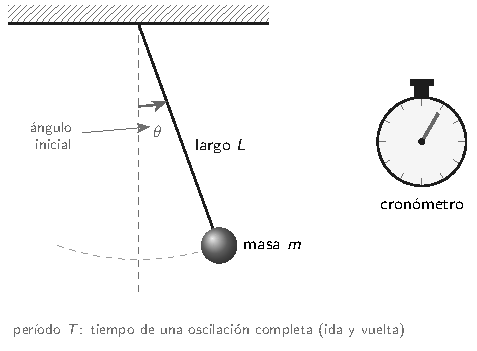
\includegraphics[max width=0.92\linewidth,max height=8.5cm]{fis/hab_pendulo}
\end{center}
  

En el péndulo del ejemplo se cambia el largo del hilo y se mide el período con un cronómetro.

 
\begin{center}\small
\begin{tabularx}{\linewidth}{@{}>{\raggedright\arraybackslash\hsize=0.50\hsize}X>{\raggedright\arraybackslash\hsize=1.25\hsize}X>{\raggedright\arraybackslash\hsize=1.25\hsize}X@{}}
\toprule
\textbf{Variable} & \textbf{Cómo reconocerla} & \textbf{En el péndulo} \\
\midrule
\textbf{Independiente} & La que el investigador \textbf{cambia a propósito} (la causa). & Largo del hilo \\
\textbf{Dependiente} & La que se \textbf{mide} como respuesta (el efecto). & Período de oscilación \\
\textbf{Controladas} & Las que se dejan \textbf{iguales} para que no influyan. & Masa, ángulo inicial, tipo de hilo, forma de medir el tiempo \\
\bottomrule
\end{tabularx}
\end{center}
 
\gatotip[\gatoatigrado]{\textbf{Truco de la frase.} Arma la frase «el efecto de \textbf{[independiente]} sobre \textbf{[dependiente]}». Aquí: «el efecto del largo sobre el período». Si la frase no tiene sentido, cambiaste el orden.}
  
\begin{ejemplo}[{Ejemplo resuelto}] Con una fuente de poder variable, un estudiante aplica 2, 4, 6 y 8 V a un mismo resistor y mide la corriente con un amperímetro. Todo a temperatura ambiente.\par · Cambia a propósito: la diferencia de potencial \ensuremath{\rightarrow} \textbf{independiente}.\par · Se mide al final: la intensidad de corriente \ensuremath{\rightarrow} \textbf{dependiente}.\par · Siempre igual: el resistor y la temperatura \ensuremath{\rightarrow} \textbf{controladas}.\end{ejemplo}
 
\begin{clave}[{Recuerda}] Si cambias la masa de un bloque, también cambian su peso y la fuerza normal que el piso ejerce sobre él: esas fuerzas no son variables controladas. Una variable controlada es algo que de verdad se mantiene igual en todos los ensayos, como la superficie, la compresión del resorte o el ángulo de lanzamiento.\end{clave}
\subsection{Ensayo de referencia, comparaciones justas e instrumentos}
El \textbf{grupo control} o \textbf{ensayo de referencia} es la medición sin el factor que se estudia. Para saber cuánto bloquea una caja metálica la señal de un celular, se mide la señal fuera de la caja (referencia) y dentro de ella. Sin la referencia no sabrías si la caja hizo algo.

 

\textbf{Compara solo ensayos que se diferencian en una cosa.}

 
\begin{center}\small
\begin{tabular}{@{}lll@{}}
\toprule
\textbf{Ensayo} & \textbf{Largo (cm)} & \textbf{Masa (g)} \\
\midrule
1 & 50 & 100 \\
2 & 100 & 100 \\
3 & 100 & 200 \\
\bottomrule
\end{tabular}
\end{center}
 

· 1 y 2: solo cambia el largo \ensuremath{\rightarrow} sirven para estudiar el largo.\par · 2 y 3: solo cambia la masa \ensuremath{\rightarrow} sirven para estudiar la masa.\par · 1 y 3: cambian dos cosas \ensuremath{\rightarrow} no permiten saber cuál causó la diferencia.

 
\begin{center}
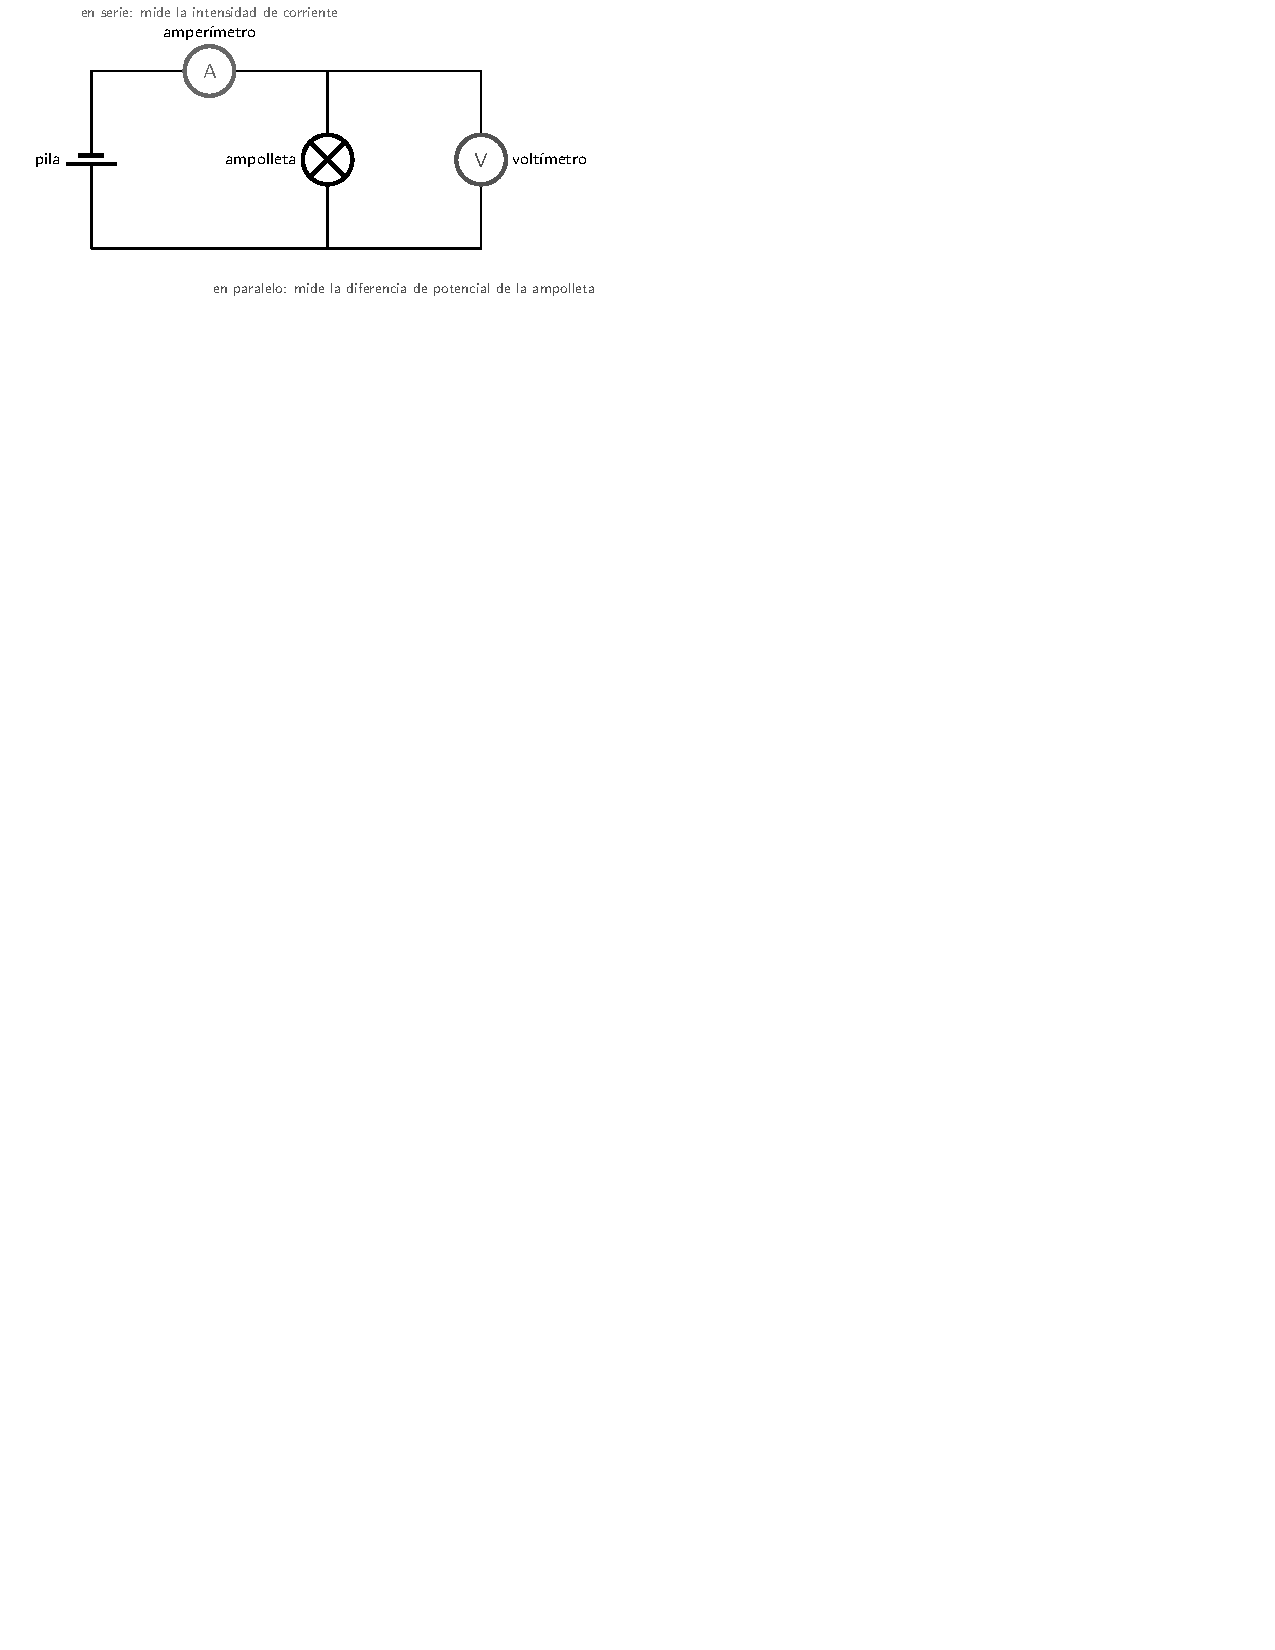
\includegraphics[max width=0.92\linewidth,max height=8.5cm]{fis/hab_circuito}
\end{center}
  
\begin{clave}[{Instrumentos según la variable}] \begin{center}\small
\begin{tabular}{@{}ll@{}}
\toprule
\textbf{Para medir\dots{}} & \textbf{se usa\dots{}} \\
\midrule
longitud, deformación de un resorte & regla o huincha \\
masa & balanza \\
fuerza (peso, tensión, roce) & dinamómetro \\
tiempo, período & cronómetro \\
ángulos (reflexión, refracción) & transportador \\
posición y rapidez de un móvil & sensor de movimiento \\
temperatura & termómetro \\
intensidad de corriente & amperímetro, en serie \\
diferencia de potencial & voltímetro, en paralelo \\
resistencia eléctrica & óhmetro (multímetro) \\
energía eléctrica consumida & medidor eléctrico (kWh) \\
vibraciones del suelo & sismógrafo \\
\bottomrule
\end{tabular}
\end{center}\end{clave}
 
\begin{clave}[{Recuerda}] Antes de elegir un instrumento, identifica qué variable piden. Si se estudia cómo la masa de un objeto influye en la fuerza necesaria para moverlo, la balanza mide la variable independiente y el dinamómetro, la dependiente.\end{clave}
\subsection{Los componentes de una investigación}
La PAES pregunta mucho «¿a qué componente de la investigación corresponde la frase entre comillas?». Apréndete esta tabla:

 
\begin{center}\small
\begin{tabularx}{\linewidth}{@{}>{\raggedright\arraybackslash\hsize=0.62\hsize}X>{\raggedright\arraybackslash\hsize=1.19\hsize}X>{\raggedright\arraybackslash\hsize=1.19\hsize}X@{}}
\toprule
\textbf{Componente} & \textbf{Qué es} & \textbf{Ejemplo en física} \\
\midrule
\textbf{Marco conceptual} & Lo que ya se sabe: leyes, teorías y modelos. & «Según la ley de Hooke, la deformación de un resorte es proporcional a la fuerza». \\
\textbf{Problema / pregunta} & Lo que se quiere averiguar. & «¿Cómo influye el ángulo de tiro en la aceleración de una maleta?». \\
\textbf{Objetivo} & Lo que se quiere lograr; empieza con un verbo en infinitivo. & «Determinar la relación entre el largo de una barra de grafito y su resistencia». \\
\textbf{Hipótesis} & Respuesta tentativa que se pone a prueba. & «La tensión de la cuerda influye en la rapidez de la onda». \\
\textbf{Predicción} & Resultado concreto esperado. & «Si suelto las dos esferas a la vez, llegarán juntas al suelo». \\
\textbf{Procedimiento} & Los pasos que se siguen. & «Se colgaron masas de 100 g y se midió el estiramiento con una regla». \\
\textbf{Observación} & Lo que se percibe directamente. & «Los paracaidistas no llegaron al suelo al mismo tiempo». \\
\textbf{Resultado / evidencia} & Los datos obtenidos. & «El ángulo de refracción del haz violeta fue 40,19°». \\
\textbf{Inferencia} & Interpretación que va más allá de lo observado. & «Los paracaídas deben tener tamaños distintos». \\
\textbf{Conclusión} & Respuesta a la pregunta, apoyada en los resultados. & «La fuerza de roce no depende del área de contacto». \\
\bottomrule
\end{tabularx}
\end{center}
  
\begin{clave}[{Pistas en el texto}] · «si\dots{}, entonces\dots{} ocurrirá»: predicción.\par · «determinar», «comparar», «evaluar», en infinitivo: objetivo.\par · «se colgó, se midió, se repitió»: procedimiento.\par · «se obtuvo», «los valores fueron»: resultado.\par · «debe ser», «esto sugiere», «podría indicar»: inferencia.\par · Responde la pregunta a partir de los datos: conclusión.\end{clave}
  
\begin{clave}[{Recuerda}] Observar es registrar lo que se ve («no todos llegan juntos»). Inferir es proponer algo que no se vio, a partir de lo observado y de lo que se sabe («entonces los paracaídas deben ser de distinto tamaño»). La conclusión, en cambio, sale de los resultados de una investigación diseñada para responder una pregunta.\end{clave}
\subsection{Diseñar un procedimiento y reconocer su objetivo}
Un buen procedimiento sigue cinco pasos:

 

\textbf{Paso 1.} Lee el objetivo y nombra la variable independiente (la que vas a cambiar) y la dependiente (la que vas a medir).

 

\textbf{Paso 2.} Elige varios valores de la independiente: 25, 50, 75 y 100 cm.

 

\textbf{Paso 3.} Deja \textbf{todo lo demás igual}: misma masa, mismo ángulo inicial, mismo hilo.

 

\textbf{Paso 4.} Decide con qué instrumento medirás la dependiente: cronómetro.

 

\textbf{Paso 5.} \textbf{Repite} cada medición y saca un promedio.

 
\begin{clave}[{Recuerda}] El objetivo de una investigación calza con lo que se varió y con lo que se midió. Si una persona tira de una maleta con la misma fuerza, cambia el ángulo y mide la aceleración, su objetivo es «determinar el efecto del ángulo sobre la aceleración», no sobre el peso ni sobre la magnitud de la fuerza.\end{clave}
  
\begin{ejemplo}[{Ejemplo resuelto: un modelo para estudiar un fenómeno}] Se quiere estudiar cómo el área de la sección transversal de un conductor afecta su capacidad de conducir corriente. Como la corriente se parece a un flujo de agua, se usan dos contenedores a distinta altura unidos por un tubo.\par \textbf{Paso 1.} ¿Qué representa cada parte? El tubo es el conductor; su \textbf{radio} representa el área de la sección; el caudal de agua representa la corriente.\par \textbf{Paso 2.} ¿Qué se varía? El radio del tubo.\par \textbf{Paso 3.} ¿Qué se mide? Qué tan rápido se llena el contenedor de abajo (el caudal).\par \textbf{Paso 4.} ¿Qué se deja igual? El largo del tubo, la diferencia de altura y el volumen inicial de agua.\par Variar el largo del tubo o la diferencia de altura estudiaría otras variables (el largo del conductor o el voltaje).\end{ejemplo}
\subsection{Lo clave del tema}
\begin{center}\small
\begin{tabularx}{\linewidth}{@{}>{\raggedright\arraybackslash\hsize=0.96\hsize}X>{\raggedright\arraybackslash\hsize=1.04\hsize}X@{}}
\toprule
\textbf{Concepto} & \textbf{Lo que tienes que reconocer} \\
\midrule
Pregunta de investigación & Se responde midiendo; calza con lo que se varió y lo que se midió. \\
Hipótesis & Respuesta tentativa que relaciona la variable independiente con la dependiente. \\
Predicción & Resultado concreto esperado: «si\dots{}, entonces\dots{}». \\
Variable independiente & La que se cambia a propósito. \\
Variable dependiente & La que se mide. \\
Variables controladas & Las que se mantienen iguales en todos los ensayos. \\
Ensayo de referencia & Medición sin el factor estudiado, para comparar. \\
Instrumento & El que mide la variable pedida: regla, balanza, dinamómetro, cronómetro, amperímetro, voltímetro\dots{} \\
Observación / inferencia / conclusión & Lo que se ve / lo que se deduce más allá / la respuesta a la pregunta con los datos. \\
\bottomrule
\end{tabularx}
\end{center}
 
\begin{clave}[{Recuerda}] · Para estudiar una variable, compara ensayos que solo difieren en esa variable.\par · Si cambias la masa, también cambian el peso y la normal: no son controladas.\par · La hipótesis habla de la variable que cambia en el experimento.\par · El amperímetro va en serie y el voltímetro en paralelo.\par · El instrumento que registra el resultado suele delatar la variable dependiente.\end{clave}
 
\begin{clave}[{Método PAES}] 1. Subraya qué se cambió, qué se midió y qué se dejó igual. 2. Con eso, nombra las tres variables. 3. Si preguntan por la hipótesis, la pregunta o el objetivo, elige la que relaciona exactamente esas dos variables. 4. Si preguntan por un componente, busca las pistas («si\dots{} entonces», «se obtuvo», «debe ser»). 5. Descarta las alternativas que hablan de variables que no cambiaron.\end{clave}
\begin{elejemplo}{Estilo PAES}
Un grupo de estudiantes investiga de qué depende el período de un péndulo. Arma cuatro péndulos como el de la figura y los suelta en las condiciones de la tabla:

\begin{center}\small
\begin{tabular}{@{}llll@{}}
\toprule
\textbf{Ensayo} & \textbf{Largo del hilo (cm)} & \textbf{Masa (g)} & \textbf{Ángulo inicial (°)} \\
\midrule
1 & 50 & 100 & 10 \\
2 & 100 & 100 & 10 \\
3 & 100 & 200 & 10 \\
4 & 50 & 200 & 20 \\
\bottomrule
\end{tabular}
\end{center}

¿Qué par de ensayos permite estudiar el efecto de la \textbf{masa} sobre el período?
\begin{center}
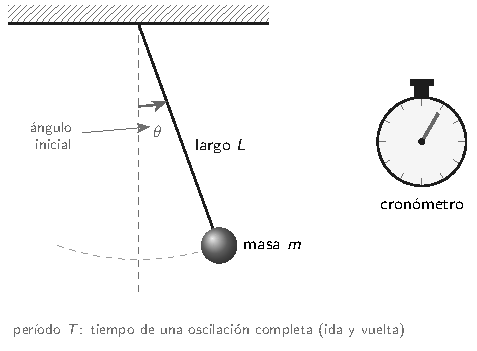
\includegraphics[max width=0.92\linewidth,max height=8.5cm]{fis/hab_pendulo}
\end{center}
\alts{Los ensayos 1 y 2.}{Los ensayos 2 y 3.}{Los ensayos 1 y 4.}{Los ensayos 3 y 4.}
\solucion{\textbf{Paso 1. ¿Qué nos piden?} Un par de ensayos que sirva para estudiar la masa. Dos ensayos sirven para estudiar una variable solo si se diferencian \textbf{únicamente} en esa variable; así, si el período cambia, sabemos qué lo causó.

\textbf{Paso 2. Ensayos 1 y 2.} Largo: 50 y 100 (cambia). Masa: 100 y 100 (igual). Ángulo: 10 y 10 (igual). Solo cambia el largo: este par sirve para estudiar el \textbf{largo}, no la masa.

\textbf{Paso 3. Ensayos 2 y 3.} Largo: 100 y 100 (igual). Masa: 100 y 200 (cambia). Ángulo: 10 y 10 (igual). Solo cambia la masa: este par sirve. \ding{52}

\textbf{Paso 4. Ensayos 1 y 4.} Largo igual, pero cambian la masa (100 y 200) y el ángulo (10 y 20). Con dos cambios a la vez no se puede atribuir la diferencia a la masa.

\textbf{Paso 5. Ensayos 3 y 4.} Masa igual (200), pero cambian el largo y el ángulo. No sirve.

\textbf{Respuesta:} los ensayos 2 y 3.

\textbf{Comprobación:} en los ensayos 2 y 3 la masa es la variable independiente; el largo (100 cm) y el ángulo (10°) son variables controladas. Si los estudiantes hacen el experimento, encontrarán que el período casi no cambia: para ángulos pequeños, el período de un péndulo no depende de la masa.

\textbf{¿Por qué no las otras?} En los ensayos 1 y 2 la masa es la misma: ese par estudia el largo. En los pares 1 y 4 y 3 y 4 cambian dos variables a la vez, así que cualquier diferencia en el período podría deberse a cualquiera de ellas.

\textbf{\color{cienciaD}Para recordar.} Para estudiar una variable, compara solo ensayos que se diferencian únicamente en esa variable.}{B}
\end{elejemplo}

%% =====================================================================
%% fis_hab_evidencia
\section[Procesar y analizar evidencia]{Procesar y analizar evidencia}
\modcomun\ \ {\color{gris}\itshape Leer tablas y gráficos de experimentos de física, reconocer tendencias y relaciones de proporcionalidad directa e inversa, interpretar la pendiente, interpolar y predecir con cuidado, hacer cálculos rápidos con los datos y elegir conclusiones que se apoyan en ellos.\par}
\subsection{Leer una tabla de datos}
Antes de mirar las alternativas, lee la tabla en este orden:

 

\textbf{1. Encabezados y unidades.} ¿Qué variable está en cada columna y en qué unidad?

 

\textbf{2. ¿Cuál se cambió?} Suele ser la primera columna, con valores «redondos» (0, 10, 20, 30).

 

\textbf{3. Tendencia.} Recorre la columna medida de arriba abajo: ¿sube, baja, se mantiene, sube y luego baja?

 

\textbf{4. Compara de a pares.} «Cuando la temperatura aumenta, la rapidez aumenta».

 
\begin{center}\small
\begin{tabular}{@{}ll@{}}
\toprule
\textbf{Temperatura del aire (°C)} & \textbf{Rapidez del sonido (m/s)} \\
\midrule
0 & 331 \\
10 & 337 \\
20 & 343 \\
30 & 349 \\
\bottomrule
\end{tabular}
\end{center}
  
\begin{ejemplo}[{Ejemplo resuelto}] En la tabla, ¿cómo se relacionan las variables?\par \textbf{Paso 1.} Tendencia: a mayor temperatura, mayor rapidez del sonido.\par \textbf{Paso 2.} Variación: cada 10 °C la rapidez aumenta 6 m/s. El aumento es constante: la relación es \textbf{lineal}.\par \textbf{Paso 3.} ¿Es proporcional? No: a 0 °C la rapidez no es cero (es 331 m/s), y al duplicar la temperatura de 10 a 20 °C la rapidez no se duplica.\par \textbf{Conclusión:} en el rango estudiado, la rapidez del sonido aumenta en forma lineal con la temperatura.\end{ejemplo}
 
\begin{clave}[{Recuerda}] Cuando una tabla tiene varias columnas medidas (altitud, presión, temperatura, densidad), cada afirmación de las alternativas relaciona solo dos. Revísalas de a una, leyendo bien el sentido: «disminuye cuando la altitud disminuye» es lo opuesto de «disminuye cuando la altitud aumenta».\end{clave}
\subsection{Leer un gráfico}
\begin{center}
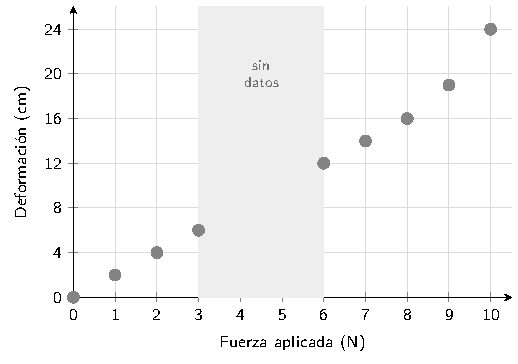
\includegraphics[max width=0.92\linewidth,max height=8.5cm]{fis/hab_hooke}
\end{center}
  

\textbf{1. Ejes.} ¿Qué variable va en cada eje y con qué unidad? Aquí: fuerza aplicada (N) en el eje horizontal, deformación del resorte (cm) en el vertical.

 

\textbf{2. Forma.} Entre 0 y 8 N los puntos están sobre una recta que pasa por el origen: la deformación es \textbf{proporcional} a la fuerza (ley de Hooke), 2 cm por cada newton.

 

\textbf{3. Zonas.} Con 9 y 10 N la deformación crece más rápido: el resorte \textbf{deja de cumplir la ley de Hooke}; se acerca o supera su límite elástico.

 

\textbf{4. Huecos.} Entre 3 y 6 N no hay mediciones. Se puede estimar con la tendencia de los puntos vecinos.

 
\begin{clave}[{Recuerda}] Un punto aislado no es una tendencia. Mira el conjunto de puntos y fíjate dónde cambia el comportamiento: ahí suele estar la respuesta.\end{clave}
\subsection{Relaciones entre variables}
\begin{center}
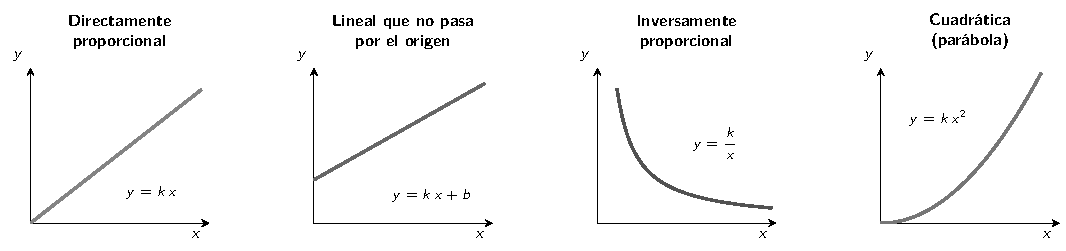
\includegraphics[max width=0.92\linewidth,max height=8.5cm]{fis/hab_relaciones}
\end{center}
  
\begin{center}\small
\begin{tabularx}{\linewidth}{@{}>{\raggedright\arraybackslash\hsize=0.71\hsize}X>{\raggedright\arraybackslash\hsize=1.14\hsize}X>{\raggedright\arraybackslash\hsize=1.14\hsize}X@{}}
\toprule
\textbf{Relación} & \textbf{Prueba con los datos} & \textbf{Ejemplo en física} \\
\midrule
\textbf{Directamente proporcional} & El \textbf{cociente} $y/x$ es constante. & Ley de Hooke: $F = k\,x$. Ley de Ohm: $V = I\,R$. \\
\textbf{Lineal, no proporcional} & Aumentos iguales, pero no pasa por el origen. & Largo total de un resorte: largo natural + deformación. \\
\textbf{Inversamente proporcional} & El \textbf{producto} $x\cdot y$ es constante. & Ondas en un mismo medio: $\lambda = \dfrac{v}{f}$. \\
\textbf{Cuadrática} & Al duplicar $x$, $y$ se cuadruplica. & Caída libre desde el reposo: $d = 5\,t^2$ (m, s). \\
\bottomrule
\end{tabularx}
\end{center}
  
\begin{ejemplo}[{Ejemplo resuelto}] Por una misma cuerda viajan ondas de 10, 20 y 40 Hz con longitudes de onda de 2,0; 1,0 y 0,5 m.\par \textbf{Paso 1.} Productos: $10\cdot 2{,}0 = 20$; $20\cdot 1{,}0 = 20$; $40\cdot 0{,}5 = 20$.\par \textbf{Paso 2.} El producto es constante: $\lambda$ y $f$ son \textbf{inversamente proporcionales}, y ese producto es la rapidez de la onda, 20 m/s.\end{ejemplo}
 
\begin{clave}[{Recuerda}] «Cuando una aumenta, la otra aumenta» no basta para decir que son proporcionales. Comprueba el cociente: si al duplicar una la otra no se duplica, la relación es otra. El período de un péndulo, por ejemplo, crece con el largo, pero para duplicar el período hay que \textbf{cuadruplicar} el largo.\end{clave}
\subsection{La pendiente en los gráficos de física}
En un gráfico con forma de recta, la \textbf{pendiente} es $\dfrac{\Delta y}{\Delta x}$, y en física casi siempre significa algo:

 
\begin{center}\small
\begin{tabularx}{\linewidth}{@{}>{\raggedright\arraybackslash\hsize=1.03\hsize}X>{\raggedright\arraybackslash\hsize=0.97\hsize}X@{}}
\toprule
\textbf{Gráfico (vertical vs. horizontal)} & \textbf{La pendiente es\dots{}} \\
\midrule
Fuerza vs. deformación & la constante elástica $k$ \\
Diferencia de potencial vs. corriente & la resistencia $R$ \\
Corriente vs. diferencia de potencial & el inverso de la resistencia, $1/R$ \\
Posición vs. tiempo & la velocidad \\
Velocidad vs. tiempo & la aceleración \\
\bottomrule
\end{tabularx}
\end{center}
 
\begin{clave}[{Recuerda}] Fíjate qué variable está en cada eje. Si el gráfico es de corriente en función del voltaje, la recta más empinada corresponde a la resistencia \textbf{menor}, porque deja pasar más corriente con el mismo voltaje.\end{clave}
  
\begin{center}
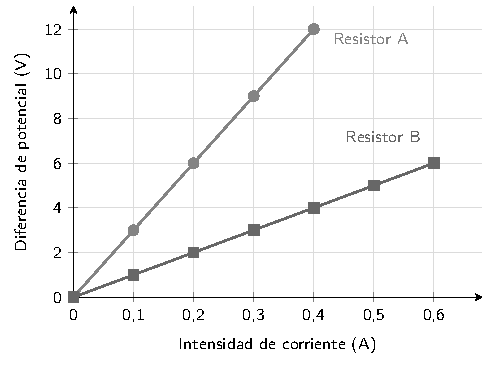
\includegraphics[max width=0.92\linewidth,max height=8.5cm]{fis/hab_ohm}
\end{center}
 
\begin{ejemplo}[{Ejemplo resuelto}] ¿Cuánto vale la resistencia B?\par \textbf{Paso 1.} El gráfico es de voltaje en función de la corriente: la pendiente es $R$.\par \textbf{Paso 2.} Toma un punto de la recta: 6 V con 0,6 A.\par \textbf{Paso 3.} $R = \dfrac{V}{I} = \dfrac{6}{0{,}6} = 10$ \ensuremath{\Omega}.\end{ejemplo}
\subsection{Tendencias: interpolar y predecir}
\textbf{Interpolar} es estimar un valor \textbf{dentro} del rango medido, siguiendo la tendencia. Es confiable si la tendencia es clara.

 

\textbf{Extrapolar} es estimar \textbf{fuera} del rango medido. Es riesgoso: el comportamiento puede cambiar, como el resorte que sobre 8 N deja de cumplir la ley de Hooke.

 
\begin{ejemplo}[{Ejemplo resuelto: interpolar}] Con la tabla de la rapidez del sonido (331 m/s a 0 °C; 337 a 10 °C; 343 a 20 °C; 349 a 30 °C), ¿qué rapidez se espera a 25 °C?\par \textbf{Paso 1.} 25 °C está entre 20 y 30 °C, dentro del rango.\par \textbf{Paso 2.} La rapidez sube 6 m/s cada 10 °C, es decir, 3 m/s cada 5 °C.\par \textbf{Paso 3.} $343 + 3 = 346$ m/s.\end{ejemplo}
  
\begin{ejemplo}[{Ejemplo resuelto: predecir con una relación}] Un péndulo de 1,0 m tiene un período de 2,0 s. ¿Qué largo necesita para un período de 4,0 s?\par \textbf{Paso 1.} El período crece con la raíz del largo: $T = 2\pi\sqrt{L/g}$.\par \textbf{Paso 2.} Para duplicar el período hay que multiplicar el largo por $2^2 = 4$.\par \textbf{Paso 3.} $L = 4{,}0$ m. Pensar «doble de período, doble de largo» daría 2,0 m, un error típico.\end{ejemplo}
 
\begin{clave}[{Recuerda}] Dentro del rango, sigue la tendencia de los puntos vecinos. Fuera del rango, desconfía de cualquier alternativa que afirme un valor exacto o un comportamiento que no se midió.\end{clave}
\subsection{De los datos a la conclusión}
Una conclusión correcta cumple cuatro condiciones:

 

\textbf{1.} Habla de las variables que se \textbf{midieron}.

 

\textbf{2.} Respeta el \textbf{sentido} de la tendencia («a mayor\dots{}, mayor\dots{}»).

 

\textbf{3.} No va más allá del \textbf{rango} estudiado.

 

\textbf{4.} No afirma \textbf{causas} ni mecanismos que los datos no muestran.

 
\begin{center}\small
\begin{tabular}{@{}ll@{}}
\toprule
\textbf{Tensión de la cuerda (N)} & \textbf{Rapidez del pulso (m/s)} \\
\midrule
4 & 10 \\
16 & 20 \\
36 & 30 \\
\bottomrule
\end{tabular}
\end{center}
  
\begin{ejemplo}[{Ejemplo resuelto}] Con la tabla, ¿qué conclusiones se sostienen?\par · «A mayor tensión, mayor rapidez del pulso»: \textbf{sí}, es la tendencia de los datos.\par · «La rapidez es directamente proporcional a la tensión»: \textbf{no}. Al cuadruplicar la tensión (de 4 a 16 N) la rapidez solo se duplica.\par · «Con 100 N la rapidez será de 50 m/s»: es una extrapolación; la tendencia lo sugiere, pero no se midió.\par · «La rapidez no depende del grosor de la cuerda»: \textbf{no} se puede afirmar; el grosor no se varió.\end{ejemplo}
 
\begin{clave}[{Recuerda}] Que una variable no haya cambiado en el experimento no prueba que no influya: solo significa que no se estudió.\end{clave}
\subsection{Lo clave del tema}
\begin{center}\small
\begin{tabularx}{\linewidth}{@{}>{\raggedright\arraybackslash\hsize=0.75\hsize}X>{\raggedright\arraybackslash\hsize=1.25\hsize}X@{}}
\toprule
\textbf{Si te piden\dots{}} & \textbf{Haz esto} \\
\midrule
Leer una tabla & Encabezados y unidades; qué se cambió; tendencia; compara de a pares. \\
Leer un gráfico & Ejes, forma, zonas donde cambia el comportamiento y huecos sin datos. \\
Proporcionalidad directa & Cociente constante; recta que pasa por el origen. \\
Proporcionalidad inversa & Producto constante; curva que baja. \\
Pendiente & Fíjate en los ejes: $k$, $R$, $1/R$, velocidad o aceleración. \\
Predecir & Interpola dentro del rango; desconfía de extrapolar. \\
Conclusión & Solo variables medidas, en el rango estudiado, con el sentido correcto. \\
\bottomrule
\end{tabularx}
\end{center}
 
\begin{clave}[{Recuerda}] · «Aumentan juntas» no es lo mismo que «son proporcionales».\par · Una recta que no pasa por el origen es lineal, pero no proporcional.\par · En $I$ vs. $V$ la pendiente es $1/R$; en $V$ vs. $I$ es $R$.\par · Lo que no se varió no se puede descartar como causa.\par · Fuera del rango medido, el comportamiento puede cambiar.\end{clave}
 
\begin{clave}[{Método PAES}] 1. Identifica las variables y sus unidades. 2. Describe la tendencia con una frase. 3. Si piden una relación, prueba el cociente y el producto. 4. Si piden un valor, ubica si está dentro o fuera del rango. 5. Descarta las alternativas que hablan de variables que no se midieron.\end{clave}
\begin{elejemplo}{PAES Invierno 2027, adaptada}
Un grupo de estudiantes cuelga distintos pesos de un resorte y mide su deformación. Por un problema con el montaje, no pudieron registrar datos entre 3,0 y 6,0 N. Los resultados se muestran en el gráfico.

Según los resultados, ¿qué se espera que ocurra con la deformación del resorte si se aplican fuerzas entre 3,0 y 6,0 N?
\begin{center}
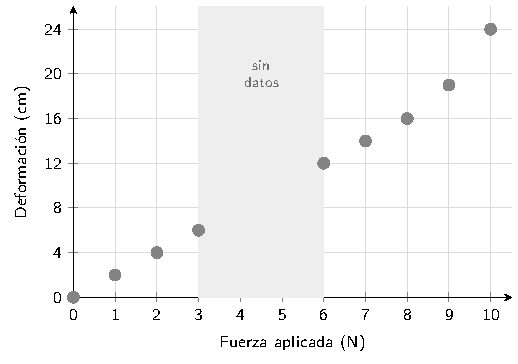
\includegraphics[max width=0.92\linewidth,max height=8.5cm]{fis/hab_hooke}
\end{center}
\altslargas{Se mantendrá en 6 cm, porque en ese tramo no hay datos.}{Disminuirá a medida que la fuerza aumente.}{Tomará valores entre 6 y 12 cm, de unos 2 cm por cada newton; por ejemplo, cerca de 9 cm con 4,5 N.}{Superará los 24 cm, porque el resorte habrá pasado su límite elástico.}
\solucion{\textbf{Paso 1. ¿Qué nos piden?} Estimar la deformación en un tramo sin datos, que está \textbf{dentro} del rango medido: es una interpolación.

\textbf{Paso 2. Mira la tendencia a ambos lados.} Con 1, 2 y 3 N la deformación es 2, 4 y 6 cm. Con 6, 7 y 8 N es 12, 14 y 16 cm. En ambos lados se cumple lo mismo: \textbf{2 cm por cada newton}, una recta que pasa por el origen.

\textbf{Paso 3. Aplica la tendencia al hueco.} Si con 3 N hay 6 cm y con 6 N hay 12 cm, entre medio la deformación irá de 6 a 12 cm. Con 4,5 N: $4{,}5\cdot 2 = 9$ cm.

\textbf{Respuesta:} tomará valores entre 6 y 12 cm, de unos 2 cm por cada newton.

\textbf{¿Por qué no las otras?} Que no haya datos no significa que el resorte deje de estirarse: entre 3 y 6 N la fuerza sigue aumentando. Que disminuya contradice la tendencia, que siempre es creciente. El cambio de comportamiento aparece recién sobre 8 N y con 10 N la deformación es 24 cm: con menos de 6 N no puede superarla.

\textbf{\color{cienciaD}Para recordar.} Para interpolar, sigue la tendencia de los puntos vecinos dentro del rango medido.}{C}
\end{elejemplo}

%% =====================================================================
%% fis_hab_evaluar
\section[Evaluar y comunicar]{Evaluar y comunicar}
\modcomun\ \ {\color{gris}\itshape Distinguir ley, teoría y modelo, reconocer los límites de un modelo (cuerda ideal, resistor óhmico, rayo de luz), evaluar la confiabilidad de las mediciones (repeticiones, precisión, error), juzgar si una conclusión es válida, replicar procedimientos, reconocer aplicaciones tecnológicas y elegir el recurso para comunicar resultados.\par}
\subsection{Ley, teoría y modelo}
\begin{center}\small
\begin{tabularx}{\linewidth}{@{}>{\raggedright\arraybackslash\hsize=0.42\hsize}X>{\raggedright\arraybackslash\hsize=1.29\hsize}X>{\raggedright\arraybackslash\hsize=1.29\hsize}X@{}}
\toprule
\textbf{Componente} & \textbf{Qué es} & \textbf{Ejemplos en física} \\
\midrule
\textbf{Ley} & Describe \textbf{qué pasa}: una regularidad que se cumple siempre en ciertas condiciones. Muchas veces es una relación matemática. & Ley de Hooke, $F = k\,x$. Ley de Ohm, $V = I\,R$. Ley de reflexión: el ángulo de incidencia es igual al de reflexión. Leyes de Newton. \\
\textbf{Teoría} & Explica \textbf{por qué pasa}: una explicación amplia, respaldada por muchas evidencias distintas. & Teoría de la tectónica de placas (explica sismos, volcanes y cordilleras). Teoría electromagnética de la luz. \\
\textbf{Modelo} & Una \textbf{representación simplificada} que sirve para explicar o predecir. & El rayo de luz. La cuerda ideal. El cuerpo como partícula. El modelo dinámico de las capas de la Tierra. La analogía del agua para la corriente. \\
\bottomrule
\end{tabularx}
\end{center}
  
\begin{clave}[{Cómo distinguirlas}] · «La deformación es proporcional a la fuerza»: dice qué pasa \ensuremath{\rightarrow} \textbf{ley}.\par · «Los continentes se mueven porque la litosfera está dividida en placas que se desplazan sobre la astenósfera»: explica por qué \ensuremath{\rightarrow} \textbf{teoría}.\par · «Consideremos la cuerda inextensible y sin masa»: simplifica para calcular \ensuremath{\rightarrow} \textbf{modelo}.\end{clave}
  
\begin{clave}[{Recuerda}] Una teoría no es «una suposición» ni se convierte en ley al acumular pruebas: la ley dice qué pasa y la teoría explica por qué. Son componentes distintos y ninguno pasa a ser el otro. Una teoría bien establecida, como la tectónica de placas, está respaldada por muchísima evidencia.\end{clave}
\subsection{Los modelos tienen límites}
Todo modelo deja algo afuera. Es útil mientras lo que deja afuera no importe; cuando importa, hay que cambiar de modelo.

 
\begin{center}\small
\begin{tabularx}{\linewidth}{@{}>{\raggedright\arraybackslash\hsize=0.62\hsize}X>{\raggedright\arraybackslash\hsize=1.19\hsize}X>{\raggedright\arraybackslash\hsize=1.19\hsize}X@{}}
\toprule
\textbf{Modelo} & \textbf{Supone} & \textbf{Deja de servir cuando\dots{}} \\
\midrule
Cuerda ideal & sin masa e inextensible: la misma tensión en toda la cuerda & la cuerda es gruesa y pesada: la tensión es mayor arriba que abajo \\
Resorte ideal (Hooke) & deformación proporcional a la fuerza & se supera el límite elástico \\
Resistor óhmico & resistencia constante & el conductor se calienta mucho, como el filamento de una ampolleta \\
Rayo de luz & la luz viaja en línea recta & la abertura es comparable a la longitud de onda: aparece la difracción \\
Sin roce & no hay fuerzas que se opongan al movimiento & las superficies son rugosas o el aire frena al objeto \\
\bottomrule
\end{tabularx}
\end{center}
  
\begin{center}
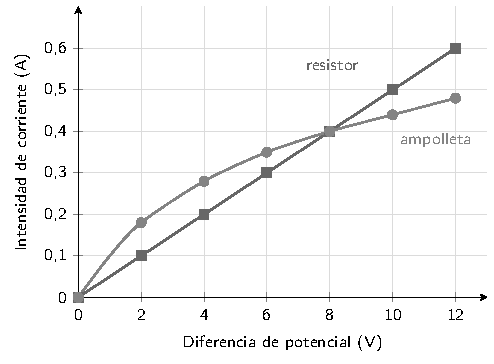
\includegraphics[max width=0.92\linewidth,max height=8.5cm]{fis/hab_no_ohmico}
\end{center}
 
\begin{ejemplo}[{Ejemplo resuelto}] ¿Cumple la ampolleta la ley de Ohm?\par \textbf{Paso 1.} Calcula $R = V/I$ en dos puntos: con 2 V, $\dfrac{2}{0{,}18}\approx 11$ \ensuremath{\Omega}; con 12 V, $\dfrac{12}{0{,}48} = 25$ \ensuremath{\Omega}.\par \textbf{Paso 2.} La resistencia cambia: aumenta porque el filamento se calienta.\par \textbf{Conclusión:} la ampolleta no es un resistor óhmico; la ley de Ohm, con $R$ constante, no la describe bien.\end{ejemplo}
\subsection{Validez, confiabilidad y error de medición}
\begin{center}
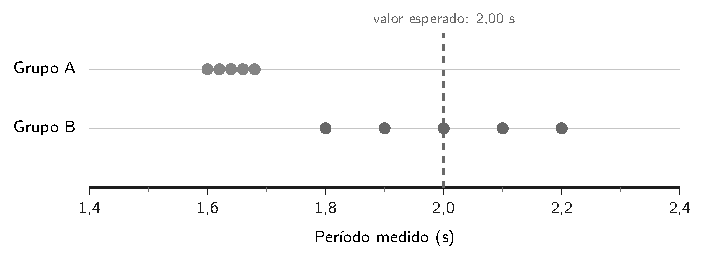
\includegraphics[max width=0.92\linewidth,max height=8.5cm]{fis/hab_mediciones}
\end{center}
  

\textbf{Validez:} la investigación mide de verdad lo que dice medir y su diseño permite responder la pregunta. Falla si cambian dos variables a la vez o si se mide otra variable.

 

\textbf{Confiabilidad:} al repetir la medición se obtienen resultados parecidos. Mejora con más repeticiones y con instrumentos más precisos.

 

\textbf{Precisión y exactitud.} Mediciones \textbf{precisas} están cerca unas de otras. Mediciones \textbf{exactas} están cerca del valor real. En la figura, el grupo A es preciso pero no exacto (quizás su cronómetro o su largo estaban mal); el grupo B tiene un promedio exacto, 2,00 s, pero es menos preciso.

  
\begin{ejemplo}[{Ejemplo resuelto: reducir el error}] Medir con cronómetro una sola oscilación de 2 s tiene un error de reacción de unos 0,2 s, un 10 \%.\par \textbf{Mejora:} medir el tiempo de 10 oscilaciones (unos 20 s) y dividir por 10. El error de reacción sigue siendo de unos 0,2 s, pero repartido en 10 oscilaciones: 0,02 s por oscilación, un 1 \%. Además, conviene repetir la medición y promediar.\end{ejemplo}
 
\begin{clave}[{Recuerda}] Repetir una medición con el mismo error de calibración no la hace exacta: la hace más confiable. Para corregir un error sistemático hay que revisar el instrumento o el montaje.\end{clave}
\subsection{¿La conclusión se sostiene con los datos?}
Para evaluar una conclusión, revisa esta lista:

 

\textbf{1. ¿Responde la pregunta?}

 

\textbf{2. ¿Habla solo de las variables medidas y del rango estudiado?} Si el resorte se probó hasta 5 N, no se puede afirmar qué pasa con 50 N.

 

\textbf{3. ¿Cambió solo una variable?} Si cambiaron dos a la vez, el efecto no se puede atribuir a una.

 

\textbf{4. ¿Hay suficientes repeticiones?}

 

\textbf{5. ¿Se confunde asociación con causa?} Que dos cosas ocurran juntas no prueba que una cause la otra.

  
\begin{ejemplo}[{Ejemplo resuelto}] Una persona pone 1 L de agua recién sacada del refrigerador en el hervidor A y 1 L de agua de la llave en el hervidor B. El agua de B hierve antes y concluye: «el hervidor B es más potente».\par \textbf{Paso 1.} ¿Qué diferencia a los ensayos? El hervidor \textbf{y} la temperatura inicial del agua.\par \textbf{Paso 2.} El agua más fría necesita más energía para llegar a 100 °C, así que puede tardar más aunque el hervidor sea igual de potente.\par \textbf{Evaluación:} la conclusión no se sostiene. Hay que repetir con la misma cantidad de agua a la misma temperatura inicial.\end{ejemplo}
 
\begin{clave}[{Recuerda}] Las alternativas correctas suelen ser prudentes: «en las condiciones del estudio», «en el rango medido», «podría». Desconfía de «siempre», «cualquier» y «demuestra».\end{clave}
\subsection{Replicar, reproducir y mejorar un diseño}
Un procedimiento es \textbf{replicable} si está descrito con tanto detalle que otra persona puede repetirlo. Un resultado es \textbf{reproducible} si al repetirlo se obtiene algo equivalente. Para replicar, hay que mantener las condiciones de las que depende el fenómeno, aunque cambien detalles que no influyen.

 
\begin{center}\small
\begin{tabularx}{\linewidth}{@{}>{\raggedright\arraybackslash\hsize=0.86\hsize}X>{\raggedright\arraybackslash\hsize=1.14\hsize}X@{}}
\toprule
\textbf{Limitación} & \textbf{Mejora} \\
\midrule
Una sola medición & Repetir y promediar. \\
Cambian dos variables a la vez & Cambiar solo la variable independiente. \\
Falta un ensayo de referencia & Medir también sin el factor estudiado. \\
Rango muy estrecho & Ampliar los valores de la variable independiente. \\
Instrumento poco preciso & Usar uno más preciso o medir un intervalo mayor (10 oscilaciones). \\
\bottomrule
\end{tabularx}
\end{center}
  
\begin{ejemplo}[{Ejemplo resuelto}] Un grupo observa el patrón de interferencia de un láser que pasa por dos rendijas muy finas y muy juntas en un papel. Quiere cambiar de láser y seguir viendo un patrón de interferencia. ¿Qué es indispensable mantener?\par \textbf{Paso 1.} ¿De qué depende la interferencia? De que la luz pase por dos aberturas muy pequeñas y cercanas, comparables con la longitud de onda.\par \textbf{Paso 2.} El color o la intensidad del láser cambian el aspecto del patrón (separación de franjas, brillo), pero no impiden que se forme.\par \textbf{Respuesta:} mantener rendijas igual de finas y con una separación similar.\end{ejemplo}
 
\begin{clave}[{Recuerda}] La mejora correcta corrige el defecto que impide responder la pregunta. Si el problema es que cambian dos variables, repetir más veces no lo resuelve.\end{clave}
\subsection{Aplicaciones tecnológicas y comunicar resultados}
\textbf{De la investigación a la tecnología.} La PAES pregunta qué tecnología usa un fenómeno o qué producto podría surgir de un hallazgo.

 
\begin{center}\small
\begin{tabularx}{\linewidth}{@{}>{\raggedright\arraybackslash\hsize=1.00\hsize}X>{\raggedright\arraybackslash\hsize=1.00\hsize}X@{}}
\toprule
\textbf{Fenómeno o hallazgo} & \textbf{Tecnología} \\
\midrule
Reflexión de ondas de radio & radar \\
Materiales piezoeléctricos (voltaje al presionarlos) & chisperos de cocinas y encendedores \\
Radiación infrarroja que emiten los cuerpos tibios & cámaras de visión nocturna \\
Material que bloquea un amplio espectro de radiación & recubrimientos para trajes de astronauta \\
Temperatura de ebullición menor a menor presión atmosférica & sensores de presión en hervidores \\
\bottomrule
\end{tabularx}
\end{center}
  
\begin{center}\small
\begin{tabularx}{\linewidth}{@{}>{\raggedright\arraybackslash\hsize=1.00\hsize}X>{\raggedright\arraybackslash\hsize=1.00\hsize}X@{}}
\toprule
\textbf{Objetivo al comunicar} & \textbf{Recurso} \\
\midrule
Mostrar cómo una variable depende de otra & gráfico de dispersión o de líneas, con la independiente en el eje horizontal \\
Comparar categorías (materiales, colores) & gráfico de barras \\
Entregar valores exactos & tabla \\
Explicar un fenómeno (difracción, refracción) & esquema o modelo del fenómeno \\
Mostrar cómo instalar o conectar algo & plano o diagrama del circuito \\
Informar a la población & afiche con recomendaciones claras \\
\bottomrule
\end{tabularx}
\end{center}
 
\begin{clave}[{Recuerda}] El recurso debe calzar con el objetivo. Si un equipo midió la intensidad de un láser y la profundidad del corte que produce, un gráfico de profundidad en función de la intensidad muestra justo su resultado; un esquema del montaje o una imagen de las ondas no.\end{clave}
\subsection{Lo clave del tema}
\begin{center}\small
\begin{tabularx}{\linewidth}{@{}>{\raggedright\arraybackslash\hsize=0.71\hsize}X>{\raggedright\arraybackslash\hsize=1.29\hsize}X@{}}
\toprule
\textbf{Si te piden\dots{}} & \textbf{Revisa esto} \\
\midrule
Ley, teoría o modelo & Qué pasa / por qué pasa / representación simplificada. \\
Límite de un modelo & Qué supone el modelo y qué dato lo contradice. \\
Confiabilidad & Repeticiones, precisión del instrumento, mediciones cercanas entre sí. \\
Validez & ¿Cambió solo una variable? ¿Se midió la variable del objetivo? \\
Evaluar una conclusión & ¿Sale de los datos? ¿Respeta el rango? ¿Hay variables confundidas? \\
Replicar & Mantener las condiciones de las que depende el fenómeno. \\
Comunicar & El recurso que muestra justo lo que se quiere mostrar. \\
\bottomrule
\end{tabularx}
\end{center}
 
\begin{clave}[{Recuerda}] · Una ley no se transforma en teoría ni al revés.\par · La cuerda ideal, el resorte ideal y el resistor óhmico son modelos con límites.\par · Precisas = cercanas entre sí; exactas = cercanas al valor real.\par · Medir varias oscilaciones y dividir reduce el error del cronómetro.\par · Si dos variables cambian a la vez, la conclusión no se sostiene.\end{clave}
 
\begin{clave}[{Método PAES}] 1. Identifica el objetivo y las variables del estudio. 2. Revisa el diseño: una sola variable cambiada, referencia, repeticiones, instrumento. 3. Compara la alternativa con los datos y con su rango. 4. Desconfía de «siempre», «todos», «cualquier» y «demuestra». 5. Si piden comunicar, elige el recurso según lo que se quiere mostrar.\end{clave}
\begin{elejemplo}{PAES Invierno 2027, adaptada}
Una persona que vive sola registra el consumo eléctrico mensual de su departamento y anota cuándo compra o cambia algún artefacto:

\begin{center}\small
\begin{tabular}{@{}llllllll@{}}
\toprule
\textbf{Mes} & \textbf{May.} & \textbf{Jun.} & \textbf{Jul.} & \textbf{Ago.} & \textbf{Sep.} & \textbf{Oct.} & \textbf{Nov.} \\
\midrule
Consumo (kWh) & 85,3 & 87,6 & 88,4 & 92,1 & 86,2 & 87,4 & 84,2 \\
\bottomrule
\end{tabular}
\end{center}

\textbf{Notas.} Inicio de junio: compré un televisor para ver una serie. Mediados de julio: cambié el refrigerador por uno nuevo que, según el fabricante, consume menos energía. Fines de noviembre: compré un ventilador.

A fin de año, decide reclamarle al fabricante del refrigerador porque no observa que su consumo haya disminuido. ¿Por qué se puede cuestionar su reclamo?
\altslargas{Porque el consumo de agosto es el mayor del registro, lo que prueba que el refrigerador nuevo consume más que el antiguo.}{Porque el registro no informa cuánto se usó cada artefacto cada mes y, en el mismo período, se agregó un televisor, así que no se puede aislar el efecto del refrigerador.}{Porque el ventilador comprado a fines de noviembre explica el aumento del consumo en agosto.}{Porque el consumo eléctrico de un hogar no depende de sus artefactos.}
\solucion{\textbf{Paso 1. ¿Qué nos piden?} Evaluar si los datos permiten concluir que el refrigerador nuevo no redujo el consumo.

\textbf{Paso 2. ¿Qué cambió en el período?} Desde junio hay un televisor nuevo, y a mediados de julio cambió el refrigerador. El consumo total depende de \textbf{todos} los artefactos y de cuánto se usa cada uno.

\textbf{Paso 3. ¿Se puede aislar el refrigerador?} No. El registro solo da el consumo total. Si el televisor se usó mucho (por ejemplo, para ver la serie), su consumo puede tapar el ahorro del refrigerador. Hay dos variables que cambiaron y no hay datos de uso de cada artefacto.

\textbf{Respuesta:} porque el registro no informa cuánto se usó cada artefacto y, en el mismo período, se agregó un televisor.

\textbf{Cómo mejorar:} medir el consumo del refrigerador por separado, o comparar meses con el mismo uso de los demás artefactos.

\textbf{¿Por qué no las otras?} Que agosto sea el mes de mayor consumo total no prueba nada sobre el refrigerador: puede deberse a otros artefactos o a más tiempo en casa. El ventilador se compró a fines de noviembre: no puede explicar agosto. El consumo de un hogar sí depende de sus artefactos; precisamente por eso hay que separar el efecto de cada uno.

\textbf{\color{cienciaD}Para recordar.} Si varias cosas cambian a la vez y solo se mide el total, no se puede atribuir el efecto a una sola.}{B}
\end{elejemplo}
